\documentclass[letterpaper,11pt]{scrreprt}
\usepackage[american]{babel}
\usepackage[latin1]{inputenc}
\usepackage[T1]{fontenc}
\usepackage[top=1in,bottom=1in,left=1in,right=1in]{geometry}
\usepackage{lmodern}

\usepackage[sumlimits]{amsmath}
\usepackage{amssymb}
\usepackage{relsize}
\usepackage[hyperref]{ntheorem}
\usepackage[
	bookmarks,
	colorlinks=false,
	breaklinks=true,
	linkcolor=blue,
	citecolor=blue,
	pagebackref=false,
	pdftitle={MADlib Design Document},
	pdfauthor={Predictive Analytics Team, Pivotal Inc.},
	pdfsubject={},
	pdfkeywords={}
]{hyperref}
\usepackage{csquotes}                  % Strongly recommended for biblatex
\usepackage[
	backend=bibtex,
	maxnames=2,
	maxbibnames=20,
	firstinits=true
]{biblatex}
\usepackage{scrpage2}                  % Headers and footers
\usepackage{scrhack}
\usepackage{color}                     % Colors, possibly only for \todo
\usepackage{enumitem}                  % enumerate environment
\usepackage{ctable}
\usepackage{tabularx}
\usepackage{xspace}                    % Correct spaces after \newcommand definitions
\usepackage[noend]{algpseudocode}      % algorithm environment
\usepackage{listings}                  % Code snippets
\usepackage{bbding}

% BEGIN Doc Layout
	\allowdisplaybreaks[3]

	\pagestyle{scrheadings}
	\automark[chapter]{section}

	\setkomafont{disposition}{\normalcolor\bfseries}
	\setkomafont{descriptionlabel}{\bfseries}
	\setkomafont{captionlabel}{\usekomafont{disposition}}

	\setlength{\arrayrulewidth}{.5pt}
	\numberwithin{equation}{section}
	\renewcommand{\theenumi}{\roman{enumi}}
	\renewcommand{\labelenumi}{\theenumi)}

	\newcommand{\otoprule}{\midrule[\heavyrulewidth]}

	\setcounter{secnumdepth}{3}

	\makeatletter
	% Algorithms are expected to have an optional argument of form
	% FunctionName$(ArgumentList)$, e.g., DiscreteSample$(A, w)$
	\def\internal@funcName#1$(#2)${#1}
	\newcommand\funcName[1]{\internal@funcName #1}
	\newtheoremstyle{algorithm}
		{\item[\rlap{\vbox{\hbox{\hskip\labelsep \theorem@headerfont
			##1\ ##2\theorem@separator}\hbox{\strut}}}]}%
		{\item[\rlap{\vbox{\hbox{\hskip\labelsep {\theorem@headerfont
			##1}\ \normalfont\texttt{##3}{\theorem@headerfont\theorem@separator}}\hbox{\strut}}}]%
			\def\@currentlabel{\texttt{\funcName{##3}}}}
	\makeatother

	\makeatletter
	% Also display JSTOR in small caps
	% http://sourceforge.net/tracker/index.php?func=detail&aid=3152938&group_id=244752&atid=1126006
	\DeclareFieldFormat{eprint:arxiv}{%
	  \textsc{arXiv}\addcolon
	  \ifhyperref
	    {\href{http://arxiv.org/\abx@arxivpath/#1}{%
	       \nolinkurl{#1}%
	       \iffieldundef{eprintclass}
		 {}
		 {\addspace\texttt{\mkbibbrackets{\thefield{eprintclass}}}}}}
	    {\nolinkurl{#1}
	     \iffieldundef{eprintclass}
	       {}
	       {\addspace\texttt{\mkbibbrackets{\thefield{eprintclass}}}}}}
	\DeclareFieldFormat{eprint:jstor}{%
	  \mkbibacro{JSTOR}\addcolon\space
	  \ifhyperref
	    {\href{http://www.jstor.org/stable/#1}{\nolinkurl{#1}}}
	    {\nolinkurl{#1}}}
	% Some conferences do not have DOIs for their papers, but they do get
	% IDs in the ACM Digital Library. E.g., SODA papers.
	\DeclareFieldFormat{eprint:acm}{%
	  \mkbibacro{ACM}\addcolon\space
	  \ifhyperref
	    {\href{http://dl.acm.org/citation.cfm?id=#1}{\nolinkurl{#1}}}
	    {\nolinkurl{#1}}}
	\makeatother

	\newlist{moduleinfo}{description}{2}
	\setlist[moduleinfo]{style=multiline,labelindent=\leftmargini,leftmargin=3cm,rightmargin=\leftmargini,font=\bfseries}
	\newlist{modulehistory}{description}{2}
	\setlist[modulehistory]{style=multiline,leftmargin=1.1cm}
% END Doc Layout

% BEGIN General Definitions
	\newcommand{\todo}[1]{\textbf{\color{red}#1}}

	\newcommand{\specialcell}[3][t]{%
		\begin{tabular}[#1]{@{}#2@{}}#3\end{tabular}}

	% BEGIN Mathematical Definition
		% Space (only) in displaymath (e.g., between mathematical expression and punctuation mark)
		\newcommand{\SiM}{\mathchoice{\,}{}{}{}}
	% END Mathematical Operators

	% BEGIN URLs
		\newcommand{\mailto}[1]{\href{mailto:#1}{\nolinkurl{#1}}}
		\newcommand{\doi}[1]{DOI: \href{http://dx.doi.org/#1}{\nolinkurl{#1}}}
	% END URLs

	\makeatletter
	% BEGIN Mathematical Definitions
		% BEGIN Set Symbols
			\newcommand{\setsymbol}[1]{\mathbb{#1}}
			\newcommand{\N}{\@ifstar{\setsymbol{N}_0}{\setsymbol{N}}}
			\newcommand{\R}{\setsymbol{R}}
		    \newcommand{\Nupto}{\@ifstar{\Nupto@star}{\Nupto@nostar}}
		    \newcommand{\Nupto@star}[1]{[#1]_0}
		    \newcommand{\Nupto@nostar}[1]{[#1]}
		% END Set Symbols
		\renewcommand{\vec}[1]{\ensuremath{\boldsymbol{#1}}}
		% shortcut for partial derivatives
		\newcommand{\pder}[2][]{\frac{\partial#1}{\partial#2}}

	% END Mathematical Definitions
	\makeatother

	\renewcommand{\vec}[1]{\ensuremath{\boldsymbol{#1}}}
	\newcommand{\enumref}[1]{(\ref{#1})}

	\makeatletter
	\newcommand{\symlabel}[2]{\def\@currentlabel{\texttt{#1}}\texttt{#1}\label{#2}}
	\makeatother

	\newcommand{\Warning}[1]{\marginpar[\HandRight]{\HandLeft}\textbf{#1}}

	% BEGIN Algorithms
	\theoremstyle{algorithm}
	\theorembodyfont{\upshape}
	\newtheorem{algorithm}{Algorithm}[section]

	\newlength{\alglabelwidth}
	\newcommand{\alginput}[1]{%
		\par\noindent%
		\settowidth{\alglabelwidth}{\emph{Output:}}%
		\makebox[\alglabelwidth][l]{\emph{Input:}} \begin{tabular}[t]{l} #1 \end{tabular}}
	\newcommand{\algoutput}[1]{%
		\par\noindent%
		\settowidth{\alglabelwidth}{\emph{Output:}}%
		\makebox[\alglabelwidth][l]{\emph{Output:}} \begin{tabular}[t]{l} #1 \end{tabular}}
	\newcommand{\algprecond}[1]{%
		\par\noindent\textit{Initialization/Precondition: #1}}

	\newcommand{\set}{\leftarrow}
	\DeclareMathOperator{\random}{random}
	\newcommand{\dist}{\ensuremath{\mathit{dist}}}
	\newcommand{\List}{\mathrm{List}}
	\newcommand{\Sample}{\mathit{Sample}}
	\algblockdefx[With]{With}{EndWith}%
		[1]{\textbf{with} #1 \textbf{do}}%
		[0]{End}
	\algnotext[With]{EndWith}
	% END Algorithms

	% BEGIN lstlisting environments
	\lstset{
		basicstyle=\ttfamily\footnotesize,       % the size of the fonts that are used for the code
		numbers=left,                   % where to put the line-numbers
		numberblanklines=false
		numbersep=1em,                  % how far the line-numbers are from the code
		basewidth=0.52em,
		tabsize=4,  		% sets default tabsize to 2 spaces
		xleftmargin=\leftmargini
	}
	\renewcommand*\thelstnumber{\the\value{lstnumber}:}
	% END lstlisting environments

	\lstnewenvironment{sql}[1][]{\lstset{language=SQL,gobble=4,emphstyle=\textit,#1}}{}
	\lstnewenvironment{cpp}[1][]{\lstset{language=C++,gobble=4,emphstyle=\textit,#1}}{}
	\lstnewenvironment{cppsnippet}[1][]{\lstset{basicstyle=\ttfamily,language=C++,stepnumber=0,gobble=8,emphstyle=\textit,xleftmargin=0pt,#1}}{}
% END General Definitions

\bibliography{../literature.bib}

% BEGIN Preamble
\title{%
	MADlib Design Document%
}

\newcommand{\bR}{\mathcal{R}}
\newcommand{\norm}[1]{\| #1 \|_2}


\begin{document}

\maketitle

\tableofcontents

% When using TeXShop on the Mac, let it know the root document. The following must be one of the first 20 lines.
% !TEX root = ../design.tex

\chapter{Abstraction Layers}

\begin{moduleinfo}
\item[Author] \href{mailto:Florian.Schoppmann@emc.com}{Florian Schoppmann}
\item[History]
	\begin{modulehistory}
		\item[v0.5] Initial revision of design document
		\item[v0.4] Support for function pointers and sparse-vectors
		\item[v0.3] C++ abstraction layer rewritten as a template library, switched to Eigen \cite{eigen} as linear-algebra library
		\item[v0.2] Initial revision of C++ abstraction layer, incorporated Armadillo \cite{armadillo} as linear-algebra library
	\end{modulehistory}
\end{moduleinfo}

% Abstract. What is the problem we want to solve?

\section{The C++ Abstraction Layer}

There are a number of complexities involved in writing C or C++-based user-defined functions over a legacy DBMS like PostgreSQL, all of which can get in the way of maintainable, portable application logic. This complexity can be especially frustrating for routines whose pseudocode amounts to a short linear-algebra expression that \emph{should} result in a compact implementation.

MADlib provides a C++ abstraction layer both to ease the burden of writing high-performance UDFs, and to encapsulate DBMS-specific logic inside the abstraction layer, rather than spreading the cost of porting across all the UDFs in the library. In brief, the MADlib C++ abstraction currently provides five classes of functionality: type bridging, elements of higher-order logic, resource-management shims, math-library integration, and templates for modular fold/reduce components.

\subsection{Overview of Functionality} \label{sec:C++AL:Classes}

\paragraph{Type Bridging}

The basic responsibility for the C++ abstraction layer is to bridge database types to native C++ types. For a DBMS, a user-defined function implemented in a compiled language is typically nothing more but a symbol (i.e., an address) in a shared library. As such, DBMS APIs specify that UDFs must have a fixed signature, and arguments are passed as an array of pointers along with additional meta data. Hand-written C code would therefore often consist of long boilerplate code that is very specific to the underlying DBMS: Making sure that the passed data is of the correct type, copying immutable data before doing modifications, verifying array lengths, etc. The C++ abstraction layer encapsulates all this within the recursive \texttt{AnyType} class that can contain either a primitive type (like, e.g., \texttt{int} or \texttt{double}) or multiple other values of type \texttt{AnyType} (for representing a composite type). This encapsulation works both for passing data from the DBMS to the C++ function, as well as returning values back from C++. To give an example: A simple, portable, and completely type-safe (though arguably not very useful) function that adds two numbers could be implemented with essentially as little code as in a high-level scripting language:
\begin{cpp}
    AnyType
    sum_two_doubles::run(AnyType& args) {
        return args[0].getAs<double>()
             + args[1].getAs<double>();
    }
\end{cpp}

\paragraph{Elements of higher-order logic}

A second responsibility of the abstraction layer is to help compensating for SQL's lack of higher-order logic: For instance, an \texttt{AnyType} object can contain a \texttt{FunctionHandle}, which points to a user-defined function. With the syntactic sugar possible in C++, this essentially makes in-database function first-class objects like they commonly are in modern programming languages. Internally, the abstraction layer maps UDFs to their object ID in the database, and it takes care of looking up the function in the database catalog, verifying argument lists, ensuring type-safety, etc.

\paragraph{Resource-Management Shims}

Another aspect of the C++ abstraction layer is to provide a safe and robust runtime environment with a standard interface. For instance, PostgreSQL maintains a hierarchy of memory contexts: When a query is started, a new memory context is created and all transient memory allocations are supposed to occur within this context. When the query ends, disposing of the query context provides a simple and effective way of garbage collection. Our C++ abstraction layer makes sure that such modi operandi are followed. On the other hand, the C++ abstraction layer also facilitates writing C++ code with a well-defined interface. This is particularly necessary if (as is typically the case) a DBMS only provides a C plugin interface: In that case it is important that exceptions, signals, etc.\ do not cross runtime boundaries.

\paragraph{Math-Library Integration and Performance}

SQL comes without any native support for vector and matrix operations. This presents challenges at two scales. At a macroscopic level, matrices must be intelligently partitioned into chunks that can fit in memory on a single node. At a microscopic scale, the database engine must invoke efficient linear-algebra routines on the pieces of data it gets in core. To this end, the C++ abstraction layer incorporates the very performant linear-algebra library Eigen~\cite{eigen}. Most importantly, it provides additional type bridges that do not involve copying and thus are very efficient: For instance, double-precision arrays in the DBMS are the canonic way to represent vectors in Euclidean space. Therefore, the C++ abstraction layer not just provides an array-to-array bridge but also maps DBMS arrays to Eigen vectors. The bridged types can be used with all of the very sophisticated vector and matrix operations provided by Eigen.

Incorporating proven third-party libraries moreover makes it easy for MADlib developers to write correct and performant code: For instance, the Eigen linear-algebra library contains well-tested and well-tuned code that makes use of the SIMD instruction sets (like SSE) found in today's CPUs. Recent versions of Eigen even allow coupling with proprietary high-performance mathematical routines like the Intel Math Kernel Library.

Likewise, the C++ abstraction layer itself has been tuned for efficient value-marshaling. Some examples include: All type bridges are aware of mutable and immutable objects and avoid making copies whenever possible. DBMS-catalogue lookups occur only once per query and are then minimized by caching. Moreover, the C++ abstraction layer is written as template library and with the goal of reducing the runtime and abstraction overhead to a minimum. In particular, it takes extra steps to avoid memory allocation whenever possible.

\paragraph{Modular Fold/Reduce Components}

The most basic building block in the macro-programming of MADlib is the use of user-defined aggregates (UDAs). In general, aggregates---and the related window functions---are the natural way in SQL to implement mathematical functions that take as input the values of an arbitrary number of rows. Unfortunately, concrete extension interfaces for user-defined aggregates vary widely across vendors and open-source systems. Nonetheless, the aggregation paradigm (or in functional programming terms, ``fold and reduce'') is natural and ubiquitous, and in most widely-used DBMSs (e.g., in PostgreSQL, MySQL, Greenplum, Oracle, SQL Server, Teradata) a user-defined aggregate consists of a well-known pattern of two or three user-defined functions:
\begin{enumerate}
	\item A \emph{transition function} that takes the current transition state and a new data point. It combines both into into a new transition state. The transition function is equivalent to the ``combining'' function passed to linear \emph{left-fold} functions in functional-programming languages.
	\item An optional \emph{merge function} that takes two transition states and computes a new combined transition state. This function is only needed for parallel execution. In functional-programming terms, a merge operation is a tree-like fold.
	\item A \emph{final function} that takes a transition state and transforms it into the output value.
\end{enumerate}
Clearly, a user-defined aggregate is inherently data-parallel if the transition function is associative and the merge function returns the same result as if the transition function was called repeatedly for every individual element in the second state.

Since the fold/reduce computational model is so ubiquitous and we anticipate the need to share code with other projects, fold/reduce code should be interwoven with the DBMS interface. That is, fold/reduce-components should be implemented as independent C++ classes (possibly as generic template classes), without dependencies on MADlib-specific type-bridging classes like \texttt{AnyType}. However, fold/reduce components need to store their state as objects that the backend can understand---for maximum portability, all state information must reside in a single contiguous block of memory. The C++ abstraction layer therefore provides a recursive class \texttt{DynamicStruct} that can contain objects both of primitive data type as well as objects of variable length, including other objects of \texttt{DynamicStruct}. This solution is more performant to serialization and deserialization, because it allows fixed-length datums to be modified directly in the block of memory.

\subsection{Type Bridging}

\subsubsection[Class AnyType]{Class \symlabel{AnyType}{sym:AnyType}}

\ref{sym:AnyType} is a container type for all values that are passed between the DBMS and C++ code. This also includes values passed to or returned from UDFs invoked as \ref{sym:FunctionHandle}. An \ref{sym:AnyType} object represents one of three kinds of values:
\begin{enumerate}
	\item NULL
	\item A simple value. E.g., this may be a value of a primitive data type like \texttt{int} or \texttt{double}, or a value of some abstraction-layer type like \ref{sym:ArrayHandle} or \ref{sym:FunctionHandle}.
	\item A composite value (i.e., a tuple). This means that \ref{sym:AnyType} object contains a list of other \ref{sym:AnyType} objects. Tuple elements are not named but instead accessed by index.
\end{enumerate}

\paragraph{Member functions}

\begin{itemize}
	\item
		\begin{cppsnippet}
		AnyType()
		\end{cppsnippet}

		Default constructor. Initializes this object as NULL. This constructor must also be used for initializing and then building a composite object. After construction, \texttt{operator<\/<()} can be used to append values to the composite object.

	\item
		\begin{cppsnippet}
		template <class T> AnyType(const T& inValue)
		\end{cppsnippet}
		
		Template constructor (will not be used as copy constructor). This constructor will be invoked when initializing this object with an arbitrary value (excluding composite types). This constructor should only be used for creating \ref{sym:AnyType} objects that are returned to the backend or for invoking a \ref{sym:FunctionHandle}.
	
	\item
		\begin{cppsnippet}
		template <class T> T getAs()
		\end{cppsnippet}
		
		Convert this object to the type specified as template argument.

	\item
		\begin{cppsnippet}
		AnyType operator[](uint16_t inID) const
		\end{cppsnippet}
		
		If this object is a composite value, return the element with index \texttt{inID}. To the user, \ref{sym:AnyType} is a fully recursive type: An \ref{sym:AnyType} object may contain a composite value, in which case it is composed of a number of other AnyType objects.
		
		This method will raise an error if the current object does not contain a composite value.

	\item
		\begin{cppsnippet}
		uint16_t numFields() const
		\end{cppsnippet}

	\item
		\begin{cppsnippet}
		bool isNull() const
		\end{cppsnippet}

	\item
		\begin{cppsnippet}
		bool isComposite() const
		\end{cppsnippet}

	\item
		\begin{cppsnippet}
		AnyType& operator<<(const AnyType& inValue)
		\end{cppsnippet}
\end{itemize}

\subsubsection[Class ArrayHandle]{Class \symlabel{ArrayHandle}{sym:ArrayHandle}}

\subsubsection[Class FunctionHandle]{Class \symlabel{FunctionHandle}{sym:FunctionHandle}}

Member functions:


% When using TeXShop on the Mac, let it know the root document. The following must be one of the first 20 lines.
% !TEX root = ../design.tex

\chapter{Sampling}

\begin{moduleinfo}
\item[Author] \href{mailto:Florian.Schoppmann@emc.com}{Florian Schoppmann}
\item[History]
	\begin{modulehistory}
		\item[v0.5] Initial revision
	\end{modulehistory}
\end{moduleinfo}

\section{Sampling without Replacement} \label{sec:SampingWOReplacement}

Given a list of known size $n$ through that we can iterate with arbitrary increments, sampling $m$ elements without replacement can be implemented in time $O(m)$, i.e., proportional to the sample size and independent of the list size \cite{V84a}. Even if the list size $n$ is unknown in advance, sampling can still be implemented in time $O(m(1 + \log \frac nm))$ \cite{V85a}.

While being able to iterate through a list with arbitrary increments might seem like a very modest requirement, it is still not always an option in real-world databases (e.g., in PostgreSQL). It is therefore important to also consider more constrained algorithms.

\subsection{Probabilistic Sampling}

Probabilistic sampling selects each element in the list with probability $p$. Hence, the sample size is a random variable with Binomial distribution $B(n, p)$ and expectation $np$. The standard deviation is $\sqrt{np(1 - p)}$, i.e., approximately $\sqrt{np}$ if $p$ is small. In many applications a fixed sample size $m$ is needed, however. In this case, we could choose $p$ slightly larger than $m/n$, so that with high probability at least $m$ items are selected. Items in excess of $m$ are then discarded.

\subsubsection{Formal Description}

In the following, we discuss how to choose $p$ so that with high probability at least $m$ elements are sampled, but also not ``much'' more than $m$ (in fact, only $O(\sqrt m)$ more in expectation).

In mathematical terms: What is a lower bound on the probability $p$ so that for a random variable $X \sim B(n,p)$ we have that $\Pr[X < m] \leq \epsilon$? We use the Chernoff bound for a fairly good estimate. It says
%
\begin{align*}
	\Pr[X < (1 - \delta) \cdot \mu] \leq \exp\left( \frac{-\delta^2}{2} \cdot \mu \right)
	\SiM,
\end{align*}
where $\mu = np$ is the expectation of $X$, and $\delta \geq 0$. We set $m = (1 - \delta) \cdot \mu$, or equivalently $\delta = \frac{\mu - m}{\mu}$.
%
This yields
\begin{align}
	\Pr[X < m] \leq \exp\left( \frac{-(\mu - m)^2}{2 \mu} \right)
	\SiM. \label{eq:SamplingWOReplacent:GP:2}
\end{align}
%
We want the right-hand side of \eqref{eq:SamplingWOReplacent:GP:2} to be bounded by $\epsilon$ from above. Rearranging this gives
\begin{align*}
	\mu \geq m - \ln(\epsilon) + \sqrt{\ln^2(\epsilon) - 2 m \ln(\epsilon)}
	\SiM.
\end{align*}
Since $p = \mu / n$, this immediately translates into a lower bound for $p$. For instance, suppose we require $\epsilon = 10^{-6}$, i.e., we want the probability of our sample being too small to be less than one in a million. $\ln(10^{-6}) \approx -13.8$, so we could choose
\begin{align*}
	p \geq \frac{m + 14 + \sqrt{196 + 28m}}{n}
	\SiM.
\end{align*}

Note that the bound on $\mu$ does not depend on $n$. So in expectation, only $O(m + \sqrt m)$ items are selected. At the same time, at least $m$ items are selected with very high probability.

\subsubsection{Implementation in SQL}

In real-world DBMSs, probabilistic sampling has the advantage that it is trivially data-parallel. Discarding excessive items can be done using the well-known \texttt{ORDER BY random() LIMIT} idiom. Tests show that PostgreSQL is very efficient in doing the sorting (today's CPUs can easily sort 1 million numbers in less than a couple hundred milliseconds). In fact, the sorting cost is almost not measurable if the sample size is only at the scale of several million or less. Since \texttt{ORDER BY random() LIMIT} is an often-used idiom, there is also hope that advanced optimizers might give it special treatment. Put together, in order to sample $m$ random rows uniformly at random, we write:
\begin{sql}
	SELECT * FROM list WHERE random() < p ORDER BY random() LIMIT m
\end{sql}
If necessary, checks can be added that indeed $m$ rows have been selected.


\subsection{Generating a Random Variate According to a Discrete Probability Distribution}

In practice, probability distributions are often induced by weights (that are not necessarily normalized to add up to 1). The following algorithm is a special case of the ``unequal probability sampling plan'' proposed by \textcite{C82a}. Its idea is very similar to reservoir sampling \cite{MB83a}.

\subsubsection{Formal Description}

\begin{algorithm}[WeightedSample$(A, w)$] \label{alg:WeightedSample}
\alginput{Finite set $A$, Mapping $w$ of each element $a \in A$ to its weight $w[a] \geq 0$}
\algoutput{Random element $\Sample \in A$ sampled according to distribution induced by $w$}
\begin{algorithmic}[1]
	\State $W \set 0$
	\For{$a \in A$}
		\State $W \set W + w[a]$ \label{alg:WeightedSample:UpdateWeight}
		\With{probability $\frac{w[a]}{W}$} \label{alg:WeightedSample:Prob}
			\State $\Sample \set a$ \label{alg:WeightedSample:SetSample}
		\EndWith
	\EndFor
\end{algorithmic}
\end{algorithm}

\begin{description}
	\item[Runtime] $O(n)$, single-pass streaming algorithm
	\item[Space] $O(1)$, constant memory
	\item[Correctness]
		Let $a_1, \dots, a_n$ be the order in which the algorithm processes the elements. Denote by $\Sample_t$ the value of $\Sample$ at the end of iteration $t \in \Nupto n$. We prove by induction over $t$ that it holds for all $i \in \Nupto t$ that $\Pr[\Sample_t = a_i] = \frac{w[a_i]}{W_t}$ where $W_t := \sum_{j=1}^t w[a_j]$.

		The base case $t = 1$ holds immediately by lines~\ref{alg:WeightedSample:Prob}--\ref{alg:WeightedSample:SetSample}. To see the induction step $t - 1 \to t$, note that $\Pr[\Sample_t = a_t] = \frac{w[a_t]}{W_t}$ (again by lines~\ref{alg:WeightedSample:Prob}--\ref{alg:WeightedSample:SetSample}) and that for all $i \in \Nupto{t-1}$
		\begin{align*}
			\Pr[\Sample_t = a_i]
			=	\Pr[\Sample_t \neq a_t] \cdot \Pr[\Sample_{t-1} = a_i]
			\stackrel{\text{IH}}{=}
				\left(1 - \frac{w[a_t]}{W_t}\right) \cdot \frac{w[a_i]}{W_{t-1}}
			=	\frac{w[a_i]}{W_t}
			\SiM.
		\end{align*}
	\item[Scalability]
		The algorithm can easily be transformed into a divide-and-conquer algorithm, as shown in the following.
\end{description}

\begin{algorithm}[RecursiveWeightedSample$(A_1, A_2, w)$] \label{alg:RecursiveWeightedSample}
\alginput{Disjoint finite sets $A_1, A_2$, Mapping $w$ of each element $a \in A_1 \cup A_2$ to its weight $w[a] \geq 0$}
\algoutput{Random element $\Sample \in A_1 \cup A_2$ sampled according to distribution induced by $w$}
\begin{algorithmic}[1]
	\State $\tilde A \set \emptyset$
	\For{$i = 1,2$}
		\State $\Sample_i \set \texttt{WeightedSample}(A_i, w)$
		\State $\tilde A \set \tilde A \cup \{ \Sample_i \}$
		\State $\tilde w[\Sample_i] \set \sum_{a \in A_i} w[a]$
	\EndFor
	\State $\Sample \set \texttt{WeightedSample}(\tilde A, \tilde w)$
\end{algorithmic}
\end{algorithm}

\paragraph{Correctness}

Define $W_i := \sum_{a \in A_i} w[a]$. Let $a \in A_i$ be arbitrary. Then $\Pr[\Sample = a] = \Pr[\Sample_i = a] \cdot \Pr[\Sample \in A_i] = \frac{w[a]}{W_i} \cdot \frac{W_i}{W} = \frac{w[a]}{W}.$

\paragraph{Numerical Considerations}

\begin{itemize}
	\item When Algorithm~\ref{alg:WeightedSample} is used for large sets $A$, line~\ref{alg:WeightedSample:UpdateWeight} will eventually add two numbers that are very different in size. Compensated summation should be used \cite{ORO05a}.
\end{itemize}

\subsubsection{Implementation as User-Defined Aggregate}

Algorithm~\ref{alg:WeightedSample} is implemented as the user-defined aggregate \symlabel{weighted\_sample}{sym:weighted_sample}. Data-parallelism is implemented as in Algorithm~\ref{alg:RecursiveWeightedSample}.

\paragraph{Input} The aggregate expects the following arguments:

\begin{center}
	\begin{tabularx}{\linewidth}{lXl}
		\toprule%
		\textbf{Column} & \textbf{Description} & \textbf{Type}
		\\\otoprule
		\texttt{value} &
		Row identifier, each row corresponds to an $a \in A$. There is no need to enforce uniqueness. If a value occurs multiple times, the probability of sampling this value is proportional to the sum of its weights. &
		\textit{generic}
		\\\midrule
		\texttt{weight} &
		weight for row, corresponds to $w[a]$ &
		floating-point
		\\\bottomrule
	\end{tabularx}
\end{center}
%
While it would be desirable to define a user-defined aggregate with a first argument of generic type, this would require a generic transition type (see below). Unfortunately, this is currently not supported in PostgreSQL and Greenplum. However, the internal C++ accumulator type is a generic template class, i.e., only the SQL interface contains redundancies.

\paragraph{Output}

Value of column \texttt{id} in row that was selected.

\paragraph{Components}

\begin{itemize}
	\item Transition State:
		\begin{center}
			\begin{tabularx}{\linewidth}{lXl}
				\toprule%
				\textbf{Field Name} & \textbf{Description} & \textbf{Type}
				\\\otoprule
				\texttt{weight\_sum} &
				corresponds to $W$ in Algorithm~\ref{alg:WeightedSample} &
				floating-point
				\\\midrule
				\texttt{sample} &
				corresponds to $\Sample$ in Algorithm~\ref{alg:WeightedSample}, takes value of column \texttt{value} &
				\textit{generic}
				\\\bottomrule
			\end{tabularx}
		\end{center}
	\item Transition Function (\texttt{state, id, weight}): Lines~\ref{alg:WeightedSample:UpdateWeight}--\ref{alg:WeightedSample:SetSample} of Algorithm~\ref{alg:WeightedSample}
	\item Merge Function (\texttt{state1, state2}): It is enough to call the transition function with arguments (\texttt{state1, state2.sample\_id, state2.weight\_sum})
\end{itemize}

\paragraph{Tool Set}

While the user-defined aggregate is simple enough to be implemented in plain SQL, we choose a C++ implementation for performance. \todo{In the future, we want to use compensated summation. (Not documented yet.)}


\section{Sampling with Replacement} % (fold)
\label{sec:SamplingWithReplacement}
In Postgres, with the help of the \texttt{row\_number()} window function, we could achive sampling with replacement by joining the input table with a list of randomly-generated numbers using row numbers.

\lstset{numbers=none}

\subsection{Assign Row Numbers for Input Table}
\begin{sql}
    SELECT (row_number() OVER ())::integer AS rn, * FROM $input_table;
\end{sql}

\subsection{Generate A Row Number Sample Randomly}
\begin{sql}
    SELECT ceiling((1 - random()) * $size)::integer AS rn FROM generate_series(1, $size) s;
\end{sql}

\subsection{Join to Generate Sample}
\begin{sql}
    SELECT *
    FROM
    (
        SELECT (row_number() OVER ())::integer AS rn, * FROM $input_table
    ) src
    JOIN
    (
        SELECT ceiling((1 - random()) * $size)::integer AS rn FROM generate_series(1, $size) s
    ) sample_rn
    USING (rn);
\end{sql}

\lstset{numbers=left}

% When using TeXShop on the Mac, let it know the root document. The following must be one of the first 20 lines.
% !TEX root = ../design.tex

\chapter{Matrix Operations}

\begin{moduleinfo}
\item[Author] \href{mailto:Florian.Schoppmann@emc.com}{Florian Schoppmann}
\item[History]
	\begin{modulehistory}
		\item[v0.5] Initial revision
	\end{modulehistory}
\end{moduleinfo}

% Abstract. What is the problem we want to solve?
While dense and sparse matrices are native objects for MADlib, they are not part of the SQL standard. It is therefore essential to provide bridges between SQL types and MADlib types, as well provide a ground set of primitive functions that can be used in SQL.

\section{Constructing Matrices}

\subsection{Construct a matrix from columns stored as tuples} \label{sec:matrix:matrixAgg}

Let $X = ( x_1, \dots, x_n ) \subset \R^m$. \symlabel{matrix\_agg}{sym:matrixAgg}$(X)$ returns the matrix $(x_1 \dots x_n) \in \R^{m \times n}$.

\subsubsection{Implementation as User-Defined Aggregate}

\begin{center}
	\begin{tabular}{rlll}
		\toprule%
		& \textbf{Name} & \textbf{Description} & \textbf{Type}
		\\\otoprule
		In &
		\texttt{x} &
		Vector $x_i \in \R^m$ &
		floating-point vector
		\\\midrule
		Out & &
		Matrix $M = (x_1 \dots x_n) \in \R^{m \times n}$ &
		floating-point matrix
		\\\bottomrule
	\end{tabular}
\end{center}


\section{Norms and Distances}

\subsection{Column in a matrix that is closest to a given vector} \label{sec:matrix:closestColumn}

Let $M \in \R^{m \times n}$, $x \in \R^m$, and $\dist$ be a metric. \symlabel{closest\_column}{sym:closestColumn}$(M, x, \dist)$ returns a tuple $(i,d)$ so that $d = \dist(x, M_i) = \min_{j \in \Nupto n} \dist(x, M_j)$ where $M_j$ denotes the $j$-th column of $M$.

\subsubsection{Implementation as User-Defined Function}

\begin{center}
	\begin{tabular}{rlll}
		\toprule%
		& \textbf{Name} & \textbf{Description} & \textbf{Type}
		\\\otoprule
		In &
		\texttt{M} &
		Matrix $M \in \R^{m \times n}$ &
		floating-point matrix
		\\\midrule
		In &
		\texttt{x} &
		Vector $x \in \R^m$ &
		floating-point vector
		\\\midrule
		In &
		\texttt{dist} &
		Metric to use &
		function
		\\\midrule
		Out &
		\texttt{column\_id} &
		index $i$ of the column of $M$ that is closest to $x$ &
		integer
		\\\midrule
		Out &
		\texttt{distance} &
		$\dist(x, M_i)$ &
		floating-point
		\\\bottomrule
	\end{tabular}
\end{center}

\chapter[Linear Systems]{Linear Systems}
\begin{moduleinfo}
\item[Authors] {Srikrishna Sridhar}
\item[History]
	\begin{modulehistory}
		\item[v1.0] Initial version
	\end{modulehistory}
\end{moduleinfo}

\section{Introduction}\label{sec:intro}
In this document, we describe solution methods for systems of a consistent
linear equations.
\begin{equation}
  \label{eq:linear_system}
  Ax = b
\end{equation}
where $x \in \R^{n}$, $A \in \R^{m \times n}$ and $b \in \R^{m}$. We assume
that all rows of $A$ are non-zero. We denote the rows of $A$ and $b$
by $a^T_i$ and $b_i$, respectively. This can be written
as
\begin{alignat}{2}
A &= \begin{bmatrix} a^T_1 \  a^T_2  \  \ldots \  a^T_m   \end{bmatrix} \ \ \ \
b &&= \begin{bmatrix} b_1  \  b_2   \ \ldots \  b_m   \end{bmatrix}
\end{alignat}

The algorithms discussed in this document are suitable for large sparse
linear systems which are expensive for ordinary elimination. Amongst the many methods for
iteratively solving linear systems, algorithms like the Jacobi and over-relaxation
methods not as effective as methods like conjugate gradient. The preconditioned
conjugate gradient (CG) method is one of the most commonly used algorithms for
solving large sparse systems for symmetric $A$. The textbook CG algorithm has been modified
to be applicable even when $A$ is not symmetric. The disadvantage of CG is that
in each iteration, it must perform a matrix-vector product. To avoid this computation,
some applications implement a new algorithm called the randomized Kaczmarz (RK)
algorithm. It is a popular choice for extremely large scale applications.
The algorithm is known to have a linear convergence rate and each iteration
requires an $O(n)$ operation. In some applications, it outperforms CG. In
general, it is be difficult to predict which one of CG or RK is preferable
for a given linear system.

We now discuss three different approaches to solve linear systems. Direct method,
Conjugate Gradient and Randomized Kaczmarz. Each method has its own advantages
and disadvantages which will be highlighted.

\section{Direct Methods}
Direct methods are suitable for solving small linear systems that fit completely
in memory. The workhorse of several commercial codes is the LU decomposition.
The LU decomposition factors a matrix as the product of a lower triangular matrix
($L$) and an upper triangular matrix ($U$) such that
$$
PA = LU
$$
where $P$ is a permutation matrix which re-orders the rows of $A$. Such an
LU-decomposition can be used to solve \eqref{eq:linear_system} using
$$
  Ax = b \Rightarrow LUx = Pb
$$

Now, we can solve for $x$ using the following steps
\begin{enumerate}
  \item Solve for $y$ in the equation $Ly = Pb$
  \item Solve for $x$ in the equation $Ux = b$
\end{enumerate}
Since both $L$ and $U$ are triangular matrices, we can efficiently solve both
the equations directly using forward and backward substitutions.

The main advantage of solving linear systems with direct methods is that direct
methods are independent of the conditioning of the system. Solve time depends
purely on the sparsity and size of the matrices. The major disadvantage is
that the LU-decomposition has large memory requirements. Even when the matrix
$A$ is sparse, the $L$ and $U$ factors might be dense. The large memory
requirements make it unsuitable for solving large or very sparse linear
systems.

\section{Iterative Methods}
In solving \eqref{eq:linear_system} a convergent iterative method starts
with an initial estimate $x_0$ of the solution and generates a sequence of iterates
$x_k$ that are successively closer to the solution $x^*$. Iterative methods
are often useful even for linear problems involving a large number of variables.
Amongst the many iterative methods, we will review the two most popular methods;
the conjugate gradient method (CG) and the randomized Kaczmarz (RK) method.

\subsection{Conjugate Gradient (CG)}
The linear conjugate gradient method (not to be confused with the non-linear
conjugate gradient method) to solve large sparse linear systems with a
\textit{symmetric positive definite} $A$ matrix. Such a system can be stated as:
\begin{equation}
  \label{eq:sym_linear_system}
  Ax = b
\end{equation}
where $x \in \R^{n}$, $A \in \R^{n \times n}$ is symmetric and positive
definite and $b \in \R^{n}$.

Unlike direct methods, the time taken to solve a linear system using CG depends on the
distribution of the eigenvalues of the $A$ matrix. In some applications,
the $A$ matrix is appropriately scaled by a process called pre-conditioning to
generate an equivalent system with a more favorable distribution of eigenvalues.


The system \eqref{eq:sym_linear_system} can be restated as the quadratic minimization
$$
  \min \phi(x) := \frac{1}{2} x^T A^T A x - b^T x
$$
which allows us to interpret CG as an algorithm to minimize convex quadratic
functions. In the rest of this section, we will refer to the gradient $\nabla \phi(x)$
as the residual of the linear system:
$$
  \nabla \phi(x) := r(x) := Ax - b
$$
The linear conjugate gradient method generates a sequence of directions ${p_0, p_1 \ldots p_l}$
that satisfy an important property called conjugacy which implies that the method
can minimize the function $\phi(x)$ in exactly $n$ steps. We refer the reader
to the textbook by Nocedal and Wright \cite{nocedal2006numerical} for details on the
theoretical and algorithmic aspects of CG.

We now discuss an efficient implementation of the linear CG algorithm. In each,
iteration ($k$), we keep track of the direction vector $p_k$, the residual
vector $r_k$ and the solution vector $x_k$. The computational bottleneck
is in a matrix-vector multiplication between $A$ and $p$.

\begin{algorithm}%
% [Conjugate gradient for symmetric positive definite linear systems]
% \caption{Conjugate gradient for symmetric positive definite linear systems.}\label{alg:cg}
\alginput{Symmetric matrix $A \in \R{m \times n}$, $b \in \R{m}$}
\algoutput{Solution to $Ax=b$}
\begin{algorithmic}[1]
  \State Choose $x_0 \in \R^n$, $r_0 \leftarrow Ax_0$, $p_0 \leftarrow -r_0$, $k \leftarrow 0$
  \While{$\norm{r_k} \leq \epsilon$}
    \State$z_k \leftarrow Ap_k$
    \State$\alpha_k \leftarrow \frac{r_k^T r_k}{p_k^T z_k}$
    \State$x_{k+1} \leftarrow x_k + \alpha_k p_k$
    \State$r_{k+1} \leftarrow r_k + \alpha_k z_k$
    \State$\beta_k \leftarrow \frac{r_{k+1}^T r_{k+1}}{r_k^T r_k}$
    \State$p_{k+1} \leftarrow -r_{k+1} + \beta_{k+1} p_k$
    \State$k = k + 1$
  \EndWhile
\end{algorithmic}
\label{alg:cg}
\end{algorithm}

The conjugate gradient method is suitable for large sparse linear systems where
direct methods can often run into memory bottlenecks. This is mainly because,
the only memory requirements of the CG method is to store the latest copies
of the vectors $p_k$, $r_k$ and $x_k$. The majority of the computational efforts
are spent in the step $z_k \leftarrow A p_k$. Hence, CG tends to perform better
in sparse linear systems.

\subsubsection*{Conjugate gradient Least Squares (CGLS)}
In this section, we will extend the CG algorithm to be numerically suited to any linear system of the form
\eqref{eq:linear_system}. The naive extension of CG to \eqref{eq:sym_linear_system}
solves $A^TAx = A^Tb$. In addition to requiring an expensive matrix-matrix
multiplication algorithm, it has it use of vectors of the form $A^TAp$. An
algorithm with better numerical properties was developed by Hestenes et. al \cite{hestenes1952methods}.


\begin{algorithm}
% \caption{Conjugate Gradient (least squares) for general linear systems.} \label{alg:cgls}
\alginput{Matrix $A \in \R{m \times n}$, $b \in \R{m}$}
\algoutput{Solution to $Ax=b$}
\begin{algorithmic}[1]
\State Choose $x_0 \in \R^n$, $r_0 \leftarrow b$,\ $s_0 \leftarrow A^Tb$, $p_0 \leftarrow s_0$, $\gamma_0=\norm{s_0}^2$, $k \leftarrow 0$
\While{$\norm{r_k} \leq \epsilon$}
  \State$z_k \leftarrow Ap_k$
  \State$\alpha_k \leftarrow \frac{\gamma_{k}}{z_k^Tz_k}$
  \State$x_{k+1} \leftarrow x_k + \alpha_k p_k$
  \State$r_{k+1} \leftarrow r_k - \alpha_k z_k$
  \State$s_{k+1} \leftarrow A^T r_{k+1} $
  \State$\gamma_{k+1} \leftarrow s_{k+1}^T s_{k+1}$
  \State$\beta_{k+1} \leftarrow \frac{\gamma_{k+1}}{\gamma_k}$
  \State$p_{k+1} \leftarrow s_{k+1} + \beta_{k+1} p_k$
  \State$k = k + 1$
\EndWhile
\end{algorithmic}
\label{alg:cgls}
\end{algorithm}

Paige et. al \cite{paige1982lsqr} developed an algorithm called LSQR which has similar performance
to CGLS. We might consider implementing LSQR in case CG performs poorly on
linear systems.

\subsection{Randomized Kaczmarz (RK)}
As discussed earlier, the randomized Kaczmarz (RK) algorithm, is a popular
algorithm for solving \eqref{eq:linear_system}. Each iteration requires an
$O(n)$ storage and computational effort. During each iteration, RK picks a
row $a_i$ of the matrix $A$, and does an orthogonal projection of the current
solution vector $x_k$ to the hyperplane $a_i^Tx = b$. The update step is given by
$$
x_{k+1} = x_k - \frac{(a_i^T x_k - b_i)}{\norm{a_i}} a_i
$$
An alternate interpretation of RK is that the algorithm is identical to the
stochastic gradient  descent algorithm on the problem
$$
  \min \phi(x) := \frac{1}{2} x^T A^T A x - b^T x
$$
The algorithm performs best when a row $i$ is chosen randomly but proportional
to $\norm{a_i}$. Since sequential scans are preferred for in-database algorithms,
a common pre-processing procedure for RK is to rescale the system so that each
equation $a_i^Tx = b$ has the same norm.

\begin{algorithm}%[Randomized Kaczmarz for general linear systems]
% \caption{Randomized Kaczmarz for general linear systems.}\label{alg:rk}
\alginput{Matrix $A \in \R{m \times n}$, $b \in \R{m}$}
\algoutput{Solution to $Ax=b$}
\begin{algorithmic}[1]
\State Choose $x_0 \in \R^n$, $k \leftarrow 0$
\While{$\norm{Ax - b} \leq \epsilon$}
\State$x_{k+1} \leftarrow x_k - \frac{(a_i^T x_k - b_i)}{\norm{a_i}}$
  \State$k = k + 1$
\EndWhile
\end{algorithmic}
\label{alg:rk}
\end{algorithm}

The termination criterion of the algorithm is implemented by computing the
residual $\norm{Ax-b}$ extremely infrequently. Typically, this computation
is performed every $K$ epochs where an epoch is defined as one whole pass of
the data which in the case of RK is $m$ iterations.

% When using TeXShop on the Mac, let it know the root document. The following must be one of the first 20 lines.
% !TEX root = ../design.tex

\chapter[Singular Value Decomposition]{Singular Value Decomposition}

\begin{moduleinfo}
\item[Author] \href{mailto:riyer@gopivotal.com}{Rahul Iyer}
\item[History]
    \begin{modulehistory}
        \item[v0.1] Initial version
    \end{modulehistory}
\end{moduleinfo}

\newcommand{\vectornorm}[1]{\left|\left|#1\right|\right|}
\def\Rset{\mathbb{R}}
% Abstract. What is the problem we want to solve?
In linear algebra, the singular value decomposition (SVD) is a factorization of
a real or complex matrix, with many useful applications in signal processing and
statistics.

Let $A$ be an $m \times n$ matrix, where $m \ge n$. Then $A$ can be decomposed as follows:
\begin{gather*}
    A = U \Sigma V^T,
\end{gather*}
where $U$ is a $m \times n$ orthonormal matrix, $\Sigma$ is a $n\times n$
diagonal matrix, and $V$ is an $n\times n$ orthonormal matrix. The diagonal
elements of $\Sigma$ are called the \emph{singular values}.

It is possible to formulate the problem of computing the singular triplets
($\sigma_i, u_i, v_i$) of $A$ as an eigenvalue problem involving a Hermitian
matrix related to $A$. There are two possible ways of achieving this:

\begin{figure}[tb]
    \begin{center}
        \includegraphics[width=\textwidth]{figures/svd_figure}
    \end{center}
    \caption{Singular Value Decomposition}
    \label{fig:svd}
\end{figure}

\begin{enumerate}
    \item With the cross product matrix, $A^TA$ and $AA^T$
    \item With the cyclic matrix $H(A) =
        \begin{bmatrix}
            0   & A\\
            A^* & 0
        \end{bmatrix}$
\end{enumerate}

The singular values are the nonnegative square roots of the eigenvalues of the
cross product matrix. This approach may imply a severe loss of accuracy in the
smallest singular values. The cyclic matrix approach is an alternative that
avoids this problem, but at the expense of significantly increasing the cost of
the computation.

Computing the cross product matrix explicitly is not recommended, especially in
the case of sparse A. Bidiagonalization was proposed by Golub and
Kahan~\cite{golub1965} as a way of tridiagonalizing the cross product matrix
without forming it explicitly.

Consider the following decomposition
\begin{gather*}
    A = P B Q^T,
\end{gather*}

where P and Q are unitary matrices and B is an $m\times n$ upper bidiagonal
matrix. Then the tridiagonal matrix $BB^T$ is unitarily similar to $AA^T$.
Additionally, specific methods exist that compute the singular values of $B$
without forming $BB^T$. Therefore, after computing the SVD of B,
\begin{gather*}
    B = X \Sigma Y^T,
\end{gather*}
it only remains to compute the SVD of the original matrix with $U = PX$ and $V = QY$.

\section{Lanczos Bidiagonalization} % (fold)
\label{sec:lanczos_bidiagonalization}

The Lanczos algorithm is an iterative algorithm devised by Cornelius Lanczos
that is an adaptation of power methods to find eigenvalues and eigenvectors of a
square matrix or the singular value decomposition of a rectangular matrix. It is
particularly useful for finding decompositions of very large sparse matrices.

For a rectangular matrix $A$, the Lanczos bidiagonalization method computes a
sequence of Lanczos vectors $p_j \in \mathbb{R}^m$ and $q_j \in \mathbb{R}^n$
and scalars $\alpha_j$ and $\beta_j$ for $j = 1, 2, \ldots, k$ as follows:

\begin{algorithm}[Lanczos Bidiagonalization Algorithm]
 % \label{alg:lanczos-bidiagonalization}
\begin{algorithmic}[1]
     \State Choose a unit-norm vector $q_1$ and let $\beta_0 = 0$ and $p_0 = 0$
     \For{$j = 1, 2, \ldots, k$}
        \State $p_j \set Aq_j - \beta_{j-1} p_{j-1}$
        \State $\alpha_j \set \vectornorm{p_j}_2$
        \State $p_j \set p_j/\alpha_j$
        \State $q_{j+1} \set A^Tp_j - \alpha_j q_j$
        \State $\beta_j \set \vectornorm{q_{j+1}}_2$
        \State $q_{j+1} \set q_{j+1}/\beta_j$
    \EndFor
\end{algorithmic}
\end{algorithm}


After $k$ steps, we can generate the bidiagonal matrix $B_k$ as follows,
\[
\begin{bmatrix}
    \alpha_1    & \beta_1   &           &           &               & \\
                & \alpha_2  & \beta_2   &           &               & \\
                &           & \alpha_3  & \beta_3   &               & \\
                &           &           & \ddots    & \ddots        & \\
                &           &           &           & \alpha_{k-1}  & \beta_{k-1} \\
                &           &           &           &               & \alpha_k
\end{bmatrix}
\]
In exact arithmetic the Lanczos vectors are orthonormal such that,
\begin{gather*}
    P_{k+1} = (p_1, p_2, \dotsc, p_{k+1}) \in \mathbb{R}^{m \times (k+1)},
        P_{k+1}^T P_{k+1} = I_{k+1} \\
    Q_{k+1} = (q_1, q_2, \dotsc, q_{k+1}) \in \mathbb{R}^{n \times  (k+1)},
        Q_{k+1}^T Q_{k+1} = I_{k+1}.
\end{gather*}

\begin{figure}[tb]
    \centering
        \includegraphics[width=\textwidth]{figures/lanczos_bidiag_segment}
    \caption{Lanczos bidiagonalization of $A$}
    \label{fig:lanczos}
\end{figure}
After $k$ Lanczos steps, the Ritz values $\tilde{\sigma_i}$ (approximate singular
values of A) are equal to the computed singular values of $B_k$, and the
Ritz vectors are
\begin{gather*}
    \tilde{u_i} = P_k x_i,  \qquad  \tilde{v_i} = Q_k y_i
\end{gather*}
% subsubsection lanczos_bidiagonalization (end)

\section{Dealing with Loss of Orthogonality} % (fold)
\label{sec:dealing_with_loss_of_orthogonality}

After a sufficient number of steps the Lanczos vectors start to lose their
mutual orthogonality, and this happens together with the appearance in the
spectrum of $B_j$ of repeated and spurious Ritz values. The simplest cure for
this loss of orthogonality is full orthogonalization. In Lanczos
bidiagonalization, two sets of Lanczos vectors are computed, so full
orthogonalization amounts to orthogonalizing vector $p_j$ explicitly with
respect to all the previously computed left Lanczos vectors, and orthogonalizing
vector $q_{j+1}$ explicitly with respect to all the previously computed right
Lanczos vectors.

\begin{algorithm}[Lanczos Bidiagonalization with Partial Reorthogonalization]
% \label{alg:one-sided_lanczos}
\begin{algorithmic}[1]
     \State Choose a unit-norm vector $q_1$ and let $\beta_0 = 0$ and $p_0 = 0$
     \For{$j = 1, 2, \ldots, k$}
        \State $p_j \set Aq_j - \beta_{j-1} p_{j-1}$
        \State $\alpha_j \set \vectornorm{p_j}_2$
        \State $p_j \set p_j/\alpha_j$
        \State $q_{j+1} \set A^Tp_j - \alpha_j q_j$
        \State Orthogonalize $q_{j+1}$ with respect to $Q_j$
        \State $\beta_j \set \vectornorm{q_{j+1}}_2$
        \State $q_{j+1} \set q_{j+1}/\beta_j$
    \EndFor
\end{algorithmic}
\end{algorithm}

There is a variation of this orthogonalization that maintains the effectiveness
of full reorthogonalization but with a considerably reduced cost. This technique
was proposed by Simon and Zha~\cite{simon2000}. The idea comes from the observation that,
in the Lanczos bidiagonalization procedure without reorthogonalization, the
level of orthogonality of left and right Lanczos vectors go hand in hand. This
observation led to Simon and Zha to propose what they called the one-sided version
shown in Algorithm~2. %\ref{alg:one-sided_lanczos}.
% section dealing_with_loss_of_orthogonality (end)

\section{Enhancements for Distributed Efficiency} % (fold)
\label{sec:parallelizing}

\begin{algorithm}[Distributed version of Lanczos BPRO]% \label{alg:one-sided_lanczos}
\begin{algorithmic}[1]
     \State Choose a unit-norm vector $q_1$ and let $\beta_0 = 0$ and $p_0 = 0$
     \For{$j = 1, 2, \ldots, k$}
        \Statex {\footnotesize Transition step}
        \State $p_j \set Aq_j - \beta_{j-1} p_{j-1}$
        \State $\alpha_j \set \vectornorm{p_j}_2^2$   \Comment Delayed normalization
        \State $q_{j+1} \set A^Tp_j - \alpha_j q_j$
        \Statex {\footnotesize Merge step}
        \State Concatenate $p_j$ across parallel segments
        \State Sum $q_{j+1}$ across parallel segments
        \Statex {\footnotesize Final Step}
        \State $\alpha_j \set \sqrt{\alpha_j}$
        \State $p_j \set p_j/\alpha_j$
        \State $q_j \set q_j/\alpha_j$
        \State Orthogonalize $q_{j+1}$ with respect to $Q_j$
        \State $\beta_j \set \vectornorm{q_{j+1}}_2$
        \State $q_{j+1} \set q_{j+1}/\beta_j$
    \EndFor
\end{algorithmic}
\end{algorithm}

% section parallelizing (end)

% When using TeXShop on the Mac, let it know the root document. The following must be one of the first 20 lines.
%!TEX root = ../design.tex

\chapter[Regression]{Regression}
\begin{moduleinfo}
\item[Authors] {Rahul Iyer and Hai Qian}
\item[History]
	\begin{modulehistory}
    \item[v0.3] Added section on Clustered Sandwich Estimators
    \item[v0.2] Added section on Marginal Effects
		\item[v0.1] Initial version, including background of regularization
	\end{modulehistory}
\end{moduleinfo}

% Abstract. What is the problem we want to solve?

Regression analysis is a statistical tool for the investigation of
relationships between variables. Usually, the investigator seeks to ascertain
the causal effect of one variable upon another - the effect of a price increase
upon demand, for example, or the effect of changes in the money supply upon the
inflation rate. More specifically, regression analysis helps one understand how
the typical value of the dependent variable changes when any one of the
independent variables is varied, while the other independent variables are held
fixed.

Regression models involve the following variables:
\begin{enumerate}
    \item The unknown parameters, denoted as $\beta$, which may represent a scalar or a vector.
    \item The independent variables, $x$
    \item The dependent variables, $y$
\end{enumerate}

\section{Linear Methods for Regression} % (fold)
\label{sub:linear_methods_for_regression}

% subsection linear_methods_for_regression (end)

\section{Regularization} % (fold)
\label{sub:regularization}

Usually, $y$ is the result of measurements contaminated by small errors
(noise). Frequently, ill-conditioned or singular systems also arise in the iterative solution of
nonlinear systems or optimization problems. In all such situations, the
vector $x = {A}^{-1}y$ (or in the full rank overdetermined
case $A^+ y$, with the pseudo inverse $A^+ = (A^T A)^{-1}A^T X)$, if it exists at all, is usually a meaningless bad approximation to x.

Regularization techniques are needed to obtain meaningful solution estimates
for such ill-posed problems, and in particular when the number of parameters
is larger than the number of available measurements, so that standard least
squares techniques break down.

\subsection{Linear Ridge Regression}
Ridge regression is the most commonly used method of regularization of
ill-posed problems. Mathematically, it seeks to minimize

\begin{equation}
Q\left(\vec{w},w_0;\lambda\right)\equiv \min_{\vec{w},w_0}\left[ \frac{1}{2N} \sum_{i=1}^{N} \left( y_i - w_0 -
    \vec{w} \cdot \vec{x}_i \right)^2
  +\frac{\lambda}{2}\|\vec{w}\|_2^2 \right]\ ,
\end{equation}
for a given value of $\lambda$, where $\vec{w}$ and $w_0$ are the fitting coefficients, and $\lambda$
is a non-negative regularization parameter. $\vec{w}$ is a vector in
$d$ dimensional space, and
\begin{equation}
\|\vec{w}\|_2^2 = \sum_{j=1}^{d}w_j^2 = \vec{w}^T\vec{w}\ .
\end{equation}
When $\lambda = 0$, $Q$ is
the mean squared error of the fitting.

The intercept term $w_0$ is not regularized, because this term is
fully decided by the mean values of $y_i$ and $\vec{x}_i$ and the
values of $\vec{w}$, and does not affect the model's complexity.

$Q(\vec{w},w_0;\lambda)$ is a quadratic function of $\vec{w}$ and
  $w_0$, and thus can be solved analytically
\begin{equation}
\vec{w}_{ridge}=\left(\lambda\vec{I}_d +
  \vec{X}^T\vec{X}\right)^{-1}\vec{X}^T\vec{y}\ .
\end{equation}
By using the available Newton method (Sec. 6.2.4), the above quantity can be easily
calculated from one single step of the Newton method.

Many packages for Ridge regularization actually regularize the fitting
coefficients not for the fitting model for the original data but for
the data that has be scaled. MADlib also provides this option. When
the normalization parameter is set to be True, which is by default
False, the data will be first converted to the following before
applying the Ridge regularization.
\begin{equation}
  x_i' \leftarrow \frac{x_i - \langle x_i \rangle}{\langle (x_i -
    \langle x_i \rangle)^2\rangle} \ ,
\end{equation}
\begin{equation}
y_i \leftarrow y_i - \langle y_i \rangle \ ,
\end{equation}
where $\langle \cdot \rangle = \sum_{i=1}^{N} \cdot / N$.

Note that Ridge regressions for scaled data and un-scaled data are not equivalent.

\subsection{Elastic Net Regularization} % (fold)
\label{ssub:elastic_net_regularization}
As a continuous shrinkage method, ridge regression achieves its better
prediction performance through a bias-variance trade-off. However, ridge
regression cannot produce a parsimonious model, for it always keeps all the
predictors in the model~\cite{zou2005}. Best subset selection in contrast
produces a sparse model, but it is extremely variable because of its inherent
discreteness.

A promising technique called the lasso was proposed by Tibshirani (1996). The
lasso is a penalized least squares method imposing an L1-penalty on the
regression coefficients. Owing to the nature of the L1-penalty, the lasso does
both continuous shrinkage and automatic variable selection simultaneously.

Although the lasso has shown success in many situations, it has some
limitations. Consider the following three scenarios:
\begin{enumerate}

    \item In the Number of features ($p$) >> Number of observations ($n$) case, the
    lasso selects at most $n$ variables before it saturates, because of the
    nature of the convex optimization problem. This seems to be a limiting
    feature for a variable selection method. Moreover, the lasso is not well
    defined unless the bound on the $L_1$-norm of the coefficients is smaller
    than a certain value.

    \item If there is a group of variables among which the pairwise correlations are
    very high, then the lasso tends to select only one variable from the group
    and does not care which one is selected.

    \item For usual n>p situations, if there are high correlations between predictors,
    it has been empirically observed that the prediction performance of the
    lasso is dominated by ridge regression.

\end{enumerate}

These scenarios make lasso an inappropriate variable selection method in some situations.

Hui Zou and Trevor Hastie [42] introduce a new regularization
technique called the `elastic net'. Similar to the lasso, the elastic net
simultaneously does automatic variable selection and continuous
shrinkage, and it can select groups of correlated variables. It is like a
stretchable fishing net that retains `all the big fish'.

The elastic net regularization minimizes the following target function
\begin{equation} \label{eq:target}
\min_{\vec{w} \in R^N}L(\vec{w}) + \lambda \left[\frac{1-\alpha}{2}\|\vec{w}\|_2^2 +
  \lambda\alpha \|\vec{w}\|_1\right]\ ,
\end{equation}
where $\|\vec{w}\|_1 = \sum_{i=1}^N|w_i|$ and $N$ is the number of features.

For the elastic net regularization on linear models,
\begin{equation}
L(\vec{w}) = \frac{1}{2M}\sum_{m=1}^M\left(y_m - w_0 - \vec{w} \cdot
  \vec{x}_m\right)^2\ ,
\end{equation}
where the sum is over all observations and $M$ is the total number of
observation.

For the elastic net regularization on logistic models,
\begin{equation}
L(\vec{w}) = \sum_{m=1}^M\left[y_m \log\left(1 + e^{-(w_0 +
      \vec{w}\cdot\vec{x}_m)}\right) + (1-y_m) \log\left(1 + e^{w_0 +
      \vec{w}\cdot\vec{x}_m}\right)\right]\ ,
\end{equation}
where $y_m \in \{0,1\}$.

\subsubsection{Optimizer Algorithms}
Right now, we support two algorithms for optimizer. The default one is
FISTA, and the other is IGD.

\paragraph{FISTA}

Fast Iterative Shrinkage Thresholding Algorithm (FISTA) with {\bf
  backtracking step size} [4]:
\vspace{0.2in}
\hrule
\vspace{0.2in}
{\bf Step $0$}: Choose $\delta>0$ and $\eta > 1$, and
$\vec{w}^{(0)} \in R^N$. Set $\vec{v}^{(1)}=\vec{w}^{(0)}$ and
$t_1=1$.

{\bf Step $k$}: ($k \ge 1$) Find the smallest nonnegative integers
$i_k$ such that with $\bar{\delta} = \delta_{k-1}/\eta^{i_k-1}$
\begin{equation}
F(p_{\bar{\delta}}(\vec{v}^{(k)})) \le
Q_{\bar{\delta}}(p_{\bar{\delta}}(\vec{v}^{(k)}), \vec{v}^{k})\ .
\end{equation}
Set $\delta_k = \delta_{k-1}/\eta^{i_k-1}$ and compute
\begin{equation}
\vec{w}^{(k)}  =  p_{\delta_k}\left(\vec{v}^{(k)}\right)\ ,
\end{equation}
\begin{equation}
t_{k+1} = \frac{1 + \sqrt{1 + 4t_k^2}}{2}\ ,
\end{equation}
\begin{equation}
\vec{v}^{(k+1)} = \vec{w}^{(k)} +
\frac{t_k-1}{t_{k+1}}\left(\vec{w}^{(k)} - \vec{w}^{(k-1)}\right)\ .
\end{equation}
\vspace{0.2in}
\hrule
\vspace{0.2in}
Here,
\begin{equation}
F(\vec{w}) = f(\vec{w}) + g(\vec{w})\ ,
\end{equation}
where $f(\vec{w})$ is the differentiable part of
Eq. (\ref{eq:target}) and $g(\vec{w})$ is the non-differentiable part. For linear models,
\begin{equation}
f(\vec{w}) = \frac{1}{2M}\sum_{m=1}^M\left(y_m - w_0 - \vec{w} \cdot
  \vec{x}_m\right)^2 + \frac{\lambda(1-\alpha)}{2}\|\vec{w}\|_2^2\ ,
\end{equation}
and for logistic models,
\begin{equation}
f(\vec{w}) = \sum_{m=1}^M\left[y_m \log\left(1 + e^{-(w_0 +
      \vec{w}\cdot\vec{x}_m)}\right) + (1-y_m) \log\left(1 + e^{w_0 +
      \vec{w}\cdot\vec{x}_m}\right)\right] + \frac{\lambda(1-\alpha)}{2}\|\vec{w}\|_2^2\ .
\end{equation}
And for both types of models,
\begin{equation}
g(\vec{w}) = \lambda\alpha\sum_{i=1}^N|w_i|\ .
\end{equation}

And
\begin{equation}
Q_{\delta}(\vec{a}, \vec{b}) := f(\vec{b}) + \langle \vec{a} -
\vec{b}, \nabla f(\vec{b})\rangle +
\frac{1}{2\delta}\|\vec{a} - \vec{b}\|^2 + g(\vec{a})\ ,
\end{equation}
where $\langle\cdot\rangle$ is just the usual vector dot product.

And the proxy function is defined as
\begin{equation}
p_\delta (\vec{v}) := \underset{\vec{w}}{\operatorname{arg\,min}} \left[g(\vec{w}) +
  \frac{1}{2\delta}\left\|\vec{w} - \left(\vec{v} - \delta\,\nabla f(\vec{v})\right)\right\|^2  \right]
\end{equation}
For our case, where $g(\vec{w}) = \lambda\alpha\sum_{i=1}^N|w_i|$, the
proxy function is simply equal to the soft-thresholding function

\begin{equation}
p_\delta (v_i) = \left\{ \begin{array}{ll}
v_i - \lambda\alpha\delta u_i\ , \quad  & \mbox{if } v_i > \lambda\alpha\delta
u_i \\
0\ , \quad & \mbox{otherwise} \\
v_i + \lambda\alpha\delta u_i\ , \quad & \mbox{if } v_i < - \lambda\alpha\delta u_i
\end{array}
\right\}
\end{equation}
where,
\begin{equation}
\vec{u} = \vec{v} - \delta\,\nabla f(\vec{v})\ .
\end{equation}

{\bf Active set method} is used in our implementation for FISTA to
speed up the computation. Considerable speedup is obtained by
organizing the iterations around the active set of features - those
with nonzero coefficients. After a complete cycle through all the
variables, we iterate on only the active set till convergence. If
another complete cycle does not change the active set, we are done,
otherwise the process is repeated.

{\bf Warm-up method} is also used to speed up the computation. When
the option parameter $warmup$ is set to be $True$, a series of lambda
values, which is strictly descent and ends at the lambda value that
the user wants to calculate, will be used. The larger lambda gives
very sparse solution, and the sparse solution again is used as the
initial guess for the next lambda's solution, which will speed up the
computation for the next lambda. For larger data sets, this can
sometimes accelerate the whole computation and might be faster than
computation on only one lambda value.

{\bf Note:} Our implementation is a little bit different from the
original FISTA. In the original FISTA, during the backtracking
procedure, the algorithm is searching for a non-negative integer $i_k$
and the new step size is $\delta_k = \delta_{k-1}/\eta^{i_k}$. Thus
the step size is non-increasing. Here, we allow the step size to
increase by using $\delta_k = \delta_{k-1}/\eta^{i_k-1}$ so that
larger step sizes can be tried by the algorithm. Tests show that this
is actually faster.

\paragraph{IGD}

The Incremental Gradient Descent (IGD) algorithm is a stochastic
algorithm by its nature. So it is difficult to get sparse
solutions. What we implemented is Stochastic Mirror Descent Algorithm
made Sparse (SMIDAS). The inverse p-form link function is used
\begin{equation} \label{eq:f}
h_j^{-1}(\vec{\theta}) = \frac{\mbox{sign}(\theta_j)\vert \theta_j
  \vert^{p-1}}{\|\theta\|_p^{p-2}}\ ,
\end{equation}
where
\begin{equation}
\|\theta\|_p = \left(\sum_j \vert \theta \vert ^p\right)^{1/p}\ ,
\end{equation}
and $\mbox{sign}(0) = 0$.
\vspace{0.2in}
\hrule
\vspace{0.2in}
Choose step size $\delta > 0$.

Let $p = 2\log d$ and let $h^{-1}$ be as in Eq. (\ref{eq:f})

Let $\vec{\theta} = \vec{0}$

{\bf for} $k = 1,2,\dots$

\quad $\vec{w} = h^{-1}(\vec{\theta})$

\quad $\vec{v} = \nabla f(\vec{w})$

\quad $\tilde{\vec{\theta}} = \theta - \delta \, \vec{v}$

\quad $\forall j, \theta_j = \mbox{sign}(\tilde{\theta}_j)\max (0,
\vert \tilde{\theta}_j \vert- \lambda\alpha\delta)$
\vspace{0.2in}
\hrule
\vspace{0.2in}

The resulting fitting coefficients of this algorithm is not really
sparse, but the values are very small (usually $< 10^{15}$), which can
be safely set to be zero after filtering with a threshold.

This is done as the following: (1) multiply each coefficient with the
standard deviation of the corresponding feature (2) compute the
average of absolute values of re-scaled coefficients (3) divide each
rescaled coefficients with the average, and if the resulting absolute
value is smaller than \emph{threshold}, set the original coefficient
to be zero.

IGD is in nature a sequential algorithm, and when running in a
distributed way, each segment of the data runs its own SGD model, and
the models are averaged to get a model for each iteration. This
average might slow down the convergence speed, although we acquire the
ability to process large data set on multiple machines. So this
algorithm provides an option \emph{parallel} to let the user choose
whether to do parallel computation.

IGD also implements the {\bf warm-up method}.

{\bf Stopping Criteria} Both {\bf FISTA} and {\bf IGD} compute the average difference
between the coefficients of two consecutive iterations, and if the
difference is smaller than \emph{tolerance} or the iteration number
is larger than \emph{max\_iter}, the computation stops.
% subsubsection elastic_net_regularization (end)
% subsection regularization (end)

% TODO: Remove the pagebreak before merging to master
\pagebreak

\section{Marginal Effects} % (fold)
\label{sub:marginal_effects}
\textit{Most of the notes below are based on~\cite{diekmann2008}}

A \emph{marginal effect} (ME) or partial effect measures the effect on the
conditional mean of $y$ of a change in one of the regressors, say
$X_k$~\cite{cameron2009}. In the linear regression model, the ME equals the
relevant slope coefficient, greatly simplifying analysis. For nonlinear models,
this is no longer the case, leading to remarkably many different methods for
calculating MEs.

Let $E(y_i | x_i)$ represent the expected value of a dependent variable $y_i$
given a vector of independent variables $x_i$. In the case where $y$ is a
linear function of $(x_1, \dots, x_m) = X$ and $y$ is a continuous variable, a
linear regression model can be stated as follows:
\begin{align*}
    & y = X' \beta \\
    & \text{or} \\
    & y = \beta_0 + \beta_1 x_1 +  \dots  + \beta_l x_m.
\end{align*}
From the above equation it is straightforward to see that the marginal effect of
variable $x_k$ on the dependent variable is $\partial y / \partial x = \beta_k$.

The standard approach to modeling dichotomous/binary variables
(so $y \in {0, 1}$) is to estimate a generalized linear model under the
assumption that y follows some form of Bernoulli distribution. Thus the expected
value of $y$ becomes,
\begin{equation*}
    y = G(X' \beta),
  \end{equation*}
where G is the specified binomial distribution. Here we assume to use
logistic regression and use $g$ to refer to the inverse logit function.

\subsection{Logistic regression} % (fold)
\label{sub:logistic_regression}
In logistic regression:
\begin{align*}
  P &= \frac{1}{1 + e^{-(\beta_0 + \beta_1 x_1 + \dots  \beta_m x_m)}} \\
    &= \frac{1}{1 + e^{-z}}
\end{align*}
\begin{align*}
  \implies \frac{\partial P}{\partial X_k} &= \beta_k \cdot \frac{1}{1 + e^{-z}} \cdot
              \frac{e^{-z}}{1 + e^{-z}} \\
      &= \beta_k \cdot P \cdot (1-P)
\end{align*}


There are two main methods of calculating the marginal effects for dichotomous
dependent variables.
\begin{enumerate}
  \item The first uses the average of the marginal effects at every sample
  observation. This is calculated as follows:
  \begin{gather*}
    \frac{\partial y}{\partial x_k} = \beta_k \frac{\sum_{i=1}^{n} P(y_i = 1)(1-P(y_i = 1))}{n}, \\
    \text{where, } P(y_i=1) = g(X^{(i)} \beta) \\
    \text{and, } g(z) = \frac{1}{1 + e^{-z}} \\
  \end{gather*}

  \item The second approach calculates the marginal effect for $x_k$ by taking
    predicted probability calculated when all regressors are held at their mean
    value from the same formulation with the exception of adding one unit to $x_k$.
    The derivation of this marginal effect is captured by the following:
    \begin{gather*}
      \frac{\partial y}{\partial x_k} = \quad \beta_k P(y=1|\bar{X})(1-P(y=1|\bar{X})) \\
      \text{where, } \bar{X} = \frac{\sum_{i=1}^{n}X^{(i)}}{n}
    \end{gather*}
\end{enumerate}
% subsection logistic_regression (end)

\subsection{Discrete change effect} % (fold)
\label{sub:discrete_change_effect}
Along with marginal effects we can also compute the following discrete change
effects.

\begin{enumerate}
  \item Unit change effect, which should not be confused with the
marginal effect:
\begin{align*}
   \frac{\partial y}{\partial x_k} & = P(y=1|X,x_k+1) - P(y=1|X, x_k) \\
                                     & = g(\beta_0 + \beta_1 x_1 + \dots  + \beta_k (x_k+1) + \beta_l x_l) \\
                                    & \qquad  - g(\beta_0 + \beta_1 x_1 + \dots  + \beta_k x_k + \beta_l x_l)
 \end{align*}
    \item Centered unit change:
        \begin{gather*}
          \frac{\partial y}{\partial x_k} = P(y=1|X,x_k+0.5) - P(y=1|X, x_k-0.5) \\
        \end{gather*}
    \item Standard deviation change:
        \begin{gather*}
          \frac{\partial y}{\partial x_k} = P(y=1|X,x_k+0.5\delta_k) - P(y=1|X, x_k-0.5\delta_k) \\
        \end{gather*}
    \item Min-max change:
        \begin{gather*}
          \frac{\partial y}{\partial x_k} = P(y=1|X,x_k=x_k^{max}) - P(y=1|X, x_k=x_k^{min}) \\
        \end{gather*}
\end{enumerate}
% subsection discrete_change_effect (end)

\subsection{Multilogistic regression} % (fold)
\label{sub:multilogistic_regression}
The probabilities of different outcomes for multilogistic regression are expressed as,
\begin{gather*}
  P(y=j | X)  = \frac{e^{X\beta_j}}{\sum_{l=1}^{j} e^{X\beta_l}},
\end{gather*}
with $\beta$ set to zero for one of the outcomes. The output which the
$\beta$ vector is set to zero is called the ``base outcome'' or the ``reference category''.

The odds of outcome $j$ verus outcome $m$ are
\begin{align*}
  \frac{P(y=j | X)}{P(y=m | X)} & = \frac{\frac{e^{X\beta_j}}{\sum_{l=1}^{j} e^{X\beta_l}}}
                                       {\frac{e^{X\beta_m}}{\sum_{l=1}^{j} e^{X\beta_l}}} \\
                                & = \frac{e^{X\beta_j}}{e^{X\beta_m}}
\end{align*}
Thus the partial derivative would be,
\begin{gather*}
  \frac{\partial ln(P_j/P_m)}{\partial x_k} = \beta_{kj} - \beta_{km}
\end{gather*}

Thus, if $x_k$ is increased by one unit the odds of outcome $j$ against the
base outcome changes by exp($\beta_{kj}$) (since $\beta_{km}=0$ for the base
outcome). Expanding $P_m$ we finally get,
\begin{gather*}
  \frac{\partial P(y=j|X)}{\partial x_k} = P(y=j|X)\left[ \beta_{kj} - \sum_{l=1}^{j}\beta_{kl} P(y=l|X) \right]
\end{gather*}

The discrete change effect can be computed as,
\begin{gather*}
  \frac{\Delta P(y=j|X)}{\Delta x_k} = P(y=j|X, x_k+1) - P(y=j|X)
\end{gather*}
% subsection multilogistic_regression (end)

\subsection{Standard Errors} % (fold)
\label{sub:standard_errors}
The delta method is a popular way to estimate standard errors of non-linear
functions of model parameters. While it is straightforward to calculate the
variance of a linear function of a random variable, it is not for a nonlinear
function. The delta method therefore relies on finding a linear approximation
of the function by using a first-order Taylor expansion.

We can approximate a function $f(x)$ about a value $a$ as,
\[
  f(x) \approx f(a) + (x-a)f'(a)
\]

Taking the variance and setting $a = \mu_x$,
\[
  Var(f(X)) \approx \left[f'(\mu_x)\right]^2 Var(X)
\]

Using this technique, to compute the variance of the marginal effects at the
mean observation value in \emph{logistic regression}, we obtain:
\begin{gather*}
  Var(ME_k) = \frac{\partial (\beta_k \bar{P} (1- \bar{P}))}{\partial \beta_k} Var(\beta_k),\\
  \text{where, } \bar{P} = g(\bar{X}' \beta) = \frac{1}{1 + e^{-\bar{z}}} \\
  \text{and }    \bar{z} = \beta_0 + \beta_1 \bar{x}_1 + \dots + \beta_m \bar{x}_m
\end{gather*}

Thus, using the rule for differentiating compositions of functions, we get
\begin{align*}
  Var(ME_k) & = \left(-\beta_k \bar{P} \frac{\partial \bar{P}}{\partial \beta_k} +
              \beta_k (1-\bar{P})\frac{\partial \bar{P}}{\partial \beta_k} +
              \bar{P}(1-\bar{P}) \right) Var(\beta_k) \\
          & = \left( (1-2\bar{P})\beta_k \frac{\partial \bar{P}}{\partial \beta_k} + \bar{P}(1-\bar{P}) \right) Var(\beta_k)
\end{align*}
We have,
\begin{align*}
  \frac{\partial \bar{P}}{\partial \beta_k} & = \frac{\partial (\frac{1}{1 + e^{-z}})}{\partial \beta_k} \\
                                 & = \frac{1}{(1+e^{-z})^2} e^{-z} \frac{\partial z}{\partial \beta_k} \\
                                 & = \frac{x_k e^{-z}}{(1+e^{-z})^2} \\
                                 & = x_k \bar{P} (1 - \bar{P})
\end{align*}
Replacing this in the equation for $Var(ME_k)$,

\begin{align*}
  Var(ME_k) =  \bar{P}(1-\bar{P}) \left(1 + (1-2\bar{P})\beta_k x_k \right) Var(\beta_k)
\end{align*}

Since $\beta$, is a multivariate variable, we will have to use the variance-
covariance matrix of $\beta$  to compute the variance of the marginal effects.
Thus for the vector of marginal effects the equation becomes,

\begin{gather*}
  Var(ME) = \bar{P}^2(1-\bar{P})^2 \left[I + (1-2\bar{P})\beta \bar{X}' \right] V \left[I+ (1-2\bar{P}) \bar{X} \beta' \right],
\end{gather*}
where $V$ is the estimated variance-covariance matrix of $\beta$.
% subsection standard_errors (end)
% section marginal_effects (end)

\section{Clustered Standard Errors} % (fold)
\label{sec:clustered_standard_errors}
Adjusting standard errors for clustering can be important. For
example, replicating a dataset 100 times should not increase the
precision of parameter estimates. However, performing this procedure
with the IID assumption will actually do this. Another example is in
economics of education research, it is reasonable to expect that the
error terms for children in the same class are not
independent. Clustering standard errors can correct for this.

\subsection{Overview of Clustered Standard Errors}

Assume that the data can be separated into $m$ clusters. Usually this
can be down by grouping the data table according to one or multiple
columns.

The estimator has a similar form to the usual sandwich estimator
\begin{equation}
  S(\vec{c}) = B(\vec{c}) M(\vec{c}) B(\vec{c})
\end{equation}

The bread part is the same as sandwich estimator
\begin{eqnarray}
  B(\vec{c}) & = & \left(-\sum_{i=1}^{n} H(y_i, \vec{x}_i,
    \vec{c})\right)^{-1}\\
  & = & \left(-\sum_{i=1}^{n}\frac{\partial^2 l(y_i, \vec{x}_i,
      \vec{c})}{\partial c_\alpha \partial c_\beta}\right)^{-1}
\end{eqnarray}
where $H$ is the hessian matrix, which is the second derivative of the
target function
\begin{equation}
  L(\vec{c}) = \sum_{i=1}^n l(y_i, \vec{x}_i, \vec{c})\ .
\end{equation}

The meat part is different
\begin{equation}
  M(\vec{c}) = \bf{A}^T\bf{A}
\end{equation}
where the $m$-th row of $\bf{A}$ is
\begin{equation}
  A_m = \sum_{i\in G_m}\frac{\partial
      l(y_i,\vec{x}_i,\vec{c})}{\partial \vec{c}}
\end{equation}
where $G_m$ is the set of rows that belong to the same cluster.

\subsection{Implementation}

We can compute the quantities of $B$ and $A$ for each cluster during one scan through
the data table in an aggregate function. Then sum over all clusters to
the full $B$ and $A$ in the outside of the aggregate function. At last, the matrix mulplitications
are done in a separate function on master.
% section clustered_standard_errors (end)
% When using TeXShop on the Mac, let it know the root document. The following must be one of the first 20 lines.
% !TEX root = ../design.tex

\chapter[k-Means Clustering]{$k$-Means Clustering}

% Abstract. What is the problem we want to solve?
Clustering refers to the problem of partitioning a set of objects into homogeneous subsets, i.e., such that objects in the same group have \emph{similar} properties. In $k$-means clustering,
one is given $n$ points $x_1, \dots, x_n \in \R^d$, and the goal is
to position $k$ centroids $c_1, \dots, c_k \in \R^d$ so that the sum of squared
distances between each point and its closest centroid is minimized. A cluster
is identified by its centroid and consists of all points for which this
centroid is closest. Formally, we wish to minimize the following objective
function:
\begin{gather*}
    (c_1, \dots, c_k) \mapsto \sum_{i=1}^n \min_{j=1}^k \dist(x_i, c_j)^2
\end{gather*}

\section{Overview of Algorithms} \label{sec:kmeans:Algorithms}

% Explain the algorithm at a high-level -- do not talk about specific variations or implementation details. Give some theoretical background: Is the problem hard? What results can we expect?
$k$-means clustering is NP-hard in general Euclidean space (even for just two clusters) \cite{ADH09a} and for a general number of clusters (even in the plane) \cite{MNV10a}. However, the local-search heuristic proposed by \citeauthor{L82a}~\cite{L82a} performs reasonably well in practice. In fact, it is so ubiquitous today that it is often referred to as the standard algorithm or even just the $k$-means algorithm. At a high level, it works as follows:

\begin{enumerate}
	\item Seeding phase: Find initial positions for $k$ centroids $c_1, \dots, c_k$.
	\item Assign each point $x_1, \dots, x_n$ to its closest centroid. \label{enum:kmeans_abstract_points}
	\item Reposition each centroid to the barycenter (mean) of all points assigned to it.
	\item If convergence has been reached, stop. Otherwise, goto \eqref{enum:kmeans_abstract_points}.
\end{enumerate}

Since the value of the objective function decreases in every step, and there is only a finite number of clusterings, the algorithm is guaranteed to converge to a local minimum \cite[Section~16.4]{CS08a}. While it is known that there are instances for which the $k$-means algorithm takes exponentially many steps~\cite{V09a}, it has been shown that $k$-means has polynomial smoothed complexity \cite{AMR09a}---thus giving some theoretical explanation for good results in practice. With a clever seeding technique, $k$-means is moreover $O(\log k)$-competitive \cite{AV07a}.


\subsection{Algorithm Variants}

% Give an overview and references to variations that exist for this algorithm.
\paragraph{Seeding}

The quality of $k$-means is highly influenced by the choice of the seeding \cite{AV07a}. The following is a non-exhaustive list of options:
\begin{enumerate}
	\item Manual: User-specified list of initial centroid positions.
	\item Uniformly at random: Choose the $k$ centroids uniformly at random among the point set
	\item \texttt{$k$-means++}: Perform seeding so that the objective function is minimized in expectation \cite{AV07a}
	\item Use a different clustering algorithm for determining the seeding \cite{MNU00a}
	\item Run $k$-means with multiple seedings and choose the clustering with lowest cost
\end{enumerate}

\paragraph{Repositioning}

Most $k$-means formulations in textbooks do not detail the case where a centroid has no points assigned to it. It is an easy observation that moving a stray centroid in this case can only decrease the objective function. This can be done in a simple way (move onto a random point) or more carefully (e.g., move so that the objective function is minimized in expectation).

\paragraph{Convergence Criterion}

There are several reasonable convergence criteria. E.g., stop when:
\begin{enumerate}
	\item The number of repositioned centroids is below a given threshold
	\item The change in the objective drops below a given threshold
	\item The maximum number of iterations has been reached
	\item See, e.g., \textcite[Section~16.4]{CS08a} for more options.
\end{enumerate}

\paragraph{Variable Number of Clusters}

The number of clusters $k$ could be determined by the seeding algorithm (instead of being a parameter) \cite{MNU00a}. Strictly speaking, however, the algorithm should not be called $k$-means in this case.


\section{Seeding Algorithms}

In the following, we describe the seeding methods to be implemented for MADlib.

\subsection{Uniform-at-random Sampling}

Uniform-at-random sampling just uses the algorithms described in Section~\ref{sec:SampingWOReplacement}.

\subsection[k-means++]{$k$-means++}

\texttt{$k$-means++} seeding \cite{AV07a} starts with a single centroid chosen randomly among the input points. It then iteratively chooses new centroids from the input points until there is a total of $k$ centroids. The probability for picking a particular point is proportional to its minimum squared distance to any existing centroid. Intuitively, \texttt{$k$-means++} favors seedings where centroids are spread out over the whole range of the input points, while at the same time not being too susceptible to outliers.

\subsubsection{Formal Description}

\begin{algorithm}[$k$-means++$(k, P, \dist)$] \label{alg:kmeans++}
\alginput{Number of desired centroids $k$, set $P$ of points in $\R^d$, metric $\dist$}
\algoutput{Set of centroids $C$}
\begin{algorithmic}[1]
	\State $C \set \{ \text{initial centroid chosen uniformly at random from } P \}$ \label{alg:kmeanspp:firstCentroid}
	\For{$i \to 1, \dots, k - 1$} \label{alg:kmeans++:for}
		\State $C \set C \cup \{ \text{random $p \in P$ with probability proportional to }\min_{c \in C} \dist(p,c)^2 \}$ \label{alg:kmeanspp:nextcentroid}
	\EndFor
\end{algorithmic}
\end{algorithm}

\begin{description}
	\item[Runtime] A naive implementation needs $\Theta(k^2 n)$ distance calculations, where $n = |P|$. A single distance calculation takes $O(d)$ time.
	\item[Space] Store $k$ centroids.
	\item[Subproblems]
		Existing subroutines should be used for:
		\begin{itemize}
			\item Line~\ref{alg:kmeanspp:firstCentroid}: Sample uniformly at random
			\item Line~\ref{alg:kmeanspp:nextcentroid}: Sample according to a discrete probability distribution.
		\end{itemize}
		In each case, see Section~\ref{sec:SampingWOReplacement}.
\end{description}

The runtime can be reduced by a factor of $k$ if we store, for each point $p \in P$, the distance to its closest centroid. Then, each iteration only needs $n$ distance calculations (i.e., only between the most recently added centroid and all points). In total, these are $\Theta(k n)$ distance calculations. Making this idea explicit leads to the following algorithm.

\begin{algorithm}[$k$-means++-ext$(k, P, \dist)$] \label{alg:kmeans++ext}
\alginput{Number of desired centroids $k$, set $P$ of points in $\R^d$, metric $\dist$}
\algoutput{Set of centroids $C$}
\algprecond{For all $p \in P: \delta[p] = \infty$}
\begin{algorithmic}[1]
	\State $\mathit{lastCentroid} \set \ref{sym:discrete_sample}(P, 1)$ \label{alg:kmeans++ext:firstCentroid} \Comment{1 denotes the constant mapping $p \mapsto 1$}
	\State $C \set \{ \mathit{lastCentroid} \}$
	\For{$i \to 1, \dots, k - 1$} \label{alg:kmeans++ext:for}
		\For{$p \in P$} \label{alg:kmeans++ext:pointLoop}
			\If{$\dist(p, \mathit{lastCentroid}) < \delta[p]$}
				\State $\delta[p] \set \dist(p, \mathit{lastCentroid})$
			\EndIf
		\EndFor
		\State $\mathit{lastCentroid} \set \ref{sym:discrete_sample}(P, \delta^2)$ \Comment{$\delta^2$ denotes the mapping $p \mapsto \delta[p]^2$} \label{alg:kmeans++ext:nextCentroid}
		\State $C \set C \cup \{ \mathit{lastCentroid} \}$
	\EndFor
\end{algorithmic}
\end{algorithm}

\begin{description}
	\item[Tuning] \label{kmeans++ext:tuning} The inner for-loop in line~\ref{alg:kmeans++ext:pointLoop} could be combined with \ref{sym:discrete_sample} in line~\ref{alg:kmeans++ext:nextCentroid}. With this improvement, only one pass over $P$ is necessary.
	\item[Runtime] $O(dkn)$ as explained before.
	\item[Space] Store $k$ centroids and $n$ distances.
	\item[Scalability] The outer for-loop is inherently sequential because the random variates in each iteration depend on all previous iterations. The inner loop, however, can be executed with data parallelism.
\end{description}

\subsubsection{Implementation as User-Defined Function}

Algorithm~\ref{alg:kmeans++ext} is implemented as the user-defined function \symlabel{kmeans\_pp}{sym:kmeans++}.

\paragraph{In- and Output} The function expects the following arguments:

\begin{center}
	\begin{tabular}{lll}
		\toprule%
		\textbf{Name} & \textbf{Description} & \textbf{Type}
		\\\otoprule
		\texttt{k} &
		Number of centroids &
		integer
		\\\midrule
		\texttt{dist} &
		Metric to use &
		functor
		\\\midrule
		\texttt{points} &
		Relation containing the points as rows &
		relation
		\\\bottomrule
	\end{tabular}
\end{center}
%
Here, \texttt{points} refers to a relation with at least the following columns.
%
\begin{center}
	\begin{tabularx}{\linewidth}{rlXl}
		\toprule%
		& \textbf{Column} & \textbf{Description} & \textbf{Type}
		\\\otoprule
		In &
		\texttt{id} &
		Row identifier, each row corresponds to a point $p \in P$ &
		integer
		\\\midrule
		In &
		\texttt{coords} &
		Point coordinates, i.e., the point $p$ &
		sparse vector
		\\\midrule
		Temp &
		\texttt{centroid\_dist} &
		distance to closest centroid, corresponds to $\delta[p]$ in Algorithm~\ref{alg:kmeans++ext} &
		floating-point
		\\\bottomrule
	\end{tabularx}
\end{center}
%
The return value of \ref{sym:kmeans++} is an array of centroids of type sparse vector.

\paragraph{Components} The set of centroids $C$ is stored as an array of sparse vectors. Algoritm~\ref{alg:kmeans++ext} can be translated into SQL in a straightforward fashion. Unfortunately, PostgreSQL and Greenplum do not support an \texttt{UPDATE} statement that returns an aggregate (i.e., \ref{sym:discrete_sample}), so we cannot implement the aforementioned tuning.

The inner for-loop in line~\ref{alg:kmeans++ext:pointLoop} becomes:
\begin{lstlisting}[language=SQL]
	UPDATE points
	SET centroid_id = last_centroid,
	    centroid_dist = dist(coords, last_centroid)
	WHERE
	    dist(coords, last_centroid) < centroid_dist
\end{lstlisting}
Lines~\ref{alg:kmeans++ext:firstCentroid} and \ref{alg:kmeans++ext:nextCentroid} are implemented using \ref{sym:discrete_sample}. That is, \texttt{last\_centroid} is set to the output of:
\begin{lstlisting}[language=SQL]
	SELECT discrete_sample(id, centroid_dist^2) FROM points
\end{lstlisting}

\subsubsection{Historical Implementations}

Implementation details and big-data heuristics that were used in previous versions of MADlib are documented here for completeness.

\begin{description}
	\item[v0.2.1beta and earlier] In lines~\ref{alg:kmeanspp:firstCentroid} and \ref{alg:kmeanspp:nextcentroid} of Algorithm~\ref{alg:kmeans++} use a random sample $P' \subsetneq P$.

		Here $P'$ will be a new random sample in each iteration. Under the a-priori assumption that a random point belongs to any of the $k$ (unknown) clusters with equal probability, sample enough points so that with high probability (e.g., $p = 0.999$) there is a point from each of the $k$ clusters.

		This is the classical occupancy problem (also called balls-into-bins model) \cite{F68a}: Throwing $r$ balls into $k$ bins, what is the probability that no bin is empty? The exact value is
		\begin{align*}
			u(r, k) = k^{-r} \sum_{i=0}^k (-1)^i \binom ki (k - i)^r
			\SiM.
		\end{align*}

		For $r,k \to \infty$ so that $r/k = O(1)$ we have the limiting form $u(r,k) \to (1 - e^{-r/k})^k =: \widetilde u(r, k)$. Rearranging $\widetilde u(r, k) > p$ gives $-\log(1 - \sqrt[k]p) \cdot k < r$. The smallest $r$ satisfying this inequality is chosen as the size of the sample set.
\end{description}

\section[Standard algorithm for k-means clustering]{Standard algorithm for $k$-means clustering}

The standard algorithm has been outlined in Section~\ref{sec:kmeans:Algorithms}. The formal description and our implementation are given below.

\subsection{Formal Description}

\begin{algorithm}[$k$-means$(k, P, \dist)$] \label{alg:kmeans}
\alginput{Number of desired centroids $k$, seeding strategy $\mathit{Seeding}$, set $P$ of points, metric $\dist$,\\convergence strategy $\mathit{Convergence}$}
\algoutput{Set $C$ of final means, mapping $m$ of each $p \in P$ to closest mean $m[p]$}
\algprecond{$m = $ empty mapping, $i = 0$}
\begin{algorithmic}[1]
	\State $C \set \mathit{Seeding}(k, P, \dist)$ \label{alg:kmeans:Seed}
	\Repeat
		\State $i \set i + 1$
		\State $m_\text{old} \set m$
%		\For{$p \in P$} \label{alg:kmeans:ForReassign}
%			\State $m[p] \set \arg\min_{c \in C} \dist(p, c)$ \Comment{Break ties arbitrarily}
%		\EndFor
		\State $C \set \bigcup_{c \in C} \{ \operatorname{avg} \{p \in P \mid \arg\min_{c' \in C} \dist(p, c') = c \} \}$ \label{alg:kmeans:MoveCentroids}
		\State $C \set C \cup \mathit{Seeding}(k - |C|, P, \dist)$ \label{alg:kmeans:Reseed}
	\Until{$Convergence(m_\text{old}, m, i)$} \label{alg:kmeans:ConvergenceCond}
\end{algorithmic}
\end{algorithm}

\begin{description}
	\item[Runtime] See discussion in Section~\ref{sec:kmeans:Algorithms}.
	\item[Space] Store the $k$ centroids plus the closest centroid for each of the $n$ points
	\item[Scalability] The outer loop is inherently sequential. The inner loop is data-parallel (provided that the set $C$ is available on all computation nodes).
	\item[Heuristics] The following are straightforward heuristic modifications that improve performance but that we expect to have little impact on the quality of output:
		\begin{itemize}
			\item Random Sampling: In lines~\ref{alg:kmeans:Seed} and \ref{alg:kmeans:Reseed} use a random sample $P' \subsetneq P$.
		\end{itemize}
\end{description}

\subsection{Implementation as User-Defined Function}

Algorithm~\ref{alg:kmeans} is implemented as the user-defined function \symlabel{kmeans}{sym:kmeans}. Since specifying higher-order arguments is problematic in SQL, we choose to not make the convergence criterion a function argument but instead settle for parameters for the most typical criteria.

\paragraph{In- and Output} The function expects the following arguments:

\begin{center}
	\begin{tabularx}{\linewidth}{lXl}
		\toprule%
		\textbf{Name} & \textbf{Description} & \textbf{Type}
		\\\otoprule
		\texttt{k} &
		Number of centroids &
		integer
		\\\midrule
		\texttt{seeding} &
		Seeding strategy &
		functor
		\\\midrule
		\texttt{dist} &
		Metric &
		functor
		\\\midrule
		\texttt{points} &
		Relation containing the points as rows &
		relation
		\\\midrule
		\texttt{max\_iterations} &
		Convergence criterion: Maximum number of iterations &
		integer
		\\\midrule
		\texttt{conv\_level} &
		Convergence criterion: Convergence is reached if the fraction of points being reassigned to another centroid drops below \texttt{conv\_level} &
		floating-point
		\\\midrule
		\texttt{seeding\_sample} &
		Relative size of sample used for seeding, i.e., the size of $P'$ (relative to $P$) passed to $\mathit{Seeding}$ in lines~\ref{alg:kmeans:Seed} and \ref{alg:kmeans:Reseed}  &
		floating-point
		\\\bottomrule
	\end{tabularx}
\end{center}
%
Here, \texttt{points} refers to a relation with at least the following columns.
%
\begin{center}
	\begin{tabularx}{\linewidth}{rlXl}
		\toprule%
		& \textbf{Column} & \textbf{Description} & \textbf{Type}
		\\\otoprule
		In &
		\texttt{id} &
		Row identifier, each row corresponds to a point $p \in P$ &
		integer
		\\\midrule
		In &
		\texttt{coords} &
		Point coordinates, i.e., the point $p$ &
		sparse vector
		\\\midrule
		Out &
		\texttt{centroid\_id} &
		id of closest centroid, corresponds to $m[p]$ in Algorithm~\ref{alg:kmeans} &
		integer
		\\\bottomrule
	\end{tabularx}
\end{center}
%
The return value of \ref{sym:kmeans++} is an array of centroids of type sparse vector.

\paragraph{Components}

The set of centroids $C$ is stored as an array of sparse vectors \texttt{centroids}. Algoritm~\ref{alg:kmeans} can be translated into SQL in a straightforward fashion. The point-reassignment phase in the inner for-loop in line~\ref{alg:kmeans:ForReassign} becomes
\begin{lstlisting}[language=SQL]
	UPDATE points SET centroid_id = closest_centroid(centroids, coords, dist)
\end{lstlisting}
Here, \texttt{closest\_centroid} is a simple function that takes an array of sparse vectors, a sparse vector, and a metric. It returns the index of the closest vector in the array. \todo{With higher-order constructs we can avoid the need for specialized functions and express this much more elegantly. While SQL makes this hard, we should still think about ways that make this possible.}

Likewise, moving the centroids in line~\ref{alg:kmeans:MoveCentroids} is implemented as follows.
\begin{lstlisting}[language=SQL]
	CREATE TEMPORARY TABLE updated_centroids AS
	SELECT centroid_id, avg(coords) FROM points GROUP BY centroid_id
\end{lstlisting}
Since there might be stray centroids now, \texttt{updated\_centroids} may have less than $k$ rows. As in line~\ref{alg:kmeans:Reseed}, we therefore call the $\texttt{seeding}$ function again and store the returned array of centroids in \texttt{reseeded}. Unfortunately, some fiddling is necessary to assign the vacant \texttt{centroid\_id}s among the the centroids in \texttt{reseeded}:
\begin{lstlisting}[language=SQL]
	INSERT INTO updated_centroids
	SELECT centroid_id, reseeded[sub_id] AS coords
	FROM (
	    SELECT *, row_number() OVER () AS sub_id
	    FROM (
	        SELECT generate_series(1,k) AS centroid_id
	        EXCEPT
	        SELECT centroid_id FROM updated_centroids
	    ) vacant_ids
	) vacant_ids_with_sub_ids
\end{lstlisting}
The centroids are then converted to an array again:
\begin{lstlisting}[language=SQL]
	SELECT array_agg(coords ORDER BY centroid_id) FROM updated_centroids
\end{lstlisting}


\section{Variants}

\subsection{Canopy clustering}

\todo{Unfinished. To be completed.}
\textcite{MNU00a}

\begin{algorithm}[Canopy$(t_1, t_2, P, \dist)$]
\alginput{Parameters $t_1 > t_2$, set $P$ of points, metric $\dist$}
\algoutput{Set of canopies (points) $C$,\\Mapping $D$ of each point $p \in P$ to the set $D[p] \subseteq C$ of canopies that contain $p$}
\begin{algorithmic}[1]
	\State $C \set \emptyset$
	\For{$p \in P$}
		\If{$\min_{c \in C} \dist(p, c) \geq T_2$}
			\State $C \set C \cup \{ p \}$
		\EndIf
	\EndFor
	\For{$p \in P$}
		\State $D[p] \set \{ c \in C \mid \dist(p, c) < T_1 \}$
	\EndFor
\end{algorithmic}
\end{algorithm}

\paragraph{Properties:}
\begin{itemize}
	\item Runtime: Naive implementation needs $\Theta(k^2 n)$ distance calculations, where $k = |C|, n = |P|$. (But $k$ is not a parameter!)
	\item Space: $O(dn)$. Without further knowledge, no better bound can be given.
\end{itemize}

% When using TeXShop on the Mac, let it know the root document.
% The following must be one of the first 20 lines.
% !TEX root = ../design.tex

\chapter[Convex Programming Framework]{Convex Programming Framework}

\begin{moduleinfo}
\item[Author] \href{mailto:xfeng@cs.wisc.edu}{Xixuan (Aaron) Feng}
\item[History]
	\begin{modulehistory}
		\item[v0.5] Initial revision
	\end{modulehistory}
\end{moduleinfo}

% Motivation. Why do we want to have this abstract layer?
The nature of MADlib drives itself to support many different kinds of data modeling modules, such as logistic regression, support vector machine, matrix factorization, etc.
However, keeping up with the state of the art and experimenting with individual data modeling modules require significant development and quality-assurance effort.
Therefore, to lower the bar of adding and maintaining new modules, it is crucial to identify the invariants among many important modules, in turn, abstract and encapsulate them as reusable components.

Bismarck \cite{DBLP:conf/sigmod/FengKRR12} is such a unified framework that links many useful statistical modeling modules and the relational DBMS, by introducing a well-studied formulation, convex programming, in between.
Incremental Gradient Descent (IGD) has also been shown as a very effective algorithm to solve convex programs in the relational DBMS environment.
But it is natural that IGD does not always fit the need of MADlib users who are applying convex statistical modeling to various domains.
Driven by this, convex programming framework in MADlib also implements other algorithms that solves convex programs, such as Newton's method and conjugate gradient methods.

\section{Introduction}
% Problem definition. What are the problems that we can solve, formally and example applications?
% linearly separable, unconstrained, continuous, deterministic, convex, minimization problems.
This section is to first explain, formally, the type of problems that we consider in the MADlib convex programming framework, and then give a few example modules.

\subsection{Formulation}
We support numerical optimization problems with an objective function that is a sum of many component functions \cite{springerlink:10.1007/s10107-011-0472-0}, such as
\[\min_{w \in \mathbb{R}^N} \sum_{m=1}^M f_{z_m}(w),\]
where $z_m \in \mathcal{O}, m = 1,...,M$, are observations, and $f_{z_m} : \mathbb{R}^N \to \mathbb{R}$ are convex functions.
For simplicity, let $z_{1:M}$ denote $\{z_m \in \mathcal{O} | m = 1,...,M\}$.
Note: given $z_{1:M}$, let $F(w) = \sum_{m=1}^M f_{z_m}(w)$, and $F : \mathbb{R}^N \to \mathbb{R}$ is also convex.

\subsection{Examples}
Many popular models can be formulated in the above form, with $f_{z_m}$ being properly specified.

\paragraph{Logistic Regression.} The component function is given by
\[f_{(x_m, y_m)}(w) = \log(1 + e^{- y_m w^{T} x_m}),\]
where $x_m \in \mathbb{R}^N$ are values of independent variables, and $y_m \in \{-1, 1\}$ are values of the dependent variable, $m = 1,...,M$.

\paragraph{Linear SVM with hinge loss.} The component function is given by
\[f_{(x_m, y_m)}(w) = \max(0, 1 - y_m w^{T} x_m),\]
where $x_m \in \mathbb{R}^N$ are values of features, and $y_m \in \{-1, 1\}$ are values of the label, $m = 1,...,M$.
Bertsekas \cite{springerlink:10.1007/s10107-011-0472-0} gives many other examples across application domains.

\section{Algorithms}
\paragraph{Gradient Descent.}
A most-frequently-mentioned algorithm that solves convex programs is gradient descent.
This is an iterative algorithm and the iteration is given by
\[w_{k+1} = w_k - \alpha_k \nabla F(w_k),\]
where, given $z_{1:M}$, $F(w) = \sum_{m=1}^M f_{z_m}(w)$, and $\alpha_k$ is a positive scalar, called stepsize (or step length).
Gradient descent algorithm is simple but usually recognized as a slow algorithm with linear convergence rate, while other algorithms like conjugate gradient methods and Newton's method has super-linear convergence rates \cite{nocedal2006numerical}.

\paragraph{Line Search: A Class of Algorithms.}
% line search & trust region
Convex programming has been well studied in the past few decades, and two main classes of algorithms are widely considered: line search and trust region (\cite{nocedal2006numerical}, section 2.2).
Because line search is more commonly deployed and discussed, we focus on line search in MADlib, although some of the algorithms we discuss in this section can also easily be formulated as trust region strategy.
% general form of line search: w += \alpha p_k
All algorithms of line search strategies have the iteration given by
\[w_{k+1} = w_k + \alpha_k p_k,\]
where $p_k \in \mathbb{R}^N$ is search direction, and stepsize $\alpha_k$ \cite{nocedal2006numerical}.
Specifiedly, for gradient descent, $p_k$ is the steepest descent direction $- \nabla \sum_{m=1}^M f_{z_m}(w_k)$.

\subsection{Formal Description of Line Search}
\begin{algorithm}[line-search$(z_{1:M})$] \label{alg:line-search}
\alginput{Observation set $z_{1:M}$,\\
convergence criterion $\mathit{Convergence}()$,\\
start strategy $\mathit{Start}()$,\\
initialization strategy $\mathit{Initialization}()$,\\
transition strategy $\mathit{Transition}()$,\\
finalization strategy $\mathit{Finalization}()$}
\algoutput{Coefficients $w \in \mathbb{R}^N$}
\algprecond{$iteration = 0, k = 0$}
\begin{algorithmic}[1]
	\State $w_\text{new} \set \mathit{Start}(z_{1:M})$
	\Repeat
        \State $w_\text{old} \set w_\text{new}$
        \State $\mathit{state} \set \mathit{Initialization}(w_\text{new})$
		\For{$m \in 1..M$} \Comment{Single entry in the observation set}
			\State $\mathit{state} \set \mathit{Transition}(\mathit{state}, z_m)$
                \Comment{Usually computing derivative}
		\EndFor
		\State $w_\text{new} \set Finalization(\mathit{state})$
	\Until{$Convergence(w_\text{old}, w_\text{new}, \mathit{iteration})$}
    \State \Return $w_\text{new}$
\end{algorithmic}
\end{algorithm}

\paragraph{Programming Model.}
We above give the algorithm of generic line search strategy, in the fashion of the selected programming model supported by MADlib (mainly user-defined aggregate).

\paragraph{Parallelism.}
The outer loop is inherently sequential.
We require the inner loop is data-parallel.
Simple component-wise addition or model averaging \cite{DBLP:conf/nips/DuchiAW10} are used to merge two states.
A merge function is not explicitly added to the pseudocode for simplicity.
A separate discussion will be made when necessary.

\paragraph{Convergence criterion.}
Usually, following conditions are combined by AND, OR, or NOT.
\begin{enumerate}
    \item The change in the objective drops below a given threshold (E.g., negative log-likelihood, root-mean-square error).
    \item The value of the objective matches some pre-computed value.
    \item The maximum number of iterations has been reached.
    \item There could be more.
\end{enumerate}
In MADlib implementation, the computation of objective is paired up with line-search to share data I/O.

\paragraph{Start strategy.}
In most cases, zeros are used unless otherwise specified.

\paragraph{Transition and finalization strategies.}
The coefficients update code ($w_{k+1} \set w_k + \alpha_k p_k$) is put into either $\mathit{Transition}()$ or $\mathit{Finalization}()$.
These two functions contain most of the computation logic, for computing the search direction $p_k$.
We discuss details of individual algorithms in the following sections.
For simplicity, global iterator $k$ is read and updated in place by these functions without specifed as an additional argument.

\subsection{Incremental Gradient Descent (IGD)}
% motivation and introduction of IGD
A main challenge arises when we are handling large amount of data, $M \gg 1$, where the computation of $\nabla (\sum_{m=1}^M f_{z_m})$ requires a whole pass of the observation data which is usually expensive.
What distinguishes IGD from other algorithms is that it approximates  $\nabla (\sum_{m=1}^M f_{z_m}) = \sum_{m=1}^M (\nabla f_{z_m})$ by the gradient of a single component function $\nabla f_{z_m}$
\footnote{$z_m$ is usually selected in a stochastic fashion.
Therefore, IGD is also referred to as stochastic gradient descent.
The convergence and convergence rate of IGD are well developed \cite{springerlink:10.1007/s10107-011-0472-0}, and IGD is often considered to be very effective with $M$ being very large \cite{DBLP:conf/nips/BottouB07}.}.
The reflection of this to the pseudocode makes the coefficients update code ($w_{k+1} \set w_k + \alpha_k p_k$) in $\mathit{Transition}()$ instead of in $\mathit{Finalization}()$.

\subsubsection{Initialization Strategy}
\begin{algorithm}[initialization-igd$(w)$] \label{alg:initialization-igd}
\alginput{Coefficients $w \in \mathbb{R}^N$}
\algoutput{Transition state $\mathit{state}$}
\begin{algorithmic}[1]
    \State $\mathit{state}.w_k \set w$
    \State \Return $\mathit{state}$
\end{algorithmic}
\end{algorithm}

\subsubsection{Transition Strategy}
\begin{algorithm}[transition-igd$(\mathit{state}, z_m)$] \label{alg:transition-igd}
\alginput{Transition state $\mathit{state}$,\\
observation entry $z_m$,\\
stepsize $\alpha \in \mathbb{R}^+$,\\
gradient function $\mathit{Gradient}()$}
\algoutput{Transition state $\mathit{state}$}
\begin{algorithmic}[1]
    \State $p_k \set - \mathit{Gradient}(\mathit{state}.w_k, z_m)$
        \Comment{Previously mentioned as $p_k = - \nabla f_{z_m}$}
    \State $\mathit{state}.w_{k+1} \set \mathit{state}.w_k + \alpha p_k$
    \State $k \set k + 1$
        \Comment{In-place update of the global iterator}
    \State \Return $\mathit{state}$
\end{algorithmic}
\end{algorithm}

\paragraph{Stepsize.}
In MADlib, we support only constant stepsize for simplicity.
Although IGD with constant stepsizes does not even have convergence guarantee \cite{springerlink:10.1007/s10107-011-0472-0}, but it works reasonably well in practice so far \cite{DBLP:conf/sigmod/FengKRR12} with some proper tuning.
Commonly-used algorithms to tune stepsize (\cite{bertsekas1999nonlinear}, appendix C) are mostly heuristics and do not have strong guarantees on convergence rate.
More importantly, these algorithms require many evaluations of the objective function, which is usually very costly in use cases of MADlib.

\paragraph{Gradient function.}
A function where IGD accepts computational logic of specified modules.
In MADlib convex programming framework, currently, there is no support of objective functions that does not have gradient or subgradient.
Those objective functions that is not linearly separable is not currently supported by the convex programming framework, such as Cox proportional hazards models \cite{Cox1972}.

\subsubsection{Finalization Strategy}
\begin{algorithm}[finalization-igd$(\mathit{state})$] \label{alg:finalization-igd}
\alginput{Transition state $\mathit{state}$}
\algoutput{Coefficients $w \in \mathbb{R}^N$}
\begin{algorithmic}[1]
    \State \Return $\mathit{state}.w_k$
        \Comment{Trivially return $w_k$}
\end{algorithmic}
\end{algorithm}

\subsection{Conjugate Gradient Methods}
% Simple description of conjugate gradient
Conjugate gradient methods that solve convex programs are usually refered to as nonlinear conjugate gradient mthods.
The key difference between conjugate gradient methods and gradient descent is that conjuagte gradient methods perform adjustment of the search direction $p_k$ by considering gradient directions of previous iterations in some intriguing way.
We skip the formal desciption of conjugate gradient methods that can be found in the references (such as Nocedal \& Wright \cite{nocedal2006numerical}, section 5.2).

\subsubsection{Initialization Strategy}
\begin{algorithm}[initialization-cg$(w)$] \label{alg:initialization-cg}
\alginput{Coefficients $w \in \mathbb{R}^N$,\\
gradient value $g \in \mathbb{R}^N$ (i.e., $\sum_{m=1}^M \nabla f_{z_m}(w_{k-1})$),\\
previous search direction $p \in \mathbb{R}^N$}
\algoutput{Transition state $\mathit{state}$}
\begin{algorithmic}[1]
    \State $\mathit{state}.p_{k-1} \set p$
    \State $\mathit{state}.g_{k-1} \set g$
    \State $\mathit{state}.w_k \set w$
    \State $\mathit{state}.g_k \set 0$
    \State \Return $\mathit{state}$
\end{algorithmic}
\end{algorithm}

\subsubsection{Transition Strategy}
\begin{algorithm}[transition-cg$(\mathit{state}, z_m)$] \label{alg:transition-cg}
\alginput{Transition state $\mathit{state}$,\\
observation entry $z_m$,\\
gradient function $\mathit{Gradient}()$}
\algoutput{Transition state $\mathit{state}$}
\begin{algorithmic}[1]
    \State $\mathit{state}.g_k \set \mathit{state}.g_k + \mathit{Gradient}(\mathit{state}.w_k, z_m)$
    \State \Return $\mathit{state}$
\end{algorithmic}
\end{algorithm}

\subsubsection{Finalization Strategy}
\begin{algorithm}[finalization-cg$(\mathit{state})$] \label{alg:finalization-cg}
\alginput{Transition state $\mathit{state}$,\\
stepsize $\alpha \in \mathbb{R}^+$,\\
update parameter strategy $\mathit{Beta}()$}
\algoutput{Coefficients $w \in \mathbb{R}^N$,\\
gradient value $g \in \mathbb{R}^N$ (i.e., $\sum_{m=1}^M \nabla f_{z_m}(w_{k-1})$),\\
previous search direction $p \in \mathbb{R}^N$}
\begin{algorithmic}[1]
    \If{k = 0}
        \State $\mathit{state}.p_k \set - \mathit{state}.g_k$
    \Else
        \State $\beta_k \set \mathit{Beta}(state)$
        \State $p_k \set - \mathit{state}.g_k + \beta_k p_{k-1}$
    \EndIf
    \State $\mathit{state}.w_{k+1} \set \mathit{state}.w_k + \alpha p_k$
    \State $k \set k + 1$
    \State $p \set p_{k-1}$
        \Comment{Implicitly returning}
    \State $g \set \mathit{state}.g_{k-1}$
        \Comment{Implicitly returning again}
    \State \Return $\mathit{state}.w_k$
\end{algorithmic}
\end{algorithm}

\paragraph{Update parameter strategy.}
For cases that $F$ is strongly convex quadratic (e.g., ordinary least squares), $\beta_k$ can be computed in closed form, having $p_k$ be in conjugate direction of $p_0,...,p_{k-1}$.
For more general objective functions, many different choices of update parameter are proposed \cite{hager2006survey, nocedal2006numerical}, such as
\[\beta_k^{FR} = \frac{\|g_k\|^2}{\|g_{k-1}\|^2},\]
\[\beta_k^{HS} = \frac{g_k^T (g_k - g_{k-1})}{p_{k-1}^T (g_k - g_{k-1})},\]
\[\beta_k^{PR} = \frac{g_k^T (g_k - g_{k-1})}{\|g_{k-1}\|^2},\]
\[\beta_k^{DY} = \frac{\|g_k\|^2}{p_{k-1}^T (g_k - g_{k-1})},\]
where $g_k = \sum_{m=1}^M \nabla f_{z_m}(w_k)$, and $p_k = - g_k + \beta_k p_{k-1}$.
We choose the strategy proposed by Dai and Yuan due to lack of mechanism for stepsize tuning in MADlib, which is required for other alternatives to guarantee convergence rate. (See Theorem 4.1 in Hager and Zhang \cite{hager2006survey}).
In fact, lack of sufficient stepsize tuning for each iteration individually could make conjugate gradient methods have similar or even worse convergence rate than gradient descent.
This should be fixed in the future.

\subsection{Newton's Method}
Newton's method uses a search direction other than the steepest descent direction -- \emph{Newton direction}.
The Newton direction is very effective in the cases that the objective function is not too different from a quadratic approximation, and it gives quadratic convergence rate by considering Taylor's theorem.
Formally, the Newton direction is given by
\[p_k = -(\nabla^2 F(w_k))^{-1} \nabla F(w_k),\]
where, given $z_{1:M}$, $F(w) = \sum_{m=1}^M f_{z_m}(w)$, and $H_k = \nabla^2 F(w_k)$ is called the Hessian matrix.

\subsubsection{Initialization Strategy}
\begin{algorithm}[initialization-newton$(w)$] \label{alg:initialization-newton}
\alginput{Coefficients $w \in \mathbb{R}^N$}
\algoutput{Transition state $\mathit{state}$}
\begin{algorithmic}[1]
    \State $\mathit{state}.w_k \set w$
    \State $\mathit{state}.g_k \set 0$
    \State $\mathit{state}.H_k \set 0$
    \State \Return $\mathit{state}$
\end{algorithmic}
\end{algorithm}

\subsubsection{Transition Strategy}
\begin{algorithm}[transition-newton$(\mathit{state}, z_m)$] \label{alg:transition-newton}
\alginput{Transition state $\mathit{state}$,\\
observation entry $z_m$,\\
gradient function $\mathit{Gradient}()$,\\
Hessian matrix function $\mathit{Hessian}()$}
\algoutput{Transition state $\mathit{state}$}
\begin{algorithmic}[1]
    \State $\mathit{state}.g_k \set \mathit{state}.g_k + \mathit{Gradient}(\mathit{state}.w_k, z_m)$
    \State $\mathit{state}.H_k \set \mathit{state}.H_k + \mathit{Hessian}(\mathit{state}.w_k, z_m)$
    \State \Return $\mathit{state}$
\end{algorithmic}
\end{algorithm}

\subsubsection{Finalization Strategy}
\begin{algorithm}[finalization-newton$(\mathit{state})$] \label{alg:finalization-newton}
\alginput{Transition state $\mathit{state}$}
\algoutput{Coefficients $w \in \mathbb{R}^N$}
\begin{algorithmic}[1]
    \State $p_k \set - (\mathit{state}.H_k)^{-1} \mathit{state}.g_k$
    \State $\mathit{state}.w_{k+1} \set \mathit{state}.w_k + p_k$
    \State $k \set k + 1$
    \State \Return $\mathit{state}.w_k$
\end{algorithmic}
\end{algorithm}

\paragraph{Hessian Matrix Function.}
A function where Newton's method accepts another computational logic of specified modules. See also gradient function.

\paragraph{Inverse of the Hessian Matrix.}
The inverse of Hessian matrix may not always exist if the Hessian is not guaranteed to be positive definite ($\nabla^2 F = 0$ when $F$ is linear).
We currently only support Newton's method for objetcive functions that is strongly convex.
This may sometimes mean an objective function that is not globally strongly convex but Newton's method works well with a good starting point as long as the objective function is strongly convex in a convex set that contains the given starting point and the minimum.
A few techniques that modify the Newton's method to adapt objective functions that are not strongly convex can be found in the references \cite{bertsekas1999nonlinear, nocedal2006numerical}.

\paragraph{Feed a Good Start Point.}
Since Newton's method is sensitive to the start point $w_0$, we provide a start strategy $\mathit{Start()}$ to accept a start point that may not be zeros.
It may come from results of other algorithms, e.g., IGD.

% \subsection{Quasi-Newton Method}

\section{Implemented Machine Learning Algorithms}

We have implemented several machine learning algorithms under the
framework of convex optimization.

\subsection{Linear Ridge Regression}
Ridge regression is the most commonly used method of regularization of
ill-posed problems. Mathematically, it seeks to minimize
\begin{equation}
Q\left(\vec{w},w_0;\lambda\right)\equiv \min_{\vec{w},w_0}\left[ \frac{1}{2N} \sum_{i=1}^{N} \left( y_i - w_0 -
    \vec{w} \cdot \vec{x}_i \right)^2
  +\frac{\lambda}{2}\|\vec{w}\|_2^2 \right]\ ,
\end{equation}
for a given value of $\lambda$, where $\vec{w}$ and $w_0$ are the fitting coefficients, and $\lambda$
is a non-negative regularization parameter. $\vec{w}$ is a vector in
$d$ dimensional space, and
\begin{equation}
\|\vec{w}\|_2^2 = \sum_{j=1}^{d}w_j^2 = \vec{w}^T\vec{w}\ .
\end{equation}
When $\lambda = 0$, $Q$ is
the mean squared error of the fitting.

The intercept term $w_0$ is not regularized, because this term is
fully decided by the mean values of $y_i$ and $\vec{x}_i$ and the
values of $\vec{w}$, and does not affect the model's complexity.

$Q\left(\vec{w},w_0;\lambda\right)$ is a quadratic function of $\vec{w}$ and
  $w_0$, and thus can be solved analytically
\begin{equation}
\vec{w}_{ridge}=\left(\lambda\vec{I}_d +
  \vec{X}^T\vec{X}\right)^{-1}\vec{X}^T\vec{y}\ .
\end{equation}
By using the available Newton method (Sec. 6.2.4), the above quantity can be easily
calculated from one single step of the Newton method.

Many packages for Ridge regularization actually regularize the fitting
coefficients not for the fitting model for the original data but for
the data that has be scaled. MADlib also provides this option. When
the normalization parameter is set to be True, which is by default
False, the data will be first converted to the following before
applying the Ridge regularization.
\begin{equation}
  x_i' \leftarrow \frac{x_i - \langle x_i \rangle}{\langle (x_i -
    \langle x_i \rangle)^2\rangle} \ ,
\end{equation}
\begin{equation}
y_i \leftarrow y_i - \langle y_i \rangle \ ,
\end{equation}
where $\langle \cdot \rangle = \sum_{i=1}^{N} \cdot / N$.

Note that Ridge regressions for scaled data and un-scaled data are not equivalent.
% When using TeXShop on the Mac, let it know the root document. The following must be one of the first 20 lines.
% !TEX root = ../design.tex

\chapter{Low-rank Matrix Factorization}

% Abstract. What is the problem we want to solve?
This module implements "factor model" for representing a sparse matrix using a low-rank approximation \cite{DBLP:conf/icml/SrebroJ03}.
Mathematically, this model seeks to find matrices U and V that, for any given sparse matrix A, minimizes:
\[ ||\boldsymbol A - \boldsymbol UV' ||_2 \]
subject to $rank(\boldsymbol UV') \leq k$, where $||\cdot||_2$ denotes the Frobenius norm and $k \leq rank(\boldsymbol A)$.
If $A$ is $m \times n$, then $U$ will be $m \times k$ and $V$ will be $n \times k$.
This model is not intended to do the full decomposition, or to be used as part of inverse procedure.
This model has been widely used in recommendation systems, such as Netflix \cite{:TheNetflixPrize07}.

\section{Incremental Gradient Descent}

% Background. Why can we solve the problem with incremental gradient?
\subsection{Solving as a Convex Program}
Recent work \cite{DBLP:journals/cacm/CandesR12, DBLP:journals/siamrev/RechtFP10} has demonstrated that the low-rank matrix factorization can be solved as a convex programming problem.
This body of work enables us to solve the problem by using gradient-based line search algorithms. The algorithm and related issues are described

\subsection{Formal Description}
\begin{algorithm}[igd-lmf$(k, A, \alpha)$] \label{alg:igd-lmf}
\alginput{Low-rank constraint $k$, sparse matrix $A$, step size $\alpha$,\\convergence strategy $\mathit{Convergence}$}
\algoutput{Matrices $U$ and $V$}
\algprecond{$i = 0$}
\begin{algorithmic}[1]
	\State $U \set \{ \text{each element is chosen uniformly at random from } (0, 1) \}$
	\State $V \set \{ \text{each element is chosen uniformly at random from } (0, 1) \}$
	\Repeat
		\State $i \set i + 1$
		\State $U_\text{old} \set U$
		\State $V_\text{old} \set V$
		\For{$(x, y, a) \in A$}
			\State $e \set U_x \cdot V_y - a$
			\State $temp \set U_x - \alpha e V_y$
			\State $V_y \set V_y - \alpha e U_x$
			\State $U_x \set temp$
		\EndFor
	\Until{$Convergence(U_\text{old}, V_\text{old}, U, V, i)$}
\end{algorithmic}
\end{algorithm}

\begin{description}
	\item[Runtime] $O(k(|A| + m + n))$.
	\item[Space] Store the $temp$, a $k$-floating-point vector
	\item[Scalability] The outer loop is inherently sequential. The inner loop is data-parallel (provided that the $U$ and $V$ are available on all computation nodes; otherwise model averaging is used).
\end{description}

% When using TeXShop on the Mac, let it know the root document.
% The following must be one of the first 20 lines.
% !TEX root = ../design.tex

\chapter{Latent Dirichlet Allocation (LDA)}

\begin{moduleinfo}
\item[Author] \href{mailto:shengwen.yang@emc.com}{Shengwen Yang} (version 0.6 only)
\item[History]
    \begin{modulehistory}
        \item[v0.6] Initial revision of design document, complete rewrite of module, standard parallel implementation (support for local model update tuple by tuple and global model update iteration by iteration)
        \item[v0.1] Initial version (An approximated implementation which has memory problem for big datasets)
    \end{modulehistory}
\end{moduleinfo}

LDA is a very popular technique for topic modeling. This module implements a parallel Gibbs sampling algorithm for LDA inference.

\section{Overview of LDA}
LDA\cite{Blei:2003} is a very popular technique for discovering the main themes or
topics from a large collection of unstructured documents and has been widely
applied to various fields, including text mining, computer vision, finance,
bioinformatics, cognitive science, music, and social sciences.

With LDA, a document can be represented as a random mixture of latent topics,
where each topic can be characterized by a probability distribution over a
vocabulary of words. Given a large text corpus, LDA will be able to infer a set
of latent topics from the corpus, each represented with a multinomial
distribution over words, denoted as $P(w|z)$, and infer the topic distribution
for each document, represented as a multinomial distribution over topics,
denoted as $P(z|d)$.

Several methods have been proposed for the inference of LDA, including
variational Bayesian, expectation propagation, and Gibbs
sampling\cite{griffiths04finding}. Among of these methods, Gibbs sampling is
the most widely used one because it is simple, fast, and has very few
adjustable parameters. Besides, Gibbs sampling is easy to parallelize and easy
to scale up, which allows us to utilize a cluster of machines to deal with very
big datasets.

\section{Gibbs Sampling for LDA}
\subsection{Overview}
Althouth the derivation of Gibbs sampling for LDA is complicated, the results are very simple. The following equation tells us how to sample a new topic for a word in a corpus:

\begin{equation}
P(z_i=k|\textbf{z}_{-i},\textbf{w}) \propto \frac{nwz_{-i,k}^{(w_i)} +\beta}{nz_{-i,k}+W \beta}\times(ndz_{-i,k}^{(d_i)}+\alpha)
\end{equation}
where:
\begin{itemize}
\item $i$ - index of word in the corpus
\item $d_i$ - docid of the $i_{th}$ word
\item $w_i$ - wordid of the $i_{th}$ word
\item $k$ - the $k_{th}$ topic, where $1 <= k <= T$, and $T$ is the number of topics
\item $z_i$ - topic assignment for the $i_{th}$ word
\item $\textbf{z}_{-i}$ - topic assignments for other words excluding the $i_{th}$ word
\item $\textbf{w}$ - all words in the corpus
\item $ndz$ - per-document topic counts
\item $nwz$ - per-word topic counts
\item $nz$ - corpus-level topic counts
\end{itemize}

According to this equation, we can update the topic assignment to each word sequnetially. This process can be iterated enough times until the conditional distribution reachs a stable state.

\subsection{Parallization}
The parallization of the above algirhtm is very straightforward. The basic idea is to distribute a large set of documents to a cluster of segment nodes and allow each segment node to do Gibbs sampling on a subset of documents locally. Note that at the end of each iteration, the local models generated on each segment node will be merged to generate a global model, which will be distributed to each segment node at the begining of next iteration.

Refer to \cite{Wang:2009} for a similar parallel implementation based on MPI and MapReduce.

\subsection{Formal Description}
\begin{algorithm}[gibbs-lda$(D, T, \alpha, \beta)$] \label{alg:gibbs-lda}

\alginput{
\\Dataset $D$,
\\topic number $T$,
\\prior on per-document topic distribution  $\alpha$,
\\prior on per-word topic distribution $\beta$
}

\algoutput{
\\Per-document topic distribution $P(z|d)$,
\\per-word topic distribution $P(z|w)$
}

\begin{algorithmic}[1]
    \State $ndz \set 0$
    \State $nwz \set 0$
    \State $nz \set 0$
    \For{$d \in D$}
        \For{$w \in W_d$}
            \State $z \set \text{random}(T)$
            \State $ndz[d,z] \set ndz[d,z] + 1$
            \State $nwz[w,z] \set nwz[w,z] + 1$
            \State $nz[z] \set nz[z] + 1$
            \State $Z[d,w] \set z$
        \EndFor
    \EndFor

    \Repeat
        \For{$d \in D$}
            \For{$w \in W_d$}
                \State $z_{old} \set Z[d,w]$
                \State $z_{new} \set \text{gibbs-sample}(z_{old}, ndz, nwz[w], nz, \alpha, \beta)$
                \State $Z[d,w] \set z_{new}$
                \State $ndz[d,z_{old}] \set ndz[d,z_{old}] - 1$
                \State $nwz[w,z_{old}] \set nwz[w,z_{old}] - 1$
                \State $nz[z_{old}] \set nz[z_{old}] - 1$

                \State $ndz[d,z_{new}] \set ndz[d,z_{new}] + 1$
                \State $nwz[w,z_{new}] \set nwz[w,z_{new}] + 1$
                \State $nz[z_{new}] \set nz[z_{new}] + 1$
            \EndFor
        \EndFor
    \Until {Stop condition is satisfied}

    \State $P(z|d) \set \text{normalize}(ndz, \alpha)$
    \State $P(z|w) \set \text{normalize}(nwz, \beta)$
\end{algorithmic}
\end{algorithm}


\begin{description}
    \item[Parallelism] The inner loop is sequential.
        The outer loop is data-parallel and model averaging is used.
\end{description}

\subsection{Implementation as User-Defined Function}

Algorithm\texttt{gibbs-lda} is implemented as the user-defined function \texttt{lda\_train}.

\begin{center}
    \begin{tabularx}{\textwidth}{rlXl}
        \toprule%
        \textbf{Name} & \textbf{Description} & \textbf{Type}
        \\\otoprule

        In &
        \texttt{data\_table} &
        Table containing the training dataset &
        Relation
        \\\midrule

       In &
        \texttt{voc\_size} &
        Size of vocabulary &
        Integer
        \\\midrule

        In &
        \texttt{topic\_num} &
        Number of topics &
        Integer
        \\\midrule

        In &
        \texttt{iter\_num} &
        Number of iterations &
        Integer
        \\\midrule

        In &
        \texttt{alpha} &
        Prior on per-document topic distribution &
        Double
        \\\midrule

        In &
        \texttt{beta} &
        Prior on per-word topic distribution &
        Double
        \\\midrule

        Out &
        \texttt{model\_table} &
        Table containing the model information &
        Relation
        \\\midrule

        Out &
        \texttt{output\_data\_table} &
        Table containing the per-document topic counts and topic assignments &
        Relation
        \\\bottomrule
     \end{tabularx}
\end{center}

Internally, two work tables are used alternately in the iterative Gibbs sampling process, one as input, another as output. The key part of an iteration is implemented essentially using the following SQL:

\begin{sql}[emph={work_table_out,work_table_in,__newplda_gibbs_sample,__newplda_count_topic_agg,model}]
    INSERT INTO work_table_out
    SELECT
        distid,
        docid,
        wordcount,
        words,
        counts,
        madlib.__newplda_gibbs_sample(
            words,
            counts,
            doc_topic,
            model,
            alpha,
            beta,
            voc_size,
            topic_num)
    FROM
    (
        SELECT
            distid,
            docid,
            wordcount,
            words,
            counts,
            doc_topic,
            model
        FROM
        (
            SELECT
                madlib.__newplda_count_topic_agg(
                    words,
                    counts,
                    doc_topic[topic_num + 1:array_upper(doc_topic, 1)]
                                    AS topic_assignment,
                    voc_size,
                    topic_num) model
            FROM
                work_table_in
        ) t1
        JOIN
        work_table_in
    ) t2
\end{sql}

Note that within the \texttt{madlib.\_\_newplda\_gibbs\_sample} function, the \texttt{model} parameter will be read in the first invocation and stored in the memory. In the incoming invocations within the same query, the parameter will be ignored. In this way, the model can be updated by an invocation and the updated model can be transferred to the next invocation.

The above SQL can be further rewritten to eliminate the data redundancy and reduce the overhead of joining operation, and thus improve the overall performance. This is very useful when the product of $voc\_size \times topic\_num$ is very large. See below for the rewritten SQL:

\begin{sql}[emph={work_table_out,work_table_in,__newplda_gibbs_sample,__newplda_count_topic_agg,model}]
    INSERT INTO work_table_out
    SELECT
        distid,
        docid,
        wordcount,
        words,
        counts,
        madlib.__newplda_gibbs_sample(
            words,
            counts,
            doc_topic,
            model,
            alpha,
            beta,
            voc_size,
            topic_num)
    FROM
    (
        SELECT
            dcz.distid,
            dcz.docid,
            dcz.wordcount,
            dcz.words,
            dcz.counts,
            dcz.doc_topic,
            chunk.model
        FROM
        (
            SELECT
                distid, docid, model
            FROM
            (
                SELECT
                    madlib.__newplda_count_topic_agg(
                        words,
                        counts,
                        doc_topic[topic_num + 1:array_upper(doc_topic, 1)]
                                AS topic_assignment,
                        voc_size,
                        topic_num) model
                FROM
                    work_table_in
            ) t1,
            (
                SELECT
                    distid,
                    min(docid) docid
                FROM
                    work_table_in
                GROUP BY distid
            ) t2 -- One row per-segment
        ) chunk -- Ideally only one row per-segment
        RIGHT JOIN work_table_in dcz
        ON (dcz.distid = chunk.distid AND dcz.docid = chunk.docid)
        ORDER BY distid, docid -- Local data manipulation, no data redistribution
    ) joined -- Ideally only one row per-segment has the fully joined data
\end{sql}

% When using TeXShop on the Mac, let it know the root document.
% The following must be one of the first 20 lines.
% !TEX root = ../design.tex

\chapter[Linear-chain Conditional Random Field]{Linear-chain Conditional Random Field}
% Motivation. Why do we want to have this abstract layer?
Conditional random field(CRFs) is a type of discriminative undirected probabilistic graphical model.
Linear-chain CRFs are a special CRFs which assumes that the next state only depends on the current state. 
Linear-chain CRFs achieved the start of art accuracy in some real world natural language processing tasks such
as part of speech tagging(POS) and named entity resolution(NER).

\section{Linear-chain CRF Learning}

\subsection{Mathematical Notations}
\begin{itemize}
\item $p(\boldsymbol Y | \boldsymbol X)$: conditional probability distributions of label sequence $\boldsymbol Y$ given input sequence $\boldsymbol X$.
\item $M$: total number of unique features.
\item $I$: the positon of last token in a training sentence.
\item $N$: number of sentences in the training data set.
\item $\lambda$: the coefficient(feature weight).
\item $\ell_{\lambda}$: log-likelihood summarized over all training sentences.
\item $\nabla \ell_{\lambda}$: gradient vector summarized over all training sentences.
\item $\ell_{\lambda}^\prime$: adjusted log-likelihood to avoid over fitting using spherical Gaussian weight prior.
\item $\nabla \ell_{\lambda}^\prime$: adjusted gradient vector to avoid over fitting using spherical Gaussian weight prior.

\end{itemize}

\subsection{Formulation}
Conditional random fields(CRFs) is a type of discriminative undirected probabilistic graphical model.
A linear-chain CRF is a distribution
    \[p(\boldsymbol Y | \boldsymbol X) = \frac{\exp{\sum_{m=1}^M \sum_{i=0}^{I} \lambda_m f_m(y_i,y_{i-1},x_i)}}{Z(X)}\]

Where Z(X) is an instance specific normalizer
\[Z(X) = \sum_{y} \exp{\sum_{m=1}^M \sum_{i=0}^{I} \lambda_m f_m(y_i,y_{i-1},x_i)}\].

Train a CRF by maximizing the log-likelihood of a giving training set $ T=\{(x_k,y_k)\}_{k=1}^N$.
Seek the zero of the gradient.\\
    \[\ell_{\lambda}=\sum_k \log p_\lambda(y_k|x_k) =\sum_k[\lambda F(y_k,x_k)-\log Z_\lambda(x_k)]\]
    \[\nabla \ell_{\lambda}=\sum_k[\lambda F(y_k,x_k)-E_{p\lambda(Y|x_k)}F(Y,x_k)]\]

To avoid overfitting, we penalize the likelihood with a spherical Gaussian weight prior:\\
    \[\ell_{\lambda}^\prime=\sum_k[\lambda F(y_k,x_k)-\log Z_\lambda(x_k)]-\frac{\lVert \lambda \rVert^2}{2\sigma ^2}\]
    \[\nabla \ell_{\lambda}^\prime=\sum_k[\lambda F(y_k,x_k)-E_{p\lambda(Y|x_k)}F(Y,x_k)]-\frac{\lambda}{\sigma ^2}\]
Note:We hard code sigma to $100$ in the implementation which follows other CRF packages in the literature.

\subsection{Forward-backward Algorithm}
$E_{p\lambda(Y|x)}F(Y,x)$ is computed using a variant of the forward-backward algorithm:

    \[E_{p\lambda(Y|x)}F(Y,x) = \sum_y p\lambda(y|x)F(y,x) = \sum_i\frac{\alpha_{i-1}(f_i*M_i)\beta_i^T}{Z_\lambda(x)}\]
    \[$Z_\lambda(x) = \alpha_I.1^T$\]
    where $\alpha_i$ and $\lambda_i$ the forward and backward state cost vectors defined by\\
  \[\alpha_i = 
    \begin{cases}
    \alpha_{i-1}M_i, & 0<i<=n\\
    1, & i=0
    \end{cases}
    ,
    \beta_i^T = 
    \begin{cases}
    M_{i+1}\lambda_{i+1}^T, & 1<=i<I\\
    1, & i=n
    \end{cases}
  \]

\subsection{L-BFGS Convex Solver}
The limited-memory BFGS(L-BFGS) is the limited memory variation of the Broyden-Fletcher-Goldfarb-Shanno(BFGS).
It is the state of art of large scale non-constraint convex optimization method.
We translate a in-memory java implementation to a c++ in-database implementation with Eigen support.
Eigen vector and Eigen matrix are used instead of the plain one dimentional and two dimentional arrays.
In the java in-memeory implementation, it defines many static variables which are shared between the interations.
However, in the MADlib implementation, we define these variables in the state object.
Before one iteration of L-BFGS optimization, we need to initialize the L-BFGS with current the state object. 
At the end of one iteration, we need to dump the updated variables to the the database state for next iteration.


\subsection{Parallel CRF Training}
\begin{algorithm}[CRF training$(z_{1:M})$] \label{alg:CRF training}
\alginput{Observation set $z_{1:M}$,\\
convergence criterion $\mathit{Convergence}()$,\\
start strategy $\mathit{Start}()$,\\
initialization strategy $\mathit{Initialization}()$,\\
transition strategy $\mathit{Transition}()$,\\
finalization strategy $\mathit{Finalization}()$}
\algoutput{Coefficients $w \in \mathbb{R}^N$}
\algprecond{$iteration = 0, diag = \boldsymbol 1$}
\begin{algorithmic}[1]
	\State $w_\text{new} \set \mathit{Start}(z_{1:M})$
	\Repeat
        \State $w_\text{old} \set w_\text{new}$
        \State $\mathit{state} \set \mathit{Initialization}(w_\text{new})$
		\For{$m \in 1..M$} \Comment{Single entry in the observation set}
			\State $\mathit{state} \set \mathit{Transition}(\mathit{state}, z_m)$
                \Comment{Computing gradient and log-likelihood.}
		\EndFor
		\State $w_\text{new} \set Finalization(\mathit{state})$ \Comment{Mainly invoke L-BFGS convex solver}
	\Until{$Convergence(w_\text{new}, g_\text{new}, \mathit{iteration})$}
    \State \Return $w_\text{new}$
\end{algorithmic}
\end{algorithm}

\paragraph{Programming Model.}
We above give the algorithm of parallel CRF training strategy, in the fashion of the selected programming model supported by MADlib (mainly user-defined aggregate).

\paragraph{Parallelism.}
The outer loop is inherently sequential over multiple iterations.
The iteration $n+1$ takes the output of iteration $n$ as input, so on so forth until the stop criterion is satisfied.
The inner loop which calculates the gradient and log-likelihood for each document is data-parallel.
Simple model averaging are used to merge two states.
A merge function is not explicitly added to the pseudocode for simplicity.
The finalization function invokes the L-BFGS convex solver to get a new solution. L-BFGS is sequential, but very fast.
Experiments show that the speed-up ration approaches the number of segments configured in the Greenplum database.

\paragraph{Convergence criterion.}
Usually, following conditions are combined by AND, OR, or NOT.
\begin{enumerate}
    \item The norm of gradient divided by the norm of coefficient drops below a given threshold.
    \item The maximum number of iterations has been reached.
    \item There could be more.
\end{enumerate}

\paragraph{Start strategy.}
In most cases, zeros are used unless otherwise specified.

\paragraph{Transition strategies.}
This function contains the logic of computing the gradient and log-likelihood for each tuple using the forward-backward
algorithm. The algorithms will be discussed in the following sections.

\begin{algorithm}[transition-lbfgs$(\mathit{state}, z_m)$] \label{alg:transition-lbfgs}
\alginput{Transition state $\mathit{state}$,\\
observation entry $z_m$,\\
gradient function $\mathit{Gradient}()$}
\algoutput{Transition state $\mathit{state}$}
\begin{algorithmic}[1]
    \State $\{state.g,state.loglikelihood\}  \set \mathit{Gradient}(\mathit{state}, z_m)$
        \Comment{using forward-backward algorithm to calculate gradient and loglikelihood}
    \State $\mathit{state}.num\_rows \set \mathit{state}.num\_rows + 1$
    \State \Return $\mathit{state}$
\end{algorithmic}
\end{algorithm}


\paragraph{Merge strategies.}
The merge function simply sums the gradient and loglikelihood over all training documents 
\begin{algorithm}[merge-lbfgs$(\mathit{state_1}, \mathit{state_2})$] \label{alg:merge-lbfgs}
\alginput{Transition state $\mathit{state_1}$,\\
Transition state $\mathit{state_2}$}
\algoutput{Transition state $\mathit{state_{new}}$}
\begin{algorithmic}[1]
    \State $\mathit{state_{new}}.g \set \mathit{state_1}.g + \mathit{state_2}.g$
    \State $\mathit{state_{new}}.loglikelihood \set \mathit{state_1}.loglikelihood + \mathit{state_2}.loglikelihood$
    \State \Return $\mathit{state_{new}}$
\end{algorithmic}
\end{algorithm}


\paragraph{Finalization strategy.}
The finalization function invokes the L-BFGS convex solver to get a new coefficent vector.\\

\begin{algorithm}[finalization-lbfgs$(state)$] \label{alg:CRF training}
\alginput{Transition state $state$,\\
LBFGS $\mathit{lbfgs}()$}
\algoutput{Transition state  $state$}
\begin{algorithmic}[1]
        \State $\{state.g,state.loglikelihood\} \set penalty(state.g,state.loglikelihood)$ \Comment{To avoid overfitting, add penalization} 
        \State $\{state.g,state.loglikelihood\}\set-\{state.g,state.loglikelihood\}$ \Comment{negation for maximization}
        \State LBFGS instance($state)$ \Comment{initialize the L-BFGS instance with previous state}
        \State instance.$lbfgs()$ \Comment{invoke the L-BFGS convex solver}
        \State instance.save\_state$(state)$ \Comment{save updates variables to the state for next iteration}
        \State \Return $state$
\end{algorithmic}
\end{algorithm}

Feeding with current solution, gradient, log-likelihood, etc., the L-BFGS will ouput a new solution.
To avoid overfitting, a penalization function is needed. We choose to penalize the loglikelihood with a spherical Gaussian weight prior.
Also, L-BFGS is to maximum objective, so we need to negate the gradient vector and loglikelihood to fit your needs to minimize the loglikehood.

\section{Linear-chain CRF Applications}
Linear-chain CRF can be used in various applications such as  part of speech tagging and named entity resolution.
All the following section assumes that the application is part of speech tagging. It can be fitted to named entity resolution with minimal effort. 

\subsection{Part of Speech Tagging}
Part-of-speech tagging, also called grammatical tagging or word-category disambiguation, is the process of assigning 
a part of speech to each word in a sentence. POS has been widely used in information retrieval, text to speech. There are two distinct methods for 
POS task: rule-based and stochastic.
In rule-based method, it defines large collection of rules to indentify the tag. Stochastic method is based on probabilistic 
graphic models such as hidden markov models, conditional random fields. In practice, conditional random fields have been approved 
to achieve the state of art of accuracy.
\subsection{Tag Set}
There are various tag set used in the literature. The Pennsylvania Treebank tag-set is the commonly used tag set used. It contains
45 tags. The following list part of tags in the tag set.

\begin {table}
\caption {Pen Treebank III Tag Set} \label{tab:title} 
\[\begin{tabular}{lll||lll}
  Tag & Description         & Example       & Tag & Description         & Example\\
  \hline                        
  CC  & Coordin,Conjunction & and,but,or    & SYM & Symbol              & +,\%,\&\\
  CD  & Cardinal number     & one,two,three & TO  & 'to'                & to\\
  DT  & Determiner          & a,the         & UH  & Interjection        & ah,oops\\
  EX  & Existential         & there         & VB  & Verb,base form      & eat\\
  ... & ...                 & ...           & ... & ...                 & ...\\
  RBR & Adverb,comparative  & faster        & .   & Sentence-final      & (.!?)\\
  RBS & Adverb,superlative  & fastest       & :   & Mid-sentence punc   & (:;...-)\\
  RP  & Particle            & up,off        &     &                     &\\
  \hline  
\end{tabular}\]
\end{table}

\subsection{Regular Expression Table}
  Regex feature is to capture the relationship between the morphology of a token and it's corresponding tag.
For example, a token end with 's' are mostly likely to be plural noun and a token end with 'ly' are more likely to be an
adverb. You can define your own regular expressions to capture the intrinsic characteristics of the given training data.
\begin {table}
\caption {Regular expression table} \label{tab:title} 
\begin{center}
\begin{tabular}{ll||ll}
  pattern & name             & pattern & name\\
  \hline                        
  $\wedge[A-Z][a-z]+\$$    & InitCapital       & $\wedge[A-Z]+\$$  & isAllCapital \\
  $\wedge.*[0-9]+.*\$$     & containsDigit     & $\wedge.+[.]\$$   & endsWithDot\\
  $\wedge.+[,]\$$          & endsWithComma     & $\wedge.+er\$$    & endsWithEr\\
  $\wedge.+est\$$	   & endsWithEst       & $\wedge.+ed\$$    & endsWithEd\\
  $\wedge.+s\$$	           & endsWithS         & $\wedge.+ing\$$   & endsWithIng\\
  $\wedge.+ly\$$	   & endsWithly        & $\wedge.+-.+\$$   & isDashSeparatedWords\\
  $\wedge.*@.*\$$	   & isEmailId         &           & \\
  \hline  
\end{tabular}
\end{center}
\end{table}

\section{Feature Extraction}
The Feature Extraction module provides functionality for basic text-analysis
tasks such as part-of-speech (POS) tagging and named-entity resolution.
At present, six feature types are implemented.
    \begin{itemize}
    \item Edge Feature: transition feature that encodes the transition feature weight from current label to next label.
    \item Start Feature: fired when the current token is the first token in a sentence.
    \item End Feature: fired when the current token is the last token in a sentence.
    \item Word Feature: fired when the current token is observed in the trained dictionary.
    \item Unknown Feature: fired when the current token is not observed in the trained dictionary for at least certain times.
    \item Regex Feature: fired when the current token can be matched by the regular expression.
    \end{itemize}

Advantages of extracting features using SQL statements:
\begin{itemize}
\item [$\star$] Decoupling the feature extraction and other code.
\item [$\star$] Compared with procedure language, SQL is much more easier to understand.
\item [$\star$] Store all the features in tables which avoids the recomputing the features over iterations.Also boost the performance.
\item [$\star$] SQL is naivelly paralleled
\end{itemize}

\subsection{Training Data Feature Extraction}
The final input table schema which contains all the feature data for the crf learning algorithm is as follows:
\begin{center}
    \begin{tabular}{ | l | l | l | l |}
    \hline
    doc\_id & sparse\_r & dense\_m & sparse\_m \\ 
    \hline
    \end{tabular}
\end{center}

\begin{itemize}

\item 
sparse r feautre(single state feature):(prev\_label, label, f\_index, start\_pos, exist)

\begin{center}
    \begin{tabular}{ | l | l |}
    \hline
    label & Description \\ \hline
    prev\_label & the label of previous token, it is always 0 in r table.\\ 
    label       & the label of the single state feature\\
    f\_index    & the index of the feature in the feature table\\
    start\_pos  & the postion of the token(starting from 0)\\
    exist       & indicate whether the token exist or not in the acutal training data set\\
    \hline
    \end{tabular}
\end{center}

\item 
dense m feature:
(prev\_label, label, f\_index, start\_pos, exist)
\begin{center}
    \begin{tabular}{ | l | l |}
    \hline
    label & Description \\ \hline
    prev\_label & the label of previous token.\\ 
    label       & the label of current token\\
    f\_index    & the index of the feature in the feature table\\
    start\_pos  & the postion of the token in a sentence(starting from 0)\\
    exist       & indicate whether the token exist or not in the acutal training data set\\
    \hline
    \end{tabular}
\end{center}

\item 
sparse m feature:(f\_index, prev\_label, label)
\begin{center}
    \begin{tabular}{ | l | l |}
    \hline
    label & Description \\ \hline
    f\_index    &  the index of the feature in the feature table\\
    prev\_label &  the label of previous token \\
    label       &  the label of current token\\
    \hline
    \end{tabular}
\end{center}

\end{itemize}
For performance consideraton, we split the m feature to dense\_m feature and spare m feature\\
The acutal spare r table is array union of individal r features ordered by the start positon of tokens.
So the function to compute the gradient vector and loglikelihood can scan the feature arrays from begining to end.

\subsection{Testing Data Feature Extraction}
  This feature extraction function will produce two factor tables, "m table"
  $viterbi\_mtbl$ and "r table" $viterbi\_rtbl$. The $viterbi\_mtbl$
  table and a $viterbi\_rtbl$ table are used to calculate the best label
  sequence for each sentence.

\begin{center}
    \begin{tabular}{ | l | l | l | l |}
    \hline
    doc\_id & viterbi\_mtbl & viterbi\_rtbl \\ 
    \hline
    \end{tabular}
\end{center}

  \begin{itemize}
  \item 
  $viterbi\_mtbl$ table
  encodes the edge features which are solely dependent on upon current label and
  previous y value. The m table has three columns which are prev\_label, label,
  and value respectively.
  If the number of labels in $n$, then the m factor table will $n^2$
  rows. Each row encodes the transition feature weight value from the previous label
  to the current label.
 
  startFeature is considered as a special edge feature which is from the
  beginning to the first token. Likewise, endFeature can be considered
  as a special edge feature which is from the last token to the very end.
  So m table encodes the edgeFeature, startFeature, and endFeature.
  If the total number of labels in the label space is 45 from 0 to 44,
  then the m factor array is as follows:
\begin {table}
\caption {viterbi\_mtbl table} \label{tab:title} 
 
  \[\begin{tabular}{l*{6}{c}r}
   token             & 0   & 1   & 2   & 3   & ... & 43 &  44 \\
   \hline
  -1                 & 2.1 & 1.1 & 1.0 & 1.1 & 1.1 & 2.1 & 1.1  \\
   0                 & 1.1 & 3.9 & 1.2 & 2.1 & 2.8 & 1.8 & 0.8  \\
   1                 & 0.7 & 1.7 & 2.9 & 3.8 & 0.6 & 3.2 & 0.2  \\
   2                 & 0.2 & 3.2 & 3.8 & 2.9 & 0.2 & 0.1 & 0.2  \\
   3                 & 1.2 & 6.9 & 7.8 & 8.0 & 0.1 & 1.9 & 1.7  \\
   ...               & ... & ... & ... & ... & ... & ... & ...  \\
   44                & 8.2 & 1.8 & 3.7 & 2.1 & 7.2 & 1.3 & 7.2  \\
   45                & 1.8 & 7.8 & 5.6 & 9.8 & 2.3 & 9.4 & 1.1  \\
  \end{tabular}\]
\end{table}

  \item 
  $viterbi\_r$ table
  is related to specific tokens. It encodes the single state features,
  e.g., wordFeature, RegexFeature for all tokens. The r table is represented
  in the following way.\\
\begin {table}
\caption {viterbi\_rtbl table} \label{tab:title} 

  \[\begin{tabular}{l*{6}{c}r}
   token             & 0   & 1   & 2   & 3   & ... & 43 &  44 \\
   \hline
   madlib            & 0.2 & 4.1 & 0.0 & 2.1 & 0.1 & 2.5 & 1.2  \\
   is                & 1.3 & 3.0 & 0.2 & 3.1 & 0.8 & 1.9 & 0.9  \\
   an                & 0.9 & 1.1 & 1.9 & 3.8 & 0.7 & 3.8 & 0.7  \\
   open-source       & 0.8 & 0.2 & 1.8 & 2.7 & 0.5 & 0.8 & 0.1  \\
   library           & 1.8 & 1.9 & 1.8 & 8.7 & 0.2 & 1.8 & 1.1  \\
   ...               & ... & ... & ... & ... & ... & ... & ...  \\
  \end{tabular}\]
\end{table}
\end{itemize}

\subsection{Learned Model}
The CRF learning algorithm will generate two tables: feature table and dictionary table
Feature table stores all the features and their corresponding feature weight.
The dictionary constains all the tokens and their number of times they appears in the training data.

\begin {table}
\caption {Feature table} \label{tab:title} 
\begin{center}
    \scriptsize\tt
    \begin{tabular}{ | l | l | l | l | l || l | l | l | l | l | }
    \hline
    f\_index & f\_name & prev\_label & label & weight & f\_index & f\_name & prev\_label & label & weight\\
    \hline
    0&'U'&-1&6&2.037& 1&'E.'&2&11&2.746   \\
    2&'W\_exchequer'&-1&13&1.821& 3&'W\_is'&-1&31&1.802 \\
    4&'E.'&11&31&2.469& 5&'W\_in'&-1&5&3.252 \\
    6&'E.'&11&12&1.305& 7&'U'&-1&2&-0.385 \\
    8&'E.'&31&29&1.958& 9&'U'&-1&29&1.422 \\
    10&'R\_endsWithIng'&-1&11&1.061&11&'W\_of'&-1&5&3.652 \\
    12&'S.'&-1&13&1.829& 13&'E.'&24&26&3.282 \\
    14&'W\_helped'&-1&29&1.214& 15&'E.'&11&24&1.556 \\
    \hline
    \end{tabular}
\end{center}
\end {table}

\begin {table}
\caption {Dictionary table} \label{tab:title} 
\begin{center}
    \scriptsize\tt
    \begin{tabular}{ | l | l || l | l || l | l || l | l | }
    \hline
    token     & total & token   & total & token     & total & token       & total\\
    'freefall'& 1     & 'policy'& 2     & 'measures'&1      & 'commitment'&1\\
    'new'&1& 'speech'&1& '''s'&2& 'reckon'&1\\
    'underlying'&1&'week'&1& 'prevent'&1& 'has'&2\\
    'failure'&1& 'restated'&1&'announce'&1& 'thursday'&1\\
    'but'&1& 'lawson'&1& 'last'&1& 'firm'&1\\
    'exchequer'&1& 'helped'&1& 'sterling'&2& $\ldots$ & $\ldots$\\ 
    \hline
    \end{tabular}
\end{center}
\end {table}


\section{Linear-chain CRF Inference}
The Viterbi algorithm is the popular algorithm to find the top-k most likely labelings of a document for CRF models. 
We chose to implement a Python UDF that uses iterations to drive the Viterbi inference. Each iteration will finish the inference over one document.
In Greenplum, Viterbi can be run in parallel over different subsets of the document on a multi-core machine.
\[
V(i,y) =
\begin{cases}
 \max_{y^\prime}(V(i-1,y^\prime)) + \textstyle \sum_{k=1}^K \lambda_kf_k(y,y^\prime,x_i), & \text{if } i\ge0 \\
 0, & \text{if } i=-1.
\end{cases}
\]


\subsection{Viterbi Inference output}
\begin {table}
\caption {Viterbi inference output} \label{tab:title} 
\begin{center}
    \scriptsize\tt
    \begin{tabular}{ | l | l | l | l | l | }
    \hline
    doc\_id & start\_pos & token & label & probability     \\\hline
    1   & 0    & madlib        & proper noun, singular &0.6\\ 
    1   & 1    & is            & Verb, base form       &0.6 \\
    1   & 2    & an            & determiner            &0.6 \\ 
    1   & 2    & open-source   & adjective             &0.6 \\
    1   & 4    & library       & noun                  &0.6 \\
    1   & 5    & for           & preposition           &0.6 \\
    1   & 6    & scalable      & adjective             &0.6 \\
    1   & 7    & in-dababase   & adverb                &0.6 \\
    1   & 8    & analytics     & noun, singular        &0.6 \\
    1   & 9    & .             & sentence-final punc   &0.6 \\
    2   & 0    & it            & personal pronoun      &0.4 \\ 
    2   & 1    & provides      & verb, base form       &0.4 \\
    2   & 2    & data-parallel & noun                  &0.4 \\
    2   & 2    & $\ldots$      & $\ldots$                    &0.4 \\
    \hline
    \end{tabular}
\end{center}
\end{table}

% When using TeXShop on the Mac, let it know the root document. The following must be one of the first 20 lines.
% !TEX root = ../design.tex

\chapter[ARIMA]{ARIMA}
\begin{moduleinfo}
\item[Authors] {Mark Wellons}
\item[History]
	\begin{modulehistory}
    		\item[v0.1] Initial version
	\end{modulehistory}
\end{moduleinfo}

% Abstract. What is the problem we want to solve?
\section{Introduction}

An ARIMA model is an \textit{a}uto-\textit{r}egressive \textit{i}ntegrated
\textit{m}oving \textit{a}verage model.  An ARIMA model is typically expressed
in the form
\begin{equation}
(1 - \phi(B)) Y_t  = (1 + \theta(B)) Z_t,
\end{equation}
where $B$ is the backshift operator. The time $t$ is from $1$ to $N$.

ARIMA models involve the following variables:
\begin{enumerate}
   \item The lag difference $Y_{t}$, where  $Y_{t} = (1-B)^{d}(X_{t} - \mu)$.
    \item The values of the time series $X_t$.
    \item $p$, $q$, and $d$ are the parameters of the ARIMA model.
      $d$ is the differencing order, $p$ is the order of the AR
      operator, and $q$ is the order of the MA operator.
    \item The AR operator $\phi(B)$.
    \item The MA operator $\theta(B)$.
    \item The mean value $\mu$, which is always set to be zero for
      $d>0$ or need to be estimated.
    \item The error terms $Z_t$.
\end{enumerate}

\subsection{AR \& MA Operators}
The  auto regression operator models the prediction for the next
observation  as some linear combination of the previous observations.
More formally, an AR operator of order $p$ is defined as
\begin{align}
\phi(B) Y_t= \phi_1 Y_{t-1}   + \dots +  \phi_{p} Y_{t-p}
\end{align}

The moving average operator is similar, and it models the prediction
for the next observation as a linear combination of the errors in the
previous prediction errors.  More formally, the MA operator of order
$q$ is defined as
\begin{align}
\theta(B) Z_t =   \theta_{1} Z_{t-1} + \dots + \theta_{q} Z_{t-q}.
\end{align}

\section{Solving for the model parameters}\label{sec:para_est}

\subsection{Least Squares}\label{sec:CLS}
We assume that
\begin{equation}
\Pr(Z_t) = \frac{1}{\sqrt{2 \pi \sigma^2}} e^{-Z^2_t/2 \sigma^2}, \quad t > 0
\end{equation}
and that  $Z_{-q+1} = Z_{-q+2} = \dots = Z_0 = Z_1 = \dots = Z_p =
0$. The initial values of $Y_t=X_t-\mu$ for $t=-p+1, -p+2, \dots,
0$ can be solved from the following linear equations
\begin{eqnarray}
\phi_1 Y_0 + \phi_2 Y_{-1} + \cdots + \phi_p Y_{-p+1} &=& Y_1 \nonumber\\
\phi_2 Y_0 + \cdots + \phi_p Y_{-p+2} &=& Y_2 - \phi_1 Y_1  \nonumber\\
&\vdots& \nonumber\\
\phi_{p-1} Y_0 + \phi_p Y_{-1} &=& Y_{p-1} - \phi_1 Y_{p-2} - \cdots -
\phi_{p-2} Y_1 \nonumber \\
\phi_p Y_0  &=& Y_p - \phi_1 Y_{p-1} - \cdots - \phi_{p-1} Y_{1} \label{eq:init_Y}
\end{eqnarray}

The likelihood function $L$ for $N$ values of $Z_t$  is then
\begin{equation}
L(\phi, \theta) = \prod_{t = 1}^N  \frac{1}{\sqrt{2 \pi \sigma^2}} e^{-Z^2_t/2 \sigma^2}
\end{equation}
so the log likelihood function $l$ is
\begin{align}
l(\phi, \theta) &= \sum_{t = 1}^N \ln \left(\frac{1}{\sqrt{2 \pi \sigma^2}} e^{-Z^2_t/2 \sigma^2}
 \right) \nonumber\\
 &=  \sum_{t = 1}^N  - \ln \left( \sqrt{2 \pi \sigma^2}\right)  -\frac{Z^2_t}{2 \sigma^2}\nonumber\\
&=  -\frac{N}{2} \ln \left( 2 \pi \sigma^2\right)  - \frac{1}{2
  \sigma^2} \sum_{t = 1}^N   Z^2_t\ . \label{eq:loglikelihood}
\end{align}
Thus, finding the maximum likelihood is equivalent to solving the
optimization problem (known as the conditional least squares
formation)
\begin{align}
\min_{\theta, \phi} \sum_{t = 1}^N  Z^2_t.
\end{align}
The error term $Z_t$ can be computed iteratively as follows:
\begin{align}\label{equ:error terms}
Z_t = X_t - F_t(\phi, \theta, \mu)
\end{align}
where
\begin{align}
F_t(\phi, \theta, \mu) = \mu + \sum_{i=1}^p \phi_i (X_{t-i}-\mu) + \sum_{i=1}^q \theta_i Z_{t-i}
\end{align}

\subsubsection{Levenberg-Marquardt Algorithm}
In mathematics and computing, the Levenberg-Marquardt algorithm (LMA),
also known as the damped least-squares (DLS) method, provides a
numerical solution to the problem of minimizing a function, generally
nonlinear, over a space of parameters of the function. These
minimization problems arise especially in least squares curve fitting
and nonlinear programming.

%Author's (Mark W) Note: This is taken from http://people.duke.edu/~hpgavin/ce281/lm.pdf
To understand the Levenberg-Marquardt algorithm, it helps to know the
gradient descent method and the Gauss-Newton method.  On many
``reasonable'' functions, the gradient descent method takes large
steps when the current iterate is distant from the true solution, but
is slow to converge an the current iterate nears the true solution.
The Gauss-Newton method is much faster for converging when the current
iterate is in the neighborhood of the true solution.  The
Levenberg-Marquardt algorithm tries to get the best of best worlds,
and combine the gradient descent step with Gauss-Newton step in a
weighted average.  For iterates far from the true solution, the step
favors the gradient descent step, but as the iterate approaches the
true solution, the Gauss-Newton step dominates.

%Author's (Mark W) Note: Sudo code taken from http://users.ics.forth.gr/~lourakis/levmar/levmar.pdf
Like other numeric minimization algorithms, LMA is an iterative
procedure.  To start a minimization, the user has to provide an
initial guess for the parameter vector, $p$, as well as some tuning
parameters $\tau, \epsilon_1, \epsilon_2, \epsilon_3,$ and $k_{max}$.
Let $Z(p)$ be the vector of calculated errors ($Z_t$'s) for the
parameter vector $p$, and let $J = (J_{1}, J_{2}, \dots, J_N)^T$
be a Jacobian matrix.

A proposed implementation is as follows:
\begin{algorithm}
\alginput{An initial guess for parameters $\vec{\phi}_0, \vec{\theta}_0, \mu_0$}
\algoutput{The parameters that maximize the likelihood $\vec{\phi}^*,
  \vec{\theta}^*, \mu^*$}
\begin{algorithmic}[1]
	\State $k \leftarrow 0$  \Comment{Iteration counter}
	\State $v \leftarrow 2$ \Comment{The change in the weighting factor.}
	\State $(\vec{\phi},\vec{\theta},\mu) \leftarrow (\vec{\phi}_0,\vec{\theta}_0,\mu_0)$ \Comment{Initialize parameter vector}
	\State Calculate $Z(\vec{\phi},\vec{\theta},\mu)$ with equation \ref{equ:error terms}.  \Comment{Vector of errors}
	\State $A \leftarrow J^T J$   \Comment{The  Gauss-Newton Hessian approximation}
	\State $u \leftarrow \tau * \max_i(A_{ii})$ \Comment{Weight of the gradient-descent step}
	\State $g \leftarrow J^T Z(\vec{\phi},\vec{\theta},\mu)$ \Comment{The gradient descent step.}
	\State $ \text{stop} \leftarrow (\|g\|_{\infty} \le \epsilon_1)$ \Comment{Termination Variable}
	\While{(not stop) and ($k < k_{max}$)}
		\State $k \leftarrow k + 1$
		\Repeat
			\State $\delta \leftarrow (A + u \times \text{diag}(A))^{-1} g$ \Comment{Calculate step direction}
			\If{$\| \delta \| \le \epsilon_2 \|
              (\vec{\phi},\vec{\theta},\mu) \|$} \Comment{Change in the parameters is too small to continue.}
				\State  $\text{stop} \leftarrow \text{true}$
			\Else
				\State $(\vec{\phi}_{new},\vec{\theta}_{new},\mu_{new}) \leftarrow (\vec{\phi},\vec{\theta},\mu) + \delta$ \Comment{Take a trial step in the new direction}
				\State $\rho \leftarrow (\| Z(\vec{\phi},\vec{\theta},\mu)\|^2 - \| Z(\vec{\phi}_{new},\vec{\theta}_{new},\mu_{new})\|^2 )/(\delta^T(u \delta + g))$ \Comment{Calculate improvement of trial step}
				\If{$\rho > 0$} \Comment{Trial step was good, proceed to next iteration}
					\State $(\vec{\phi},\vec{\theta},\mu) \leftarrow (\vec{\phi}_{new},\vec{\theta}_{new},\mu_{new})$ \Comment{Update variables}
					\State Calculate $Z(\vec{\phi},\vec{\theta},\mu)$ with equation \ref{equ:error terms}.
					\State $A \leftarrow J^T J$
					\State $g \leftarrow J^T Z(\vec{\phi},\vec{\theta},\mu)$
					\State $ \text{stop} \leftarrow (\|g\|_{\infty} \le \epsilon_1)$ or $(\| Z(\vec{\phi},\vec{\theta},\mu)^2 \| \le \epsilon_3)$  \Comment{Terminate if we are close to the solution.}
					\State $v \leftarrow 2$
					\State $u \rightarrow u * \max(1/3, 1 - (2\rho - 1)^3 )$
				\Else  \Comment{Trial step was bad, change weighting on the gradient decent step}
					\State $v \leftarrow 2 v$
					\State $u \leftarrow u v$
				\EndIf
			\EndIf
		\Until{(stop) or ($\rho > 0$) }
	\EndWhile
	\State $(\vec{\phi}^*,\vec{\theta}^*,\mu^*) \leftarrow (\vec{\phi},\vec{\theta},\mu)$
\end{algorithmic}
\label{alg: Levenberg-Marquardt}
\end{algorithm}

Suggested values for the tuning parameters are $\epsilon_1 = \epsilon_2 = \epsilon_3 = 10^{-15}, \tau = 10^{-3}$ and $k_{max} = 100$.
\subsubsection{Partial Derivatives}\label{sec:partial der}
The Jacobian matrix $J = (J_{1}, J_{2}, \dots, J_N)^T$ requires the partial derivatives, which are
\begin{align}
J_t = (J_{t, \phi_1}, \dots, J_{t,\phi_p}, J_{t,\theta_1}, \dots,
J_{t,\theta_q}, J_{t,\mu})^T\ .
\end{align}
Here the last term is present only when \texttt{include\_mean} is
\texttt{True}.
The iteration relations for $J$ are
\begin{align}
J_{t, \phi_i} &= \frac{\partial F_t(\phi,\theta)}{\partial \phi_i} =
-\frac{\partial Z_t}{\partial \phi_i} = X_{t-i}-\mu + \sum_{j=1}^q
\theta_j \frac{\partial Z_{t - j}}{\partial \phi_i} = X_{t-i}-\mu - \sum_{j=1}^q
\theta_j J_{t-j,\phi_i}, \\
J_{t, \theta_i}&=\frac{\partial F_t(\phi,\theta)}{\partial \theta_i} =
-\frac{\partial Z_t}{\partial \theta_i} = Z_{t-i} + \sum_{j =1}^q
\theta_j \frac{\partial Z_{t - j}}{\partial \theta_i} = Z_{t-i} -
\sum_{j=1}^q \theta_j J_{t-j,\theta_i}, \\
J_{t, \mu} &=\frac{\partial F_t(\phi,\theta)}{\partial \mu} =
-\frac{\partial Z_t}{\partial \mu} = 1 -
\sum_{j=1}^p \phi_j - \sum_{j=1}^q \theta_j \frac{\partial
  Z_{t-j}}{\partial \mu} = 1 - \sum_{j=1}^p \phi_j - \sum_{j=1}^q
\theta_j J_{t-j,\mu}.
\end{align}
Note that the mean value $\mu$ is considered separately in the above
formulations. When \texttt{include\_mean} is set to \texttt{False}, $\mu$ will be simply
set to 0. Otherwise, $\mu$ will also be estimated together with
$\vec{\phi}$ and $\vec{\theta}$. The initial conditions for the above
equations are
\begin{equation}
J_{t,\phi_i} = J_{t,\theta_j} = J_{t,\mu} = 0 \quad \mbox{for }
t \leq p, \mbox{ and } i=1,\dots,p; j = 1, \dots, q\ ,
\end{equation}
because we have fixed $Z_t$ for $t\leq p$ to be a constant $0$ in the initial
condition. Note that $J$ is zero not only for $t\leq
0$ but also for $t\leq p$.

\subsection{Estimates of  Other Quantities}
Finally the variance of the residuals is
\begin{equation}
\sigma^2 = \frac{1}{N-p}\sum_{t=1}^N Z_t^2\ . \label{eq:s2}
\end{equation}
The estimate for the maximized log-likelihood is
\begin{equation}
l = -\frac{N}{2}\left[1 + \log(2\pi\sigma^2)\right]\ , \label{eq:loglik-R}
\end{equation}
where $\sigma^2$ uses the value in Eq. (\ref{eq:s2}).
Actually if you put Eq. (\ref{eq:s2}) into
Eq. (\ref{eq:loglikelihood}), you will get a result slightly different
from Eq. (\ref{eq:loglik-R}). However, Eq. (\ref{eq:loglik-R}) is what
R uses for the method \texttt{``CSS''}.

The standard error for coefficient $a$, where $a=\phi_1,\dots,\phi_p,\theta_1,\dots,\theta_q,\mu$, is
\begin{equation}
\mbox{error}_a = \sqrt{(H^{-1})_{aa}}\ .
\end{equation}
The Hessian matrix is
\begin{equation}
H_{ab} = \frac{\partial^2}{\partial a \partial b}
\left(\frac{1}{2\sigma^2}\sum_{t=1}^N Z_t^2 \right) =
\frac{1}{\sigma^2}\sum_{t=1}^N
\left(J_{t,a}J_{t,b} -
  Z_t K_{t,ab} \right) = \frac{1}{\sigma^2}\left(
  A - \sum_{t=1}^N Z_t K_{t,ab}\right)\ ,
\end{equation}
where $a,b=\phi_1,\dots,\phi_p,\theta_1,\dots,\theta_q,\mu$,
$\sigma^2$ is given by Eq. (\ref{eq:s2}), $A=J^TJ$ and
\begin{equation}
K_{t,ab}=\frac{\partial J_{t,a}}{\partial b} = - \frac{\partial^2
  Z_t}{\partial a \partial b} \ .
\end{equation}
And
\begin{eqnarray}
K_{t,\phi_i\phi_j} &=& -\sum_{k=1}^q \theta_k K_{t-k,\phi_i\phi_j} = 0
\nonumber\\
K_{t,\phi_i\theta_j} &=& -J_{t-j,\phi_i} - \sum_{k=1}^q\theta_k
K_{t-k,\phi_i\theta_j} \nonumber\\
K_{t,\phi_i\mu} &=& -1 -\sum_{k=1}^q\theta_k
K_{t-k,\phi_i\mu}\nonumber \\
K_{t,\theta_i\phi_j} &=& -J_{t-i,\phi_j}-\sum_{k=1}^q\theta_k
K_{t-k,\theta_i\phi_j} \nonumber\\
K_{t,\theta_i\theta_j} &=& -J_{t-i,\theta_j} - J_{t-j,\theta_i} -
\sum_{k=1}^q \theta_k K_{t-k,\theta_i\theta_j} \nonumber \\
K_{t,\theta_i\mu} &=& -J_{t-i,\mu} - \sum_{k=1}^q\theta_k
K_{t-k,\theta_i\mu} \nonumber\\
K_{t,\mu\phi_j} &=& -1-\sum_{k=1}^q \theta_k K_{t-k,\mu\phi_j}
\nonumber \\
K_{t,\mu\theta_j} &=& -J_{t-j,\mu} -\sum_{k=1}^q \theta_k
K_{t-k,\mu\theta_j} \nonumber \\
K_{t,\mu\mu} &=& - \sum_{k=1}^q \theta_k K_{t-k,\mu\mu} = 0\ , \label{eq:K}
\end{eqnarray}
where the initial conditions are
\begin{equation}
K_{t,ab} = 0\quad \mbox{for } t\leq p, \mbox{ and }
a,b=\phi_1,\dots,\phi_p,\theta_1,\dots,\theta_q,\mu\ . \label{eq:K_init}
\end{equation}
According to Eqs. (\ref{eq:K},\ref{eq:K_init}), $K_{t,\phi_i\phi_j}$ and
$K_{t,\mu\mu}$ are always $0$.

The iteration equations Eq. (\ref{eq:K}) are quite complicated. Maybe
an easier way to compute $K$ is to numerically differentiate the
function
\begin{equation}
f(\vec{\phi},\vec{\theta},\mu) = \frac{1}{2\sigma^2}\sum_{t=1}^NZ_t^2\ ,
\end{equation}
where $Z_t$ values are computed using given coefficients of
$\vec{\phi}$, $\vec{\theta}$ and $\mu$.
For example,
\begin{eqnarray}
H_{ab} &=&
\frac{1}{\Delta}\left[\frac{f(a+\Delta/2,b+\Delta/2)-f(a-\Delta/2,b+\Delta/2)}{\Delta}
- \right. \nonumber\\
& & \left. \frac{f(a+\Delta/2,b-\Delta/2) - f(a-\Delta/2,b-\Delta/2)}{\Delta}\right] \mbox{ for } a\neq b \
, \\
H_{aa} &=& \frac{f(a+\Delta) - 2f(a) + f(a-\Delta)}{\Delta^2}
\end{eqnarray}
where $\Delta$ is a small number and the coefficients other than $a$
and $b$ are ignored from the arguments of $f(\cdot)$ for simplicity.


\subsubsection{Implementation}
The key of LMA is to compute Jacobian matrix $J$ in each iteration. In order to compute $J$, we need to compute $Z_t$ for $t=1,\dots,N$ in a recursive manner. The difficulty here is how to leverage the parallel capability of MPP databases. By carefully distributing the dataset to the segment nodes - distribute time servies data by the time range,  the recursive computation can be done in parallel via approximation. It's also necessary here to utilize the window function for the recursive computation.

\subsection{Exact Maximum Likelihood Calculation}


%\subsection{Unconditional Least Squares}

\section{Solving for the optimal model}\label{sec:model_opt}

\subsection{Auto-Correlation Function}
Note that there several common definitions of the auto-correlation function.  This implementation uses the normalized form.

The auto-correlation function  is a cross-correlation of a function (or time-series) with itself, and is typically used to find periodic behavior in a time-series.  For a real, discrete time series, the auto-correlation  $R(k)$ for lag $k$ of a time series $X$ with $N$ data points  is
\begin{align}\label{equ:auto corr}
R_X(k) =\sum_{t=k+1}^N  \frac{(x_t -\mu) (x_{t-k} - \mu)}{N \sigma^2} .
\end{align}
where $\sigma^2$ and $\mu$ are the variance and mean of the time series respectively.
For this implementation, the range of desired $k$ values will be small ($\approx 10\log(N)$ ), and the auto-correlation function for the range can be computed naively with equation \ref{equ:auto corr}.

\subsection{Partial Auto-Correlation Function}
%Author's note: this material is taken from http://sfb649.wiwi.hu-berlin.de/fedc_homepage/xplore/tutorials/sfehtmlnode59.html
%Some definitions are also from http://sfb649.wiwi.hu-berlin.de/fedc_homepage/xplore/tutorials/sfehtmlnode48.html
The partial auto-correlation function is a conceptually simple extension to the auto-correlation function, but greatly increases the complexity of the calculations.  The partial auto-correlation is the correlation for lag $k$ after all correlations from lags $<k$ have been accounted for.

Let
\begin{align}
R_{(k)} \equiv  \left[ R_X(1), R_X(2), \dots, R_X(k)\right]^T
\end{align}
and let
\begin{align}
P_k = \left[ \begin{matrix}
1 &  R_X(1) & \dots & R_X(k-1) \\
R_X(1) & 1 & \dots & R_X(k-2) \\
\vdots & \vdots & \ddots & \vdots \\
R_X(k-1) &R_X(k-2) & \dots & 1 \end{matrix} \right]
\end{align}

Then the partial auto-correlation function $\Phi(k)$ for lag $k$ is
\begin{align}
\Phi(k) = \frac{ \det P^*_k}{\det P_k}
\end{align}
where $P^*_k$ is equal to the matrix $P_k$, except the $k$th column is replaced with $R_{(k)}$.

\subsection{Automatic Model Selection}

\section{Seasonal Models}
% When using TeXShop on the Mac, let it know the root document. The following must be one of the first 20 lines.
% !TEX root = ../design.tex

\chapter[Cox Proportional-Hazards]{Cox Proportional-Hazards}

\section{Introduction}
% Abstract. What is the problem we want to solve?
Proportional-Hazard models enable comparison of \textit{survival models}.
Survival models are functions describing the probability of an one-item event
(prototypically, this event is death) with respect to time.  The interval of
time before death occurs is the \textit{survival time}.   Let $T$ be a random
variable representing the survival time, with a cumulative probability function
$P(t)$.  Informally, $P(t)$ represents the probability that death has happened
before time $t$.

An equivalent formation is the \textit{survival function} $S(t)$, defined as
$S(t) \equiv 1 - P(t)$.  Informally, this is the probability that death hasn't
happened by time $t$.  The \textit{hazard function} $h(t)$ which assesses the
instantaneous risk of demise at time $t$, conditional on survival upto time $t$.
\begin{align}
    h(t) &= \lim_{\Delta t \rightarrow 0} \frac{p\left(t \le T < t + \Delta t | T \ge t \right)}
                                              {\Delta t} \\
         &= \lim_{\Delta t \rightarrow 0}  \frac{1}{\Delta t}\frac{p(T < t + \Delta t) - p(T < t)}{P(T \ge t)}
\end{align}

The relationship between $h(t)$ and $S(t)$, using $S(t) = 1 - p(T < t)$ is
\begin{align}
h(t) & = \lim_{\Delta t \rightarrow 0}  \frac{1}{\Delta t} \frac{\left(S(t + \Delta_t) - S(t)\right)}{-S(t)}\\
     & = \frac{-S'(t)}{S(t)}
\end{align}
where
$$S'(t) = \lim_{\Delta t \rightarrow 0}  \frac{S(t + \Delta t) - S(t)}{\Delta t}$$
denotes the derivative of $S(t)$.

In the simplest case, the Cox model assumes that $h(t)$ is
\begin{equation}
h(t) = e^{\alpha(t)}
\end{equation}

where exp$(\alpha(t))$ is the \textit{baseline function}, which depends only on
$t$.  However, in many applications, the probability of death may depend on more
than just $t$.  Other covariates, such as age or weight, may be important.  Let
$x_i$ denote the observed value of the  $i$th covariate, then the Cox model is
written as

\begin{equation}
h(t) = e^{\alpha(t)} e^{\beta_1 x_1 + \beta_2 x_2 + \dots + \beta_m x_m} = e^{\alpha(t)} e^{\mathbf{\beta^T x}}
\end{equation}
where $\beta_i$ is the coefficient associated with the $i$th covariate.

Many applications take values from multiple observations, measuring the values
of $x_i$ for each observation.  %The $j$th observation has the hazard function

%\begin{equation}
%h_j(t) = e^{\alpha(t)} e^{\beta_1 x_{j1} + \beta_2 x_{j2}+ \dots + \beta_k x_{jk}}= e^{\alpha(t)} e^{\mathbf{\beta^T x_j}}.
%\end{equation}

In the \textit{proportional-hazard model}, the hazard functions of two
observations $j$ and $k$ are compared. The ratio of the two is
\begin{equation}
\frac{h_j(t)}{h_k(t)} = \frac{e^{\alpha(t)} e^{\mathbf{\beta^T x_j}} }{e^{\alpha(t)} e^{\mathbf{\beta^T x_k}} } = \frac{e^{\mathbf{\beta^T x_j} }}{ e^{\mathbf{\beta^T x_k}}}
\end{equation}

The critical idea here is that the ratio of the two hazard functions is
completely independent of the baseline function.  This allows meaningful
comparisons between samples without knowing the baseline function, which may be
difficult to measure or specify.

% SECTION:  Applications
\section{Applications}\label{cox:Application}
Generally, applications start with a list of $n$ observations, each with $m$
covariates and a time of death.  From this $n \times (m+1)$ matrix, we would
like to derive the correlation between the covariates and the hazard function.
This amounts to finding the values of  $\beta$.

The values of $\beta$ can be estimated with the method of \textit{partial
likelihood}.  This method begins by sorting the observations by time of death
into a list $[t_1, t_2, \dots, t_n]$ such that $t_i \le t_j : i < j\ \forall
i,j$.  For any time $t_i$, let $R(t_i)$ be the set of observations still alive
at time $t_i$.

Given that there was a death at time $t_i$ and observation $k$ was alive prior
to $t_i$, the probability that the death happened to observation $k$  is
\begin{equation}\label{cox:equ:death-prob}
\Pr(T_k = t_i | R(t_i)) =  \frac{e^{\mathbf{\beta^T x_k} }}{ \sum_{j \in R(t_i)} e^{\mathbf{\beta^T x_j}}}.
\end{equation}

The \textit{partial likelihood function} can now be generated as the product of conditional probabilities.
More formally,
\begin{equation}\label{cox:equ:likelihood}
\mathcal{L} = \prod_{i = 1}^n \left(  \frac{e^{\mathbf{\beta^T x_i} }}{ \sum_{j \in R(t_i)} e^{\mathbf{\beta^T x_j}}} \right).
\end{equation}

 The log-likelihood form of this equation is
\begin{equation}\label{cox:equ:LLH}
L = \sum_{i = 1}^n \left[  \mathbf{\beta^T x_i} - \log\left(\sum_{j \in R(t_i)} e^{\mathbf{\beta^T x_j} } \right) \right].
\end{equation}

An estimation of $\beta$ can be found by simply maximizing this log-likelihood.
To maximize the likelihood, it helps to have the derivative of equation
\ref{cox:equ:LLH}, which is
\begin{equation}\label{cox:equ:LLH derivative}
\frac{\partial L}{\partial \beta_k} = \sum_{i = 1}^n \left( x_{ik} - \frac{\sum_{j \in R(t_i)} x_{jk} e^{\mathbf{\beta^T x_j} } }{\sum_{j \in R(t_i)} e^{\mathbf{\beta^T x_j} } } \right).
\end{equation}
It follows that the second derivative is
\begin{equation}\label{cox:equ:LLH second derivative}
\frac{\partial^2 L}{\partial \beta_k \beta_l} = \sum_{i = 1}^n
            \left(
                \frac{\left(  \sum_{j \in R(t_i)} x_{jk} e^{\mathbf{\beta^T x_j} } \right)
                            \left(  \sum_{j \in R(t_i)} x_{jl} e^{\mathbf{\beta^T x_j} } \right)}
                     {\left( \sum_{j \in R(t_i)} e^{\mathbf{\beta^T x_j} } \right)^2 } -
                \frac{  \sum_{j \in R(t_i)} x_{jk}x_{jl} e^{\mathbf{\beta^T x_j} } }
                     {\sum_{j \in R(t_i)} e^{\mathbf{\beta^T x_j} } }
            \right).
\end{equation}

% Incomplete Data
\subsection{Incomplete Data}
Frequently, not every observation will have an associated time of death.
Typically, this arises when the period of observation terminates before the
entire population being studied has died.  This is known as \textit{censoring}
the data.  To account for this, an additional indicator variable is introduced
$\delta_i$, which is set to 1 if the $i$th observation has an associated time of
death, and 0 otherwise.

Incorporating this indicator variable into equation \ref{cox:equ:likelihood} gives
\begin{equation}\label{cox:equ:likelihood-censoring}
\mathcal{L} = \prod_{i = 1}^n \left(  \frac{e^{\mathbf{\beta^T x_i} }}{ \sum_{j \in R(t_i)} e^{\mathbf{\beta^T x_j}}} \right)^{\delta_i}.
\end{equation}
The appropriate changes to the LLH function and its derivatives are trivial.


% SECTION: Implementation
\subsection{Partition and aggregation of the data to speed up}

In order to speed up the computation, we first partition the data and
aggregate each piece of the data into one big row. During the
computation, the whole big row is loaded into the memory for
processing, which speeds up the computation.

When we partition the data, we want to (1) keep the sorted descending
order of the time column, (2) make sure that each piece has
approximately the same amount of data so that the work load is even,
and (3) do this as fast as possible.

Our solution to to first sample a certain amount of the data, and then
compute the approximate break points using the sampled data. The
sampled data should be small enough to load into the memory, abd also
large enough so that the break points can be computed relatively
accurate.

After we have partitioned the data, we aggregate each partition into
one big row. The order of the data should be kept during the
aggregation.

Then we use the sequential algorithm described in the next to process
the new data row by row in the order of the time column. Since each
big row contains lots of original rows, and we deal with them all in
the memory, this can speed up the computation.


\subsection{Implementation of Newton's Method}
Newton's method is the most common choice for estimating $\beta$ by minimizing
\ref{cox:equ:likelihood} using the following update rule:
\begin{equation}
\beta_{k} = \beta_{k} - \alpha_k \left( {\nabla^2 L}^{-1} \nabla L \right)
\end{equation}
where $\alpha_k$ is a positive scalar denoting the step length in the newton
direction ${\nabla^2 L}^{-1} \nabla L$ determined using the first and second
derivative information. We would like to emphasize that the problems we are
designing this system for are those with many records and few features i.e. $n
\gg m$, thereby keeping the inverse operation on the hessian matrix relatively
cheap.

The gradient and Hessian matrix may be hard to parallelize therefore reducing an
advantage for large number of observations. To elaborate, consider equations
\ref{cox:equ:LLH derivative} and \ref{cox:equ:LLH second derivative} which are
sums with independent terms. One might think it is natural to reduce the
computational by parallelization. Efficient parallelization may be achieved if
each term could be computed independently in parallel by a set of worker tasks
and a master task could collect the output from each worker node sum them
together. However, this might not work well in this setting. To see why,
consider parallelizing equation \ref{cox:equ:LLH second derivative}.  Each
worker task is given one term in the sum, which looks like
\begin{equation}
 \frac{\left(  \sum_{j \in R(t_i)} x_{jk} e^{\mathbf{\beta^T x _j} } \right) \left(  \sum_{j \in R(t_i)} x_{jl} e^{\mathbf{\beta^T x _j} } \right)}{\left( \sum_{j \in R(t_i)} e^{\mathbf{\beta^T x_j} } \right)^2 }   -  \frac{  \sum_{j \in R(t_i)} x_{jk}x_{jl} e^{\mathbf{\beta^T x_j} } }{\sum_{j \in R(t_i)} e^{\mathbf{\beta^T x_j} } }.
\end{equation}

Note that the sums in the numerator are summing over all the data points in the
data matrix. A similar such issue is encountered while computing the first
derivative terms as defined in \ref{cox:equ:LLH derivative}. However, we note
that this sum has a structure that allows it to be computed in linear time (with
respect to the number of data points) using the following quantities.
\begin{align}
H_{i} &=   \sum_{j \in R(t_i)} x_{j} e^{\mathbf{\beta^T x_j}}\\
S_{i}&=   \sum_{j \in R(t_i)} e^{\mathbf{\beta^T x_j}} \\
V_{i}&=   \sum_{j \in R(t_i)} x_{j}x_{j}^T e^{\mathbf{\beta^T x_j} }
\end{align}

Note that $H_{i}$ is a column vector with $m$ elements ( $H_{i}\in
\mathbb{R}^m$), $S_{i}$ is a scalar and and $V_{i}$ is an $m \times m$ matrix.
We can now write the first derivative of the maximum likelihood estimator,
defined in Equation \ref{cox:equ:LLH derivative} as
\begin{align}
\frac{\partial L}{\partial \beta_k} = \sum_{i = 1}^n \left( x_{i} - \frac{H_{i} }{ S_{i}}  \right)
\end{align}
while the second derivative, defined in Equation \ref{cox:equ:LLH second
derivative}, can be reduced to

\begin{align}
\frac{\partial^2 L}{\partial \beta_k \beta_l} = \sum_{i = 1}^n \left( \frac{H_{i}H_{i}^T }{ S_{i}^2 } -  \frac{V_{i}}{ S_{i} } \right)
\end{align}
Since we assume that the data points are sorted in increasing order i.e
$R(t_i) = \{i, i+1 \ldots n \}$, we can calculate the above summation as
\begin{align}
H_{i}& =   H_{i+1} +  x_{i} e^{\mathbf{\beta^T x_i}} \label{eq:numerator_avg}\\
S_i & = S_{i+1} + e^{\mathbf{\beta^T x_i}} \label{eq:denominator_avg}\\
V_i & = V_{i+1} +  \frac{H_{i}H_{i}^T }{ S_{i}^2 } -  \frac{V_{i}}{
  S_{i}} \label{eq:hessian}.
\end{align}
With this recurrence relationship, the hessian matrix and the gradient direction
can be computed in linear time.

%In addition to the computational expense of computing the Hessian, the inverse
%Hessian must be computed as well.  Unfortunately, matrix inversion is an
%expensive operation, and  cannot be parallelized.

% SECTION: Stratification Support
\section{Stratification Support}\label{cox:stratified}
A crucial component of the Cox Proportional Hazards model is the proportional hazards assumption:
The hazard for a given individual is a fixed proportion of the hazard for any
other individual in the same stratum, and the ratio of the hazards is constant
across time.

In actual use cases, the proportional hazard assumption may not be satisfied if
we use all independent variables as covariates. A stratified Cox regression
model may then be useful. It offers a way such that we can choose a subset of
independent variables as covariates while are still taking the remaining
independent variables into account. The stratified Cox regression is available
in both R~\cite{rcox} and Stata~\cite{statacox}.

Stratification is used as shorthand for building a Cox model that allows for
more than one stratum, and hence, allows for more than one baseline hazard
function.  Stratification provides two pieces of key, flexible functionality for
the end user of Cox models:
\begin{enumerate}
    \item Allows a categorical variable Z to be appropriately accounted for in
    the model without estimating its predictive/associated impact on the
    response variable (i.e. without estimating Z's ``coefficient'').
    \item Categorical variable Z is predictive/associated with the response
    variable, but Z may not satisfy the proportional hazards assumption.
\end{enumerate}

To explicitly clarify how stratification differentiates from grouping support:
\begin{itemize}
    \item Grouping by a categorical column would build a completely separate
    Cox model for each value of the categorical column, where the baseline
    hazards for each value of the categorical column would be different and
    the estimated coefficient values for each explanatory variable would be
    different for each value of the categorical column.
    \item Stratifying by a categorical column would build a single
    common Cox model, where the baseline hazards for each value of the
    categorical column would be different, but the estimated coefficient values
    for each explanatory variable would be the same for each value of the stratum.
\end{itemize}

It is valuable to emphasize that all strata share all coefficients, and that the
only difference between strata is the baseline hazard.  In other words,
coefficients for all non-strata explanatory variables are identical across the
different strata.

\subsection{Estimating A Stratified Cox Model}\label{cox:estimate-stratified}
The parameter estimation is done by maximizing the product of likelihoods, each
from a stratum~\cite{stratifiedethzslides}.

Given $n$ observations, each with $m$ covariates and each in one of $K$
strata~\footnote{Note that this does not mean that we have $K$ variables other
than the $m$ covariates, but $K$ groups classified by strata ID variables.}, let
$\mathit{ST}_{k}$ denote the set of observations in the $k$-th stratum.

Because, as an objective function, the sum of log-likelihoods is equivalent to
the product of likelihoods, according to Equation \ref{cox:equ:LLH}, we have the
log-likelihood associated with the $k$-th stratum,
\begin{equation}\label{cox:equ:obj-each-stratum}L_{k} = \sum_{i \in \mathit{ST}_{k}} \left[  \mathbf{\beta^T x_i} - \log\left(\sum_{j \in R_k(t_i)} e^{\mathbf{\beta^T x_j} } \right) \right],
\end{equation}
where $R_k(t_i)$ the set of observations in $\mathit{ST}_{k}$ and still alive at time $t_i$.

Therefore, the objective function of stratified cox regression can be expressed as
\begin{equation}\label{cox:equ:stratified-obj}
L^{\mathit{stratified}} = \sum_{k=1}^{K} L_{k} = \sum_{k=1}^{K} \sum_{i \in \mathit{ST}_{k}} \left[  \mathbf{\beta^T x_i} - \log\left(\sum_{j \in R_k(t_i)} e^{\mathbf{\beta^T x_j} } \right) \right].
\end{equation}
The appropriate changes to gradient, Hessian and censoring are trivial.

\subsection{When We Need A Stratified Cox Model?}\label{cox:diagnostic}
General practice in standard statistical packages (i.e. R, SAS) is to
make use of the Schoenfeld residuals to gauge whether or not the
proportional hazards assumption has been violated.

% To this end, we need to investigate the implementation of R's
% \texttt{cox.zph()} function for MADlib.
% There are several parametric options available in the
% \texttt{cox.zph()} function, but we prioritize implementation of
% \texttt{cox.zph()} with its default parameter settings.
% The output of \texttt{cox.zph()} contains 3 numbers for each
% covariate, scaled Schoenfeld residual, chi-square, and p-value.
% The actual formulas of computing these are still to be investigated.

The Schoenfeld residuals are centered on zero and should be
independent of time if PHA (proportional hazard assumption) is
true. Deviations from this, i.e. residuals that exhibit some trend in
time, indicate that the PHA is violated.

The Schoenfeld residuals, at the time when a failure or death were to occur, are
defined by the difference between the observed and expected covariate values at
that time. Also note that the Schoenfeld residuals are zeroes for censored
observations.
\begin{equation}
\hat{\vec{r}}_i = \vec{x}_i - E[\vec{x}_i]\ ,\mbox{ only for
}\delta_i=1\ ,
\end{equation}

To compute the expected values at time $t_{i}$, we use the probability distribution given by Equation \ref{cox:equ:death-prob}.
\begin{eqnarray}
E[\vec{x}_i] &=& \sum_{k\in \mathcal{R}(t_i)}\vec{x}_k p(k\mbox{ dies at
}t_i) \nonumber\\
&=& \frac{\sum_{k\in \mathcal{R}(t_i)}\vec{x}_k
  e^{\vec{\beta}\vec{x}_k}}{\sum_{j\in
    \mathcal{R}(t_i)}e^{\vec{\beta}\vec{x}_j} },
\end{eqnarray}
where the values of $\vec{\beta}$ are the fitted coefficients, and $\mathcal{R}(t)$ is the set of individuals that are still alive at time $t$.

\subsubsection{Scaled Schoenfeld Residuals}\label{cox:scaled-residual}
Suggested by Grambsch and Therneau \cite{grambsch1994proportional} and also
followed by statistical softwares \cite{testph}, scaling the Schoenfeld
residuals by an estimator of its variance yields greater diagnostic power. The
scaled Schoenfeld residuals is
\begin{eqnarray}
\hat{\vec{r}}^{*}_i &= [\mathit{Var}(\hat{\vec{r}}_i)]^{-1} \hat{\vec{r}}_i\\
&\approx m \mathit{Var}(\hat{\vec{\beta}}) \hat{\vec{r}}_i  ,
\end{eqnarray}
where $\mathit{Var}$ denotes a covariance matrix, and $m$ is the
number of uncensored survival times. $\hat{\vec{r}}_i$ is a length-$n$
vector, and $\mathit{Var}(\hat{\vec{\beta}})$ is a $n\times n$
matrix, where $m$ is the number of uncensored data points and $n$ is
the number of features.

\subsubsection{Transformation of Time}\label{cox:transform}
Transformation of the time values often helps the analysis of the correlation
between the scaled Schoenfeld residuals and time. Common transformation methods
include ranking, computing log, and Kaplan-Meier's method. (We don't fully
understand the last one yet.)

\footnote{The \texttt{cox.zph()} function in R allows different options for
transformation of times: \texttt{``km''}, \texttt{``rank''},
\texttt{``log''} and \texttt{``identity''}.
\texttt{``km''} stands for Kaplan-Meier's method.
\texttt{``rank''} takes the ranks of the times instead of times.
\texttt{``log''} uses the logarithm of times.
And \texttt{``identity''} does nothing and directly uses times.\cite{coxzph}}

%To quantify whether there is a trend in the Schoenfeld residuals over
%time, we can compute the correlation between the scaled residuals and the
%ranks of the times, where the scaled residuals are given by
%\begin{equation}
%\hat{\vec{r}}_i = m \widehat{\mbox{Var}}(\vec{\beta}) \vec{r}_i\ ,
%\end{equation}
%where $m$ is the number of uncensored survival times, and
%$\widehat{\mbox{Var}}(\vec{\beta})$ is the estimated variance matrix for
%the fitted coefficients.

\subsubsection{$p$-values}
The process for computing the $p$-values of the correlation in R's
\texttt{survival} package is given
in the following.

Let $m$ be the number of uncensored data points, $n$ be the number of
features, $\hat{\vec{t}}$ be the transformed survival time, which is a
length-$m$ vector,
$\mathit{Var}(\hat{\vec{\beta}})$ be the variance matrix for the
fitted coefficients which is a $n\times n$ matrix, $\hat{\vec{R}}$
is the unscaled Schoenfeld residuals, which is a $m\times n$ matrix.
\begin{eqnarray}
\vec{w} &=& \hat{\vec{t}} - \bar{\hat{t}}\ , \mbox{ a length-}m \mbox{
  vector}\ ,\\
\vec{v} &=& m\,\vec{w}^T\hat{\vec{R}}\mathit{Var}(\hat{\vec{\beta}})\ , \mbox{
a length-}n\mbox{ vector}\\
z_i &=& \frac{1}{m\,\vec{w}^T\vec{w}}
\cdot\frac{v^2_i}{\left[\mathit{Var}(\hat{\vec{\beta}})\right]_{ii}}\
, \mbox{ for }i=1,\dots,n\ ,\\
p_i &=& 1 - \chi_1^2(z_i), \mbox{ for }i=1,\dots,n\ .
\end{eqnarray}
Here $\bar{\hat{t}}$ is the average of the transformed survival
times. $z_i$ is the z-stats for $i$-th coefficient. $p_i$ is the
p-value for $i$-th coefficient. We need a separate function to compute
$\vec{w}$, but both $\vec{v}$ and $\vec{w}^T\vec{w}$ can be computed
in an aggregate function. $z_i$ and $p_i$ can be computed in the final
function of that aggregate function. $\chi^2_1(\cdot)$ is the
chi-square function with the degree of freedom being $1$.

\subsection{Implementation}
We can use the iteration equations Eqs. (\ref{eq:numerator_avg},
 \ref{eq:denominator_avg}, \ref{eq:hessian}) to compute the residuals and the
hessian, which is needed by the variance matrix.

The current implementation uses an ordered aggregate on the data to
compute these quantities, which is not in parallel. To enable a distributed
solution we can use the ``GROUP BY'' functionality provided by SQL to enable the
independent computation of the log-likelihood function in each distributed segment
corresponding to each strata (`transition' function). These values can then be added
across the segments (`merge' function), with the gradient for the parameter computed
on the final sum (`final' function).

\subsection{Resolving Ties}
In ``coxph\_train'', Breslow method is used to resolve ties, which uses
as the partial likelihood~\cite{hosmer2011applied}
\begin{eqnarray}
  L &=& \sum_{i=1}^{m}\left[ \vec{\beta}^{T} \vec{x}_{i+} -
    d_i \log\left( \sum_{j \in R(t_i)} e^{\vec{\beta}^T
        \vec{x}_j}\right) \right]\\
  &=& \sum_{i=1}^{m}\left[ \vec{\beta}^{T} \vec{x}_i - \log\left( \sum_{j \in R(t_i)} e^{\vec{\beta}^T
        \vec{x}_j}\right)\right]_{+}
\end{eqnarray}
where $d_i$ is the number of observations that have the same $t_i$,
and $x_{i+}$ is the sum of the covariants over all observations that
have the same $t_i$. $m$ is the number of distinct survival
times. Here $[\cdot]_{+}$ means sum over all observations with the
same survival time.

\subsection{Robust Variance Estimators}
In MADlib, we implement robust variance estimator devised by
Lin and Wei~\cite{lin1989robust}.
With our notations above, let
\begin{eqnarray*}
    \vec{W}_{i}
    &=& \delta_i \cdot \left[ \vec{x_i} - \frac{\left( \sum_{l: t_l \ge t_i} e^{\vec{\beta}^T \vec{x_l}} \vec{x_l} \right)}{\sum_{l: t_l \ge t_i} e^{\vec{\beta}^T \vec{x_l}}} \right]
    - \sum_{j: t_j \le t_i} \left\{ \delta_j \cdot \frac{e^{\vec{\beta}^T \vec{x_i}}}{\sum_{k: t_k \ge t_j} e^{\vec{\beta}^T \vec{x_k}}}
    \cdot \left[ \vec{x_i} - \frac{\left( \sum_{k: t_k \ge t_j} e^{\vec{\beta}^T \vec{x_k}} \vec{x_k} \right)}{\sum_{k: t_k \ge t_j} e^{\vec{\beta}^T \vec{x_k}}} \right] \right\}.\\
    &=& \delta_i \cdot \left[ \vec{x_i} - \frac{\vec{H}_i}{S_i} \right]
    - \sum_{j: t_j \le t_i} \left\{ \delta_j \cdot \frac{e^{\vec{\beta}^T \vec{x_i}}}{S_j}
    \cdot \left[ \vec{x_i} - \frac{\vec{H}_j}{S_j} \right] \right\}.\\
    &=& \delta_i \cdot \left[ \vec{x_i} - \frac{\vec{H}_i}{S_i} \right]
    - \sum_{j: t_j \le t_i} \delta_j \cdot \frac{e^{\vec{\beta}^T \vec{x_i}}}{S_j} \vec{x_i}
    + \sum_{j: t_j \le t_i} \delta_j \cdot \frac{e^{\vec{\beta}^T \vec{x_i}}}{S_j} \frac{\vec{H}_j}{S_j}.\\
\end{eqnarray*}
where
\begin{eqnarray*}
H_i &=&  \sum_{l: t_l \ge t_i} e^{\vec{\beta}^T \vec{x_l}} \vec{x_l}\\
S_i &=& \sum_{l: t_l \ge t_i} e^{\vec{\beta}^T \vec{x_l}}
\end{eqnarray*}

Let
\begin{eqnarray*}
    A_i &=& \sum_{j: t_j \le t_i} \frac{\delta_j}{S_j},\\
    \vec{B}_i &=& \sum_{j: t_j \le t_i} \frac{\delta_j \vec{H}_j}{S_j^2},\\
\end{eqnarray*}
we have
\[
\vec{W}_i = \delta_i \cdot \left[ \vec{x_i} - \frac{\vec{H}_i}{S_i} \right] - e^{\vec{\beta}^T \vec{x_i}} A_i \vec{x_i} + e^{\vec{\beta}^T \vec{x_i}} \vec{B}_i.
\]
And the recursions of $A_i$ and $\vec{B}_i$ are given if we assume time $t_i$ is
sorted ascending order
\begin{eqnarray*}
    A_i &=& A_{i-1} + \frac{\delta_i}{S_i}\\
    \vec{B}_i &=& \vec{B}_{i-1} + \frac{\delta_i \vec{H}_i}{S_i^2}
\end{eqnarray*}

The meat part of the sandwich estimator is
\begin{equation}
  \mathbb{M} = \sum_{i=1}^n\vec{W}_i\vec{W}_i^T\ .
\end{equation}

\subsection{Clustered Variance Estimation}

The data has multiple clusters $m=1,\dots,K$, and the meat part is
\begin{equation}
  \mathbb{M} = \mathbb{A}^T\mathbb{A}\ ,
\end{equation}
where the matrix $\mathbb{A}$'s $m$-th row is given by
\begin{equation}
  \mathbb{A}_m = \sum_{i\in G_m} \vec{W}_i\ .
\end{equation}
Here $G_m$ is the set of rows of that belong to the $m$-th cluster.

With stratification, we take into account of the strata only when we
compute $\vec{H}_i$, $S_i$, $A_i$, $\vec{B}_i$ and $\vec{W}_i$. The
calculations of $\mathbb{A}_m$ and $\mathbb{M}$ only need to group by
the clustered variables and the strata variables are irrelavent.

\section{How to prevent under/over -flow errors ?}

A problem that is not mentioned above but appears in the real
applications of the CoxPH training model is the under-flow or
over-flow errors. We have exponential functions in the computation,
and it is very easy to get under-flow or over-flow errors if the
coefficients become too small or large at certain steps.

We use the same method as R's "survival" package to deal with the
possible under-flow/over-flow errors. This methods contains three
parts, which makes the algorithm described above even more
complicated:

(1) center and scale the independent variables.
\begin{equation}
    x_i \rightarrow \frac{x_i - E[x]}{E[\vert x_i - E[x] \vert]}
\end{equation}

(2) Estimate the maximum possible value of all the coefficients using
the coefficients computed from the first iteration.
\begin{equation}
    \beta_k^{(max)} = 20 \, \sqrt{\frac{h_{kk}}{\sum_i \delta_i}}\ ,
\end{equation}
where $\beta_k^{(max)}$ is the estimate of the possible maximum value
of the coefficient $\beta_k$, $h_{kk} = \partial^2 L / \partial
\beta_k^2$ is the diagonal elements of the Hessian matrix, and
$\delta_i=0,1$ is the censoring status of the records.

During the computation, whenever the coefficient $\vert \beta_k \vert
> \beta_k^{(max)}$, we set $\beta_k \rightarrow \mbox{sign}(\beta_k)
\beta_k^{(max)}$.

The authors of "survival" package explains in
http://stat.ethz.ch/R-manual/R-devel/RHOME/library/survival/doc/sourcecode.pdf
why they use such an estimate for the coefficients:

"We use a cutpoint of $\beta * \mbox{std}(x) < 23$
where the standard deviation is the average standard deviation of $x$ within a risk
set. The rationale is that $e^{23}$ is greater than the current world
population, so such a coefficient corresponds to a between subject
relative risk that is larger than any imaginable."

In their implementation, they also use $1/h_{kk}$ as an approximation
to $\mbox{std}(x)$. And besides $23$, they also use $20$ in the
estimate.

(3) Although (1) and (2) stabalize the computation, it is still not
enough. Step-halving method is used. Whenever the current iteration's
log-likelihood is smaller than that of previous iteration, we accept
the coefficients as
\begin{equation}
    \beta_k = \frac{1}{2}(\beta_k^{new} + \beta_k^{old})
\end{equation}

(4) The stopping threshold is
\begin{equation}
    1 - \frac{L_{new}}{L_{old}} < \mbox{threshold}\ .
\end{equation}

\section{Marginal Effects}

See \ref{sub:marginal_effects} for an introduction to marginal effects
(all notations below are the same as those defined in \ref{sub:marginal_effects}).
We implement the default algorithm used by Stata 13.1 for computing the
marginal effects. Note that older versions of Stata may use a
different default algorithm to compute values different from MADlib.

\subsection{Basic Formulation}

The relative hazard ratio for $i$-th record is given by
\begin{equation}
    h_i = h_0 \exp \left( \vec{\beta}\cdot\vec{f} \right)\ ,
\end{equation}
where $h_0$ is the baseline and both $\vec{\beta}$ and
$\vec{f}$ are vectors.  Here we use the indices
$i$ or $j$ for the data records, and $a$ or $b$ for the indices of
covariate terms in $\vec{\beta}\cdot \vec{f}(\vec{x}_i)$. And we will use
$u$ or $v$ to denote the indices of $\vec{x}$.

The value of the baseline $h_0$ is arbitrary and difficult to compute. Strata
ignores the baseline hazard value for the computation of marginal effect. For
MADlib, we follow the same principle and ignore the baseline (i.e. set baseline
as 1) to compute hazard value.

Thus the marginal effect corresponding to variable $x_k$ is computed as,
\begin{align*} \label{eq:me1}
    \mathit{ME}_{k} & = \pder[h_i]{x_k} \\
           & =  \pder[e^{\vec{\beta} \vec{f}}]{x_k} \\
           & = e^{\vec{\beta} \vec{f}} \vec{\beta} \pder[f]{x_k}.
\end{align*}
Vectorizing the above equation (similar to \ref{ssub:logistic_regression}) gives
\begin{equation*}
  \mathit{ME} = e^{\vec{\beta} \vec{f}} J^T \vec{\beta},
 \end{equation*}
where $J$ is defined in \ref{sub:marginal_effects_for_regression_methods}.


Censoring status and stratification are irrelavant to the marginal effect
calculation and can be ignored.

\subsection{Categorical variables}

For categorical variables, we compute the discrete difference as described in
\ref{sub:categorical_variables}.
The discrete difference with respect to $x_k$ is given as
\begin{align*}
    \mathit{ME_k} &= h^{set} - h^{unset} \\
                  &= e^{\vec{\beta}\vec{f^{set}}} - e^{\vec{\beta}\vec{f^{unset}}}
\end{align*}

\subsection{Standard Error}

As has already been described in \ref{sub:standard_errors}, the method to compute
the standard errors is
\begin{equation}
    \mbox{Var}(ME) = \mathbb{S}\, \mbox{Var}(\vec{\beta})\,
    \mathbb{S}^T,
\end{equation}
where the matrix $\mathbb{S}$, computed as the partial derivative of
the marginal effect over all the coefficients, is a $M\times N$ matrix $S_{mn}
= \pder[\mathit{ME}_m]{\beta_n}$

\begin{align*}
    S_{mn} & = \pder[\mathit{ME}_m]{\beta_n} \\
           & = \pder{\beta_n} \left( e^{\vec{\beta} \vec{f}} \vec{\beta} \pder[\vec{f}]{x_m}  \right)\\
           & = e^{\vec{\beta} \vec{f}} \pder{\beta_n}\left(\vec{\beta} \pder[\vec{f}]{x_m} \right) +
                \pder[e^{\vec{\beta} \vec{f}}]{\beta_n} \vec{\beta} \pder[\vec{f}]{x_m} \\
           & = e^{\vec{\beta} \vec{f}} \pder[f_n]{x_m} +
                e^{\vec{\beta} \vec{f}} \cdot f_n \cdot \vec{\beta} \pder[\vec{f}]{x_m} \\
           & = e^{\vec{\beta} \vec{f}} \left( \pder[f_n]{x_m} +
                  f_n \cdot \vec{\beta} \pder[\vec{f}]{x_m} \right).
\end{align*}

Vectorizing this equation to express for the complete matrix,
\begin{equation*}
  \vec{S} = e^{\vec{\beta} \vec{f}} \left(J^T +
                (J^T \vec{\beta}) \vec{f}^T \right).
\end{equation*}

% When using TeXShop on the Mac, let it know the root document. The following must be one of the first 20 lines.
% !TEX root = ../design.tex

\chapter[Sandwich Estimators]{Sandwich Estimators}


\section{Introduction}
Given a regression setup of $n$ data points, each defined by a feature  vector $x_i$ and a category $y_i$, we assume that $y_i$ is controlled by a $k$-dimensional parameter vector $\theta$.  Generally, we are interested in finding the values of $\theta$ that best predict $y_i$ from $x_i$, with \textit{best} being defined as the values that maximize some likelihood function $L(y,x,\theta)$.  The maximization is typically solved using the derivative of the likelihood $\psi$  and the Hessian $H$.  More formally, $\psi$ is defined as 
\begin{align}
  \psi(y_i,x_i, \theta) = \frac{\partial l(x_i,y_i,\theta)}{\partial \theta}
\end{align} 
and $H$ is defined as
\begin{align}
H(y,x, \theta) = \frac{\partial^2 L(x,y,\theta)}{\partial \theta^2}.
\end{align} 



In addition to the values of $\theta$, we may also be interested in the covariance matrix $S(\theta)$ of $\theta$.  This can be expressed in a \textit{sandwich formulation}, of the form
\begin{align}
S(\theta) = B(\theta) M(\theta) B(\theta).  
\end{align}
The $B(\theta)$ matrix is commonly called the \textit{bread}, whereas the $M(\theta)$ matrix is the \textit{meat}.  

\subsection{The Bread}
Computing $B$ is relatively straightforward, 
\begin{align}
B(\theta) = n\left(\sum_i^n -H(y_i, x_i, \theta) \right)^{-1}
\end{align}

\subsection{The Meat}
There are several choices for the $M$ matrix, each with different robustness properties.  The estimators we are interested in for this implementation are the Huber/White estimator, and the clustered estimator.  

In the Huber/White estimator, the matrix $M$ is defined as
\begin{align}
M_{H} = \sum_i^n \psi(y_i,x_i, \theta)^T  \psi(y_i,x_i, \theta).
\end{align}

%The Huber/White estimator is a diagonal matrix defined as
%\begin{align}
%M_W =\frac{1}{n} X^T \left(
%      \begin{array}{cccc}
%        r(y_1, x_1^T\theta) & 0&\ldots &0 \\
%        0&r(y_2, x_2^T\theta) &\dots& \vdots \\
%	\vdots & \vdots & \ddots&\vdots \\
%        0 & \ldots & \ldots &r(y_n, x_n^T\theta)
%      \end{array} \right) X.
%\end{align}
%The matrix $X$ is the data matrix, and $r$ is the residual function.  The residual function is defined by the application, but it has the relationship
%\begin{align}
%  \psi(y_i,x_i, \theta) = r(y_i, x_i^T\theta)x_i.  
%\end{align} 
%This means that it can be computed in the general case as 
%\begin{align}
% r(y_i, x_i^T\theta) =  \frac{\psi(y_i,x_i, \theta)}{x_i}
%\end{align}
%
%In the case of the clustered sandwich estimator, $M$ is defined as 




%In addition to the computational expense of computing the Hessian, the inverse Hessian must be computed as well.  Unfortunately, matrix inversion is an expensive operation, and  cannot be parallelized.  


% When using TeXShop on the Mac, let it know the root document. The following must be one of the first 20 lines.
% !TEX root = ../design.tex

\chapter[Generalized Linear Models]{Generalized Linear Models}

\begin{moduleinfo}
\item[Author] \href{mailto:lpei@gopivotal.com}{Liquan Pei}
\item[Author] \href{mailto:lhuang@pivotal.io}{Lei Huang}
\item[History]
    \begin{modulehistory}
        \item[v0.1] Initial version
        \item[v0.2] Extention to multivariate response and ordinal response case
    \end{modulehistory}
\end{moduleinfo}

% Abstract. What is the problem we want to solve?

\section{Introduction}

Linear regression model assumes that the dependent variable $Y$ is equal to a linear combination $\vec{X}^\top \vec{\beta}$ and a normally distributed error term
\begin{align*}
Y = \vec{X}^\top \vec{\beta} + \epsilon
\end{align*}
where $\vec{\beta} = (\beta_{1}, \dots, \beta_{m})^\top$ is a vector of unknown parameters and $\vec{X} = (X_1, \dots, X_{m})^\top$ is a vector of independent variables.

In a generalized linear model (GLM), the distribution of dependent variable $Y$ is a member from the \emph{exponential family} and the mean $\mu = \mathbf{E}(Y)$ depends on the independent variables $\vec{X}$ through
\begin{align*}
\mu = \mathbf{E}(Y) = g^{-1}(\eta) =g^{-1}(\vec{X}^\top \beta)
\end{align*}
where $\eta = \vec{X}^\top \beta$ is the \emph{linear predictor} and $g$ is the \emph{link function}.

In what follows, we denote $G(\eta) = g^{-1}(\eta)$ as the inverse link function.

\subsection{Exponential Family}
A random variable $Y$ is a member from the exponantial family if its probability function or its density function has the form
\begin{align*}
f(y,\theta, \psi) = \exp \left\{ \frac{y\theta - b(\theta)}{a(\psi)} + c(y, \psi)\right\}
\end{align*}
where $\theta$ is the canonical parameter.
The mean and variance of the exponential family are
\begin{itemize}
\item $\mathbf{E}(Y) = \mu = b'(\theta)$
\item $\mathbf{Var}(Y) = V(\mu)a(\psi) = b''(\theta)a(\psi)$
\end{itemize}

\subsection{Linear Predictor}
The linear predictor $\eta$ incorporates the information about the independent variables into the model. It is related to the expected value of the data through link functions.

\subsection{Link Function}
The link function provides the relationship between $\eta$, the linear predictor and $\mu$, the mean of the distribution function. There are many commonly used link functions, and their choice can be somewhat arbitrary. It makes sense to try to match the domain of the link function to the range of the distribution function's mean.

For canonical parameter $\theta$, the canonical link function is the function that expresses $\theta$ in terms of $\eta = g(\mu)$. In what follows we treat $\theta = \theta(\eta) = h(g(\mu))$. If we choose $h$ to be an identical function, then $\theta = \eta$
and $\mu = G(\eta) = \mu(\theta)$.

\section{Parameter Estimation}
We estimate unknown parameters $\beta$ by maximizing the log-likelihood of a GLM. Given the examples $\vec{Y} = (Y_1, \dots, Y_n)^\top$ and denote their mean as $\vec{\mu} = (\mu_1, \dots, \mu_{n})^\top$, the log-likelihood for a GLM is

\begin{align*}
l(\vec{Y}, \vec{\mu}, \psi) & =\sum_{i=1}^{n} \log f(Y_i, \theta_{i}, \psi) \\
& =\sum_{i=1}^{n}\left\{ \frac{Y_i \theta_{i} - b\left(\theta_{i}\right)}{a\left(\psi\right)} - c(Y_i, \psi)\right\}
\end{align*}
where $\theta_{i} = \theta(\eta_{i}) = \theta(x_i^\top \beta)$

Note that $a(\psi)$ and $c(Y_i, \psi)$ dose not depend on $\beta$, we then maximize
\begin{align}
\label{likelihood}
\tilde{l}(\vec{Y}, \vec{\mu}) = \sum_{i = 1}^{n} \left\{ Y_i \theta_{i} - b(\theta_{i}) \right\}
\end{align}
with respect to $\vec{\beta}$.
In what follows, we denote $\vec{x_i}$ to be the vector of values of independent variables for $Y_i$.
\subsection{Iterative Reweighted Least Squares Algorithm}
We use iterative reweighted least squares (IRLS) algorithm to find $\vec{\beta}$ that maximize $\tilde{l}(\vec{Y},\vec{\mu})$. Specifically, we use Fisher scoring algorithm which updates $\vec{\beta}$ at step $k+1$ using
\begin{align*}
\vec{\beta}^{k+1} = \vec{\beta}^{k} + \left\{\mathbf{E}[H(\beta^{k})]\right\}^{-1} \nabla_{\vec{\beta}}\tilde{l}(\vec{\beta}^{k})
\end{align*}
where $\mathbf{E}[H]$ is the mean of Hessian over examples $\vec{Y}$ and $\nabla_{\vec{\beta}}\tilde{l}$ is the gradient.
For GLM, the gradient is
\begin{align*}
\nabla_{\vec{\beta}}\tilde{l} &= \sum_{i = 1}^{n}\left\{Y_i - b'(\theta_{i})\right\}\nabla_{\vec{\beta}}\theta_{i} \\
\end{align*}
Note that $\mu_{i} = G(\eta_{i}) = G(\vec{x_i}^\top \vec{\beta}) = b'(\theta_{i})$, we have
\begin{align*}
\nabla_{\vec{\beta}}\theta_{i} &= \frac{G'(\eta_{i})}{V(\mu_{i})} \vec{x_i}
\end{align*}
%and
%\begin{align*}
%\frac{\partial^2 \theta_{i}}{\partial \beta \partial \beta^{T}} = \frac{G''(\eta_{i})V(\mu_{i}) - G'(\eta_{i})^2 V'(\mu_i)}{V(\mu_{i})^2}x_i x_i^T
%\end{align*}
then
\begin{align*}
\nabla_{\vec{\beta}}\tilde{l} &= \sum_{i = 1}^{n}\left\{Y_i - \mu_{i}\right\}\frac{G'(\eta_{i})}{V(\mu_{i})}\vec{x_i}
\end{align*}
The Hessian is
\begin{align*}
H(\beta) &= \sum_{i = 1}^{n} \left\{-b''(\theta_{i}) \nabla_{\vec{\beta}}\theta_{i} {\nabla_{\vec{\beta}}\theta_{i}}^\top - \left\{Y_i - b'(\theta_{i})\right\}\nabla_{\vec{\beta}}^2 \theta_{i}\right\} \\
& = \sum_{i = 1}^{n} \left\{ \frac{G'(\eta_{i})^2}{V(\mu_{i})} - \left\{Y_i - \mu_{i}\right\}\nabla_{\vec{\beta}}^2 \theta_{i}\right\}\vec{x_i} \vec{x_i}^\top
\end{align*}
Note that $\mathbf{E}[Y_i] = \mu_{i}$, we have
\begin{align*}
\mathbf{E}[H(\beta)] = \sum_{i = 1}^{n} \left\{\frac{G'(\eta_{i})^2}{V(\mu_{i})}\right\}\vec{x_i} \vec{x_i}^\top
\end{align*}
Define the weight matrix
\begin{align*}
\vec{W} = \text{diag}\left( \frac{G'(\eta_{1})^2}{V(\mu_{1})}, \dots, \frac{G'(\eta_{n})^2}{V(\mu_{n})} \right)
\end{align*}
and define
\begin{align*}
\vec{\tilde{Y}} = \left(\frac{Y_1 - \mu_1}{G'(\eta_{1})}, \dots, \frac{Y_n - \mu_{n}}{G'(\eta_{n})}\right)^\top
\end{align*}
and the design matrix
\begin{align*}
\vec{X}^\top = \left(\vec{x_1}, \dots, \vec{x_n}\right)
\end{align*}
Finally, the update rule for GLM is
\begin{align*}
\vec{\beta}^{k+1}  &= \vec{\beta}^{k} + (\vec{X}^\top \vec{W} \vec{X})^{-1}\vec{X}^\top \vec{W}\tilde{\vec{Y}} \\
&= (\vec{X}^\top \vec{W} \vec{X})^{-1}\vec{X^\top WZ}
\end{align*}
where  $\vec{Z} = (Z_1, \dots, Z_n)$ is a vector of \emph{adjusted dependent variables}
\begin{align*}
Z_i = \vec{x_i}^\top \vec{\beta}^{k} + \frac{Y_i - \mu_{i}}{G'(\eta_{i})}
\end{align*}
Note that each step is the result of a weighted least square regression on the adjusted variables $Z_i$ on $x_i$ and this the reason that this algorithm is called iterative reweighted least squares.

The IRLS algorithm for GLM is as follows
\begin{algorithm}
\alginput{$\vec{X}$, $\vec{Y}$, inverse link function $G(\eta)$, dispersion function $V(\mu)$ and initial values $\vec{\beta}^0$}
\algoutput{$\vec{\beta}$ that maximize $\tilde{l}(\vec{Y}, \vec{\mu})$}
\begin{algorithmic}[1]
    \State $k \leftarrow 0$
    \Repeat
        \State Compute $\vec{\mu}$ where $\mu_{i} = G(\eta_{i}) = G(\vec{x_i}^\top \vec{\beta}^{k})$
        \State Compute $\vec{Z}$ where $Z_i = \vec{x_i}^\top \vec{\beta}^{k} + \frac{Y_i - \mu_{i}}{G'(\eta_{i})}$
        \State Compute $\vec{W}$ where $W_{ii} = \frac{G'(\eta_{i})^2}{V(\mu_{i})}$
        \State $\vec{\beta}^{k+1} = \vec{(X^\top W X)}^{-1} \vec{X^\top WZ}$
    \Until{$\vec{\beta}^{k+1}$ converges}
\end{algorithmic}
\label{alg:IRLS}
\end{algorithm}

\subsection{Functions for contructing the exponential families}
Table \ref{tab:glm_func} \cite{fox2008applied} provides functions $a(), b()$ and $c()$ to contruction the exponential families,

\begin{table}[h]
\centering
\begin{tabular}{cccc}
Family & $a(\psi)$ & $b(\theta)$ & $\c(y, \psi)$ \\
\hline
Gaussian & $\psi$ & $\theta^2/2$ & $-\frac{1}{2}\left[y^2/\psi+\log_e(2\pi\psi)\right]$ \\
Binomial & 1/n & $\log_e(1+e^\theta)$ & $\log_eC^n_{ny}$ \\
Poisson & 1 & $e^\theta$ & $-log_ey!$ \\
Gamma & $\psi$ & $-\log_e(-\theta)$ & $\psi^{-1}\log_e(y/\psi) - \log_ey - \log_e\Gamma(\psi^{-1})$ \\
Inverse-Gaussian & $-\psi$ & $\sqrt{2\theta}$ & $-\frac{1}{2}\left[\log_e(\pi\psi y^3)^3 + 1/(\psi y) \right]$ \\
\end{tabular}
\caption{Functions for constructing the exponential families}
\label{tab:glm_func}
\end{table}

\subsection{Multivariate response family}
\label{subsec::multinomreg}
Instead of a single scalar number, some response variable follows a multivariate distribution (i.e. the response variable is a vector instead of a scalar number). One example is multinomial GLM where the response variable is an indictor vector containing zeros and ones to dummy code the corresponding categories. For illustration purpose, in this section, we are discussing multinomial GLM. However, other distributions can be easily extended.

Let $J$ denote the number of categories, $y_i=(y_{i1}, y_{i2}, ..., y_{i(J-1)})^T$ be the indicator vector for $i$th subject where each $y_{ij}$ is the binary indicator whether subject $i$ is in categories $j$, $\mu_{ij}$ will be the probabilty subject $i$ is in category $j$. Therefore, we can have the log likelihood as below,

\begin{align*}
l & = \sum_{i=1}^{I} \left(\sum_{j=1}^{J-1} y_{ij} \log{\frac{\mu_{ij}}{1-\sum_{j=1}^{J}\mu_{ij}}} + \log(1-\sum_{j=1}^{J-1}) \right)\\
 & = \sum_{i=1}^I \left( \sum_{j=1}^{J-1} y_{ij} \theta_{ij} - \log(1+\sum_{j=1}^{J-1}\exp\theta_{ij}) \right)
\end{align*}

Define $b(\theta_i) = \log(1+\sum_{j=1}^{J-1}\exp\theta_{ij})$, then it can be showed $\triangledown b(\theta_i) = \mu_i$ and
\[
\triangledown \triangledown^T b(\theta_i) = \left( \begin{array}{cccc}
\mu_{i1}(1-\mu_{i1}) & -\mu_{i1}\mu_{i2} & ... & -\mu_{i1}\mu_{i(J-1)} \\
-\mu_{i2}\mu_{i1} & \mu_{i2}(1-\mu_{i2}) & ... & -\mu_{i2}\mu_{i(J-1)} \\
\vdots & \vdots & \vdots & \vdots \\
-\mu_{i(J-1)}\mu_{i1} & -\mu_{i(J-1)}\mu_{i2} & ... & \mu_{i(J-1)}\mu_{i(J-1)}
\end{array} \right)
\]
We set $V = \triangledown \triangledown^T b(\theta_i)$

Let $\eta_{ij} = g_j(\mu_i)$ and $g() = (g_1(), g_2(), ..., g_{J-1}())^T$ be the link map, which is $\Re^{J-1}$ to $\Re^{J-1}$. Also we have $\mu_i = G(\eta_i)$ be its inverse map. We define the derivative of $G$ to be $G^\prime = \left(\frac{\partial\mu_i}{\partial\eta_{i1}}, \frac{\partial\mu_i}{\partial\eta_{i2}}, ..., \frac{\partial\mu_i}{\partial\eta_{i(J-1)}} \right)$. For example, in multinomial logistic regression, $\eta_{ij} = \theta_{ij}$, then $G^\prime = V$.

Denote the coefficient to be $\beta_{kj}$ where $k$ stands for the $k$th predictor and $j$ stands for the $j$th category. Then we have
\begin{align*}
\frac{\partial l_i}{\partial \beta_{kj}} & = (y_i - \triangledown b(\theta_i) )^T \frac{\partial \theta_i}{\partial \mu_i} \frac{\partial \mu_i}{\partial \eta_{ij}} \frac{\partial \eta_{ij}}{\partial \beta_{kj}} \\
& = (y_i - \mu_i )^T V^{-1} G^\prime_j x_{ik}
\end{align*}
where $G^\prime_j$ is the $j$th column of $G^\prime$.
\begin{align*}
\frac{\partial^2 l_i}{\partial\beta_{kj} \partial\beta_{lh}} &= -x_{il} (G^\prime_h)^T V^{-1} \triangledown \triangledown^T b(\theta_i) V^{-1} G^\prime_j x_{ik} \\
& = -x_{il} (G^\prime_h)^T V^{-1} G^\prime_j x_{ik}
\end{align*}

As a entire vector $\beta$,
\begin{align*}
\triangledown_\beta l_i &= \left((y_i - \mu_i)^T V^{-1} G^\prime(\mu_i) \right)^T \otimes X_i \\
E\left[\triangledown \triangledown^T_\beta l_i\right] & = - \left( [G^\prime(\mu_i)]^T V^{-1} [G^\prime(\mu_i)] \right) \otimes (X_i X_i^T)
\end{align*}
where $X_i = (x_{i1}, x_{i2}, ... , x_{ip})^T$.

Finally, we can use the below update equation for Newton-Raphson method,
\[
\beta^{k+1} = \beta^k + \left\{ \sum_{i=1}^I\left([G^\prime(\mu_i)]^T V^{-1} [G^\prime(\mu_i)] \right) \otimes (X_i X_i^T)\right\}^{-1}\sum_{i=1}^I\left\{\left((y_i - \mu_i)^T V^{-1} G^\prime(\mu_i) \right)^T \otimes X_i\right\}
\]

\subsection{Ordinal logistic regression}
In statistics, the ordered logit model (also ordered logistic regression or proportional odds model), is a regression model for ordinal dependent variables. For example, if one question on a survey is to be answered by a choice among "poor", "fair", "good", "very good", and "excellent", and the purpose of the analysis is to see how well that response can be predicted by the responses to other questions, some of which may be quantitative, then ordered logistic regression may be used. It can be thought of as an extension of the logistic regression model that applies to dichotomous dependent variables, allowing for more than two (ordered) response categories.

The model we implement here only applies to data that meet the proportional odds assumption, the meaning of which can be exemplified as follows.

\[
\log\left( \frac{\Pr(Y_i \le j)}{1-\Pr(Y_i \le j)} \right) = \alpha_j - \beta_1 x_{i1} - \beta_2 x_{i2} - ... - \beta_p x_{ip}
\]
where $\Pr(Y_i \le j)$ is the cumulative probability that the $i$th subject belongs to the first $j$th categories; $\alpha_j$ is category-specific intercept and $\beta_k$ is feature-specific coefficient. Using the notation in the subsection \ref{subsec::multinomreg}, the link function is
\[
g\left([\mu_1, \mu_2, ..., \mu_{J-1}]^T\right) = \left[\log\left(\frac{\mu_1}{1-\mu_1}\right), \log\left(\frac{\mu_1+\mu_2}{1-\mu_1-\mu_2}\right), ..., \log\left(\frac{\mu_1+\mu_2+...+\mu_{J-1}}{1-\mu_1-\mu_2-...-\mu_{J-1}}\right)\right]^T
\] 
Then the inverse of link function G is,
\begin{align*}
G\left([\eta_1, \eta_2, ..., \eta_{J-1}]^T\right) & = \left[\frac{\exp(\eta_1)}{1+\exp(\eta_1)}, \frac{\exp(\eta_2)}{1+\exp(\eta_2)} - \frac{\exp(\eta_1)}{1+\exp(\eta_1)},\right. \\
						  &    \left. ..., \frac{\exp(\eta_{J-1})}{1+\exp(\eta_{J-1})} - \frac{\exp(\eta_{J-2})}{1+\exp(\eta_{J-2})}\right]^T
\end{align*}
Its derivative matrix $G^\prime$ is
\begin{align*}
G^\prime & = \left[\frac{\partial \mu}{\partial \eta_1}, \frac{\partial \mu}{\partial \eta_2}, ..., \frac{\partial \mu}{\partial \eta_{J-1}}\right] \\
& = \left[ \begin{array}{ccccc}
	      \frac{\exp(\eta_1)}{(1+\exp(\eta_1))^2} & 0 & 0 & ... & 0 \\
	     -\frac{\exp(\eta_1)}{(1+\exp(\eta_1))^2} & \frac{\exp(\eta_2)}{(1+\exp(\eta_2))^2} & 0 & ... & 0 \\
	     0 & -\frac{\exp(\eta_2)}{(1+\exp(\eta_2))^2} & \frac{\exp(\eta_3)}{(1+\exp(\eta_3))^2} & ... & 0 \\
	     \vdots & \vdots & \vdots & ... & \vdots \\
	     0 & 0 & 0 & ... & \frac{\exp(\eta_{J-1})}{(1+\exp(\eta_{J-1}))^2}
	   \end{array} \right]
\end{align*}

Define $h_i = \sum_{j=1}^{J-1} \frac{\partial \mu_i}{\partial \eta_{ij}}$, then as a entire coefficient vector $\gamma = [\alpha_1, \alpha_2, ..., \alpha_{J-1}, \beta_1, \beta_2, ..., \beta_p]^T$,
\begin{align*}
\triangledown_\gamma l_i &= \left[ \begin{array}{c}
					\left\{(y_i - \mu_i)^T V^{-1} G_i^{\prime} \right\}^T \\
					-(y_i - \mu_i)^T V^{-1} h_i X_i
				   \end{array} \right] \\
E\left[\triangledown \triangledown^T_\gamma l_i\right] & = - \left[ \begin{array}{cc}
							(G_i^\prime)^T V^{-1} G_i^\prime & -(G_i^\prime)^T V^{-1} h_i X_i^T \\
							-X_i h_i^T V^{-1} G_i & h_i^T V^{-1} h_i X_iX_i^T
						      \end{array} 
						\right]
\end{align*}
where $X_i = (x_{i1}, x_{i2}, ... , x_{ip})^T$, $G_i^\prime = G^\prime(\eta_{i1},\eta_{i2},...,\eta_{iJ-1})$. We can then implement Newton-Raphson method using above gradient and Hessian matrix.

\subsection{Ordinal probit model}
In the ordinal probit model, instead of logistic link function used in ordinal logistic regression, the probit function $\Phi(x)$ is used. Therefore the model becomes,
\[
\Phi^{-1}\left( \Pr(Y_i \le j) \right) = \alpha_j - \beta_1 x_{i1} - \beta_2 x_{i2} - ... - \beta_p x_{ip}
\]
and the link function is 
\[
g\left([\mu_1, \mu_2, ..., \mu_{J-1}]^T\right) = \left[\Phi^{-1}(\mu_1), \Phi^{-1}(\mu_1+\mu_2), ..., \Phi^{-1}(\mu_1+\mu_2+...+\mu_{J-1})\right]^T
\] 
Then the inverse of link function G is,
\[
G\left([\eta_1, \eta_2, ..., \eta_{J-1}]^T\right)  = \left[\Phi(\eta_1), \Phi(\eta_2) - \Phi(\eta_1), ..., \Phi(\eta_{J-1}) - \Phi(\eta_{J-2})\right]^T
\]
Its derivative matrix $G^\prime$ is
\begin{align*}
G^\prime & = \left[\frac{\partial \mu}{\partial \eta_1}, \frac{\partial \mu}{\partial \eta_2}, ..., \frac{\partial \mu}{\partial \eta_{J-1}}\right] \\
& = \left[ \begin{array}{ccccc}
	      \phi(\eta_1) & 0 & 0 & ... & 0 \\
	     -\phi(\eta_1) & \phi(\eta_2) & 0 & ... & 0 \\
	     0 & -\phi(\eta_2) & \phi(\eta_3) & ... & 0 \\
	     \vdots & \vdots & \vdots & ... & \vdots \\
	     0 & 0 & 0 & ... & \phi(\eta_{J-1})
	   \end{array} \right]
\end{align*}
where $\Phi(x)$ and $\phi(x)$ are the cumulative probability and density probability of standard normal distribution.

% When using TeXShop on the Mac, let it know the root document. The following must be one of the first 20 lines.
% !TEX root = ../design.tex

\chapter[Decision trees]{Decision Trees: Classification and Regression}
\begin{moduleinfo}
\item[Authors] {Rahul Iyer and Liquan Pei}
\item[History]
    \begin{modulehistory}
            \item[v0.2] Parallelism
            \item[v0.1] Initial version: introduction, theory, and interface
    \end{modulehistory}
\end{moduleinfo}

% Abstract. What is the problem we want to solve?
\section{Introduction} % (fold)
\label{sec:introduction}


\emph{Notes, examples and figures in this section are borrowed from
\cite{hastie2008statisticallearning} and \cite{james2013statisticallearning}}.


Tree-based methods for regression and classification involve stratifying or
segmenting the predictor space into a number of simple regions. In order to make
a prediction for a given observation, we typically use the mean or the mode of
the training observations in the region to which it belongs. Since the set of
splitting rules used to segment the predictor space can be summarized in a tree,
these types of approaches are known as decision tree methods. Tree-based methods
are simple and useful for interpretation. However, they typically are not
competitive with the best supervised learning approaches, in terms of
prediction accuracy. The results from multiple decision tree are usually combined
to yield a single consensus prediction often resulting in dramatic improvements
in prediction accuracy, at the expense of some loss in interpretation.

\subsection{Basics of Decision Trees} % (fold)
\label{sub:basics_of_decision_trees}
In order to motivate tree methods, we begin with a simple example.

\begin{figure}[h!tb]
    \begin{center}
        \includegraphics[width=0.8\textwidth]{figures/basics_decision_tree}
    \end{center}
    \caption{(Figure from \cite{hastie2008statisticallearning}.)
    Top right panel shows a partition of a two-dimensional
    feature space by recursive binary splitting, applied to
    some arbitrary data. Top left panel shows a general partition that cannot be
    obtained from recursive binary splitting. Bottom left panel shows the tree
    corresponding to the partition in the top right panel, and a perspective
    plot of the prediction surface appears in the bottom right panel.}
    \label{fig:basics_decision_tree}
\end{figure}
Let's consider a regression problem with continuous response $Y$ and inputs
$X_1$ and $X_2$, each taking values in the unit interval. The top left panel of
Figure~\ref{fig:basics_decision_tree} shows a partition of the feature space by
lines that are parallel to the coordinate axes. In each partition element we can
model $Y$ with a different constant. However, there is a problem: although each
partitioning line has a simple description like $X_1 = c$, some of the resulting
regions are complicated to describe.

To simplify matters, we restrict attention to recursive binary partitions like
that in the top right panel of Figure~\ref{fig:basics_decision_tree}. We first
split the space into two regions, and model the response by the mean of $Y$ in
each region. We choose the variable and split-point to achieve the best fit.
Then one or both of these regions are split into two more regions, and this
process is continued, until some stopping rule is applied. For example, in the
top right panel of Figure~\ref{fig:basics_decision_tree}, we first split at
$X_1 = t1$. Then the region $X1 \le t1$ is split at $X2 = t2$ and the region
$X1 > t1$ is split at $X1 = t3$. Finally,the region $X1 > t3$ is split at
$X2 = t4$. The result of this process is a partition into the five
regions $R_1, R_2, \ldots, R_5$ shown in the figure. The corresponding regression
model predicts $Y$ with a constant $c_m$ in region $R_m$, that is,
$$
    f(X) = \sum_{m=1}^{5} c_m I{(X_1, X_2) \in R_m}.
$$

This same model can be represented by the binary tree in the bottom left panel
of Figure~\ref{fig:basics_decision_tree}. The full dataset sits at the top of
the tree. Observations satisfying the condition at each junction are assigned to
the left branch, and the others to the right branch. The terminal nodes or
leaves of the tree correspond to the regions $R_1, R_2, \ldots, R_5$. The bottom
right panel is a perspective plot of the regression surface from this model.

\paragraph{Prediction via Stratification of the Feature Space:}

We now discuss the process of building a regression tree. Roughly speaking,
there are two steps.
\begin{enumerate}
    \item We divide the predictor space - that is, the set of possible values for
$X1, X2, \ldots, Xp$ into $J$ distinct and non-overlapping regions, $R_1, R_2,
\ldots, R_J$.
    \item For every observation that falls into the region $R_j$, we make the same
    prediction, which is simply the mean of the response values for the training
    observations in $R_j$.
\end{enumerate}

\paragraph{Advantages of using tree-based models:}

\begin{enumerate}
    \item Trees are very easy to explain to people.
    \item Some believe that decision trees more closely mirror human decision-making.
    \item Trees can be displayed graphically, and are easily interpreted even by a non-expert.
    \item Trees can easily handle qualitative predictors without the need to create dummy variables.
\end{enumerate}
% subsection basics_of_decision_trees (end)

\subsection{Trees Versus Linear Models} % (fold)
\label{sub:trees_versus_linear_models}
\begin{figure}[h!tb]
    \begin{center}
        \includegraphics[width=0.7\textwidth]{figures/decision_tree_linear_model}
    \end{center}
    \caption{(Figure from \cite{james2013statisticallearning}.)
Top Row: A two-dimensional classification example in which the true decision
boundary is linear, and is indicated by the shaded regions. A classical approach
that assumes a linear boundary (left) will outperform a decision tree that
performs splits parallel to the axes (right). Bottom Row: Here the true decision
boundary is non-linear. Here a linear model is unable to capture the true
decision boundary (left), whereas a decision tree is successful (right).}
    \label{fig:decision_trees_linear_models}
\end{figure}

Regression and classification trees have a very different flavor from the more
classical approaches for regression presented in \ref{chap:regression}.
In particular, linear regression assumes a model of the form
$$
        f(X) = \beta_0 + \sum_{j=1}^{p} X_j \beta_j,
$$
whereas regression trees assume a model of the form
$$
        f(X) = \sum_{m=1}^{M} c_m \cdot 1_{X \in R_m}
$$
where $R_1, \ldots, R_M$ represent a partition of feature space.
The efficacy of the two models depend on the problem at hand, as illustrated by
Figure~\ref{fig:decision_trees_linear_models}
% subsection trees_versus_linear_models (end)
% section introduction (end)

\section{Interface} % (fold)
\label{sec:interface}
The interface of the decision tree functionality includes two functions,
\texttt{tree\_train} and \texttt{tree\_predict}, described below.

\subsection{Training} % (fold)
\label{sub:training}
\begin{sql}
    SELECT tree_train(
            training_table_name,
            output_table_name,
            id_col_name,
            dependent_variable,
            list_of_features,
            list_of_features_to_exclude,
            split_criterion,
            grouping_cols,
            weights,
            max_depth,
            min_split,
            min_bucket,
            surrogate_params,   -- not implemented
            pruning_params,
            verbose
    )
\end{sql}

\paragraph{Arguments:}

\begin{itemize}
    % \item \emph{training\_algorithm}: Can be either `c4.5' or `cart'
    \item \emph{training\_table\_name}: Name of the table containing data.
    \item \emph{output\_table\_name}: Name of the table to output the model.
    \item \emph{id\_col\_name}: Name of column containing the id information in training data.
    \item \emph{dependent\_variable}: Name of the column that contains the
    output for training. Boolean, integer and text are considered classification
    outputs, while float values are considered regression outputs.
    \item \emph{list\_of\_features}: List of column names (comma-separated string)
    to use as predictors. Can also be a `*' implying all columns are to be used
    as predictors (except the ones included in the next argument). Boolean, integer, and
    text columns are considered categorical columns.
    \item \emph{list\_of\_features\_to\_exclude}: OPTIONAL. List of column names
    (comma-separated string) to exlude from the predictors list.
    \item \emph{split\_criterion}: OPTIONAL (Default = `gini'). Various options
    to compute the feature to split a node. Available options are `gini',
    `cross-entropy', and `misclassification' for classification.
    For regression tree, the input for argument is ignored and the
    split\_criterion is always set to `mse' (mean-squared error).
    \item \emph{grouping\_cols}: OPTIONAL. List of column names (comma-separated string) to group
    the data by. This will lead to creating multiple decision trees, one for each group.
    \item \emph{weights}: OPTIONAL. Column name containing weights for each observation.
    \item \emph{max\_depth}: OPTIONAL (Default = 10). Set the maximum depth of
    any node of the final tree, with the root node counted as depth 0.
    \item \emph{min\_split}: OPTIONAL (Default = 20). Minimum number of observations that
    must exist in a node for a split to be attempted.
    \item \emph{min\_bucket}: OPTIONAL (Default = minsplit/3). Minimum number of observations
    in any terminal node. If only one of minbucket or minsplit is specified,
    minsplit is set to minbucket*3 or minbucket to minsplit/3, as appropriate.
    % \item \emph{max\_compete}: OPTIONAL (Default = 0) Number of competitor splits
    % retained in the output. It is useful to know not just which split was chosen,
    % but which variable came in second, third, etc.
    \item \emph{n\_bins}: OPTIONAL (Default = 100) Number of bins to use during binning.
    Continuous-valued features are binned into discrete bins (per the quantile values)
    to compute split boundaries. This global parameter is used to compute the resolution of the bins. Higher number of bins will lead to higher processing time.
    \item \emph{surrogate\_params}: (Not implemented) OPTIONAL (String with multiple key-value parameters, default = NULL)
        \begin{enumerate}
            \item \emph{max\_surrogate}: OPTIONAL (Default = 0)
                The number of surrogate splits retained in the output.
                If this is set to zero the compute time will be reduced by half.
            % \item \emph{use\_surrogate}: OPTIONAL (Default = 1) Use of surrogates in splitting process.
            %     \begin{enumerate}
            %         \setcounter{enumi}{0}
            %         \item Display only, an observation with a missing value for the primary split rule
            %         is not sent further down the tree.
            %         \item Use surrogates to split subjects missing the primary variable; if all surrogates are missing the observation is not split.
            %         \item If all surrogates are missing, then send the observation in the majority direction.
            %     \end{enumerate}
            % \item \emph{surrogate\_style}: OPTIONAL (Default = 0)
            %     \begin{enumerate}
            %         \setcounter{enumi}{0}
            %         \item Use total number of correct classification for a potential surrogate variable
            %         \item Use the percent correct, calculated over the non-missing values of the surrogate
            %     \end{enumerate}
        \end{enumerate}
    \item \emph{pruning\_params}: OPTIONAL (String with multiple key-value parameters, default = NULL)
        \begin{enumerate}
                \item \emph{cp}: OPTIONAL (Default = 0)
                    A complexity parameter that determines that a split is attempted only if it
                    decreases the overall lack of fit by a factor of `cp'.
                \item \emph{n\_folds}: OPTIONAL (Default = 0; no cross-validation) Number of cross-validation folds
        \end{enumerate}
    \item \emph{verbose}: OPTIONAL (Default = False) Prints status information
     on the splits performed and any other information useful for debugging.
\end{itemize}
% subsection training (end)

\subsection{Prediction} % (fold)
\label{sub:prediction}
\begin{sql}
    SELECT tree_predict(
            tree_model,
            new_data_table,
            output_table,
            type
    )
\end{sql}

\paragraph{Arguments:}

\begin{itemize}
    \item \emph{tree\_model}: Name of the table containing the decision tree model.
    \item \emph{new\_data\_table}: Name of table containing prediction data.
    \item \emph{output\_table}: Name of table to output prediction results.
    \item \emph{type}: OPTIONAL (Default = `response'). For regression trees,
    `response', implies output is the predicted value. For classification trees,
    this can be `response', giving the classification prediction as output, or
    `prob', giving the class probabilities as output
    (for two classes, only a single probability value is output that corresponds
    to the first class when the two classes are sorted by name;
    in case of more than two classes, an array of class probabilities
    (a probability of each class) is output).
\end{itemize}
% subsection prediction (end)
% section interface (end)
\section{CART} % (fold)
\label{sec:cart}
CART stands for Classification and Regression Trees (\cite{breiman1984cart}). It
is characterized by the fact that it constructs binary trees, namely each
internal node has exactly two outgoing edges. The splits can be selected using
any of the impurity metrics criteria and the obtained tree is pruned by
cost-complexity pruning.

\subsection{Impurity metrics} % (fold)
\label{sub:impurity_metrics}
\begin{figure}[h!tb]
    \begin{center}
        \includegraphics[width=0.65\textwidth]{figures/impurity_measures}
    \end{center}
    \caption{(Figure obtained from \cite{hastie2008statisticallearning})
Node impurity measures for two-class classification, as a function of the
proportion $p$ in class 2. Cross-entropy has been scaled to pass through (0.5, 0.5).}
    \label{fig:impurity_measures}
\end{figure}

The measures developed for selecting the best split are often based on the
degree of impurity of the child nodes. The smaller the degree of impurity,
the more skewed the class distribution.  For example, a node with class
distribution $(0, 1)$ has zero impurity, whereas a node with uniform class
distribution $(0.5, 0.5)$ has the highest impurity. Examples of impurity
measures include

\begin{itemize}
    \item Cross-entropy: $- \displaystyle \sum_{i=1}^{C}p(i|A)\log_2 p(i|A)$
    \item Gini: $1 - \displaystyle \sum_{i=1}^{C} \left(p(i|A)\right)^2$
    \item Classification error: $1 - \displaystyle \max_{i \in 1\ldots C} p(i|A)$,
\end{itemize}
where $C$ is the number of classes and $p(i|A)$ denotes the proportion of records
belonging to class $i$ at a given node $A$.

Figure~\ref{fig:impurity_measures} compares the values of the impurity measures
for binary classification problems. p refers to the fraction of records that
belong to one of the two classes. Observe that all three measures attain their
maximum value when the class distribution is uniform (i.e., when p = 0.5). The
minimum values for the measures are attained when all the records belong to the
same class (i.e., when p equals 0 or 1).

A split for a node is computed by how much `impurity' is reduced by that split.
For example, if we use the Gini index for selecting the split, we obtain the best
binary split ($D_1$ and $D_2$) that maximizes the Gini gain as,
$$
    G_\text{gini}(D; D_1, D_2)= g(D) - \left( \frac{|D_1|}{|D|} g(D_1) +
                                              \frac{|D_2|}{|D|} g(D_2) \right),
$$ where $g(D)$ is the Gini impurity metric.

For ordered, continuous attributes, we create splits of the form $X_i < v$,
where $X_i$ is an attribute and $v$ is a value in the domain of $X_i$, allowing
possibly infinite such splits. To reduce the computational load, we compute
quantile boundaries of the attribute and test for splits on these boundary
values.

For categorical attributes, we create splits of the form
$X_i \in \{v_1, v_2, v_3, \ldots\}$, where $\{v_1, v_2, v_3, \ldots\}$ is
a subset of all possible values of the categorical attribute. For ordered,
categorical attributes (integer input), the split points are obtained by sorting
the categorical values and each increasing subsequence is then used as a
possible subset for the split. For unordered, categorical attribute, the values
are sorted by the entropy of the target variable. In the case of binary
classification, this implies that values are sorted by the proportion of labels
of the primary class. For multinomial classification, we sort by the entropy of
each label i.e. we compute
$-\displaystyle \sum_{i=1}^{C}p(i|X_i=v)\log_2 p(i|X_i=v)$
for each value ($v$) of the attribute ($X_i$) and sort in increasing order.
The splits are then obtained by evaluating each increasing subsequence of
this sorted list.

\subsection{Stopping Criteria} % (fold)
\label{sub:stopping_criteria}
The growing phase continues until a stopping criterion is triggered.
The following conditions are some of the stopping rules used:
\begin{itemize}
    \item All instances in the training set belong to a single value of target variable.
    \item The maximum tree depth has been reached (\emph{max\_depth}).
    \item The number of cases in the terminal node is less than the minimum
    number of cases for parent nodes (\emph{min\_split}).
    \item If the node were split, the number of cases in one or more child nodes
    would be less than the minimum number of cases for child nodes (\emph{min\_bucket}).
    % \item The best splitting criteria is not greater than a certain threshold (\emph{cp}).
\end{itemize}
% subsection stopping_criteria (end)

\subsection{Missing data} % (fold)
\label{sub:missing_predictor_data}
\textbf{(Note: Not implemented in the initial version.)}

Suppose our data has some missing predictor values in some or all of the
variables. We might discard any observation with some missing values, but this
could lead to serious depletion of the training set. Alternatively we might try
to fill in (impute) the missing values, with say the mean of that predictor over
the nonmissing observations. For tree-based models, there are two better
approaches. The first is applicable to categorical predictors: we simply make a
new category for ``missing''. From this we might discover that observations with
missing values for some measurement behave differently than those with
non\-missing values. The second more general approach is the construction of
surrogate variables. When considering a predictor for a split, we use only the
observations for which that predictor is not missing. Having chosen the best
(primary) predictor and split point, we form a list of surrogate predictors and
split points. The first surrogate is the predictor and corresponding split point
that best mimics the split of the training data achieved by the primary split.
The second surrogate is the predictor and corresponding split point that does
second best, and so on. When sending observations down the tree either in the
training phase or during prediction, we use the surrogate splits in order, if
the primary splitting predictor is missing. Surrogate splits exploit
correlations between predictors to try and alleviate the effect of missing data.
The higher the correlation between the missing predictor and the other
predictors, the smaller the loss of information due to the missing value.

The resemblance between two binary splits over sample $S$ is formally defined as:
\begin{align*}
    & sim(a_i, dom_1(a_i), dom_2(a_i), a_j, dom_1(a_j), dom_2(a_j), S) = \\
     & \ |\sigma_{a_i \in dom_1(a_i) and a_j \in dom_1(a_j)} S| +
                |\sigma_{a_i \in dom_2(a_i) and a_j \in dom_2(a_j)} S|
\end{align*}

\subsubsection{Implementation considerations} % (fold)
\label{ssub:surrogates_impl}
For implementing surrogates the following should be considered:

\begin{enumerate}
    \item Training surrogates: There are two options to consider for training
    of surrogates for each split:
    \begin{enumerate}
        \item Compute surrogates after the whole tree has trained. Advantage:
        the increase in training time will be equivalent to increasing number of
        iterations by one. Disadvantage: we won't have surrogates
        for a level while training the sub-levels. Hence, all rows with NULL will
        be ignored during the training.
        \item Compute surrogates splits for a node while that node is being trained.
        Advantage: during training, we have surrogate splits for all nodes above
        the current trained level, implying that features with NULL rows are
        ignored only while training nodes that use that feature - all nodes below
        will still get to use that row. Disadvantage: the training doubles, since
        every iteration will have to first train the nodes in level, and then
        compute the surrogates for that node.
    \end{enumerate}
    \item Storage for surrogates: We store an array of surrogate variables and
        their corresponding split thresholds for each node. In abstract, all the
        surrogates would be stored as two matrices: one for each surrogate feature
        index and another for corresponding threshold.
    \item Update to search using surrogates: During searching the tree for a
        incoming tuple we go through the tree as usual. If for a node, the feature
        to check is NULL in the tuple, we go through the surrogate splits. If
        at least one of the surrogate split features has a non-NULL value, we
        use it search further. If an observation is missing all the surrogates
        we use the majority branch to search further.

    \item Displaying surrogate splits: we can display the surrogate splits for
    each split in a separate table - this can implemented as a function call
    for the user. The table would have a row for each node, with a column for
    each surrogate split variable. Along with the surrogate split we also display
    the aggrement measure that indicates how similar the two splits are.
\end{enumerate}

It's important to note that, similar to the `rpart' package, no surrogate that
does worse than ``go with the majority'' is printed or used. The ``go with the majority''
rule, also referred to as the ``blind'' rule computes the agreement measure when
we always go with the branch that has majority of the tuples. Computing this
blind rule measure is easy since we already have the statistics of tuples
going left and right from our previous training of the node.

% subsubsection surrogates_impl (end)

\subsection{Pruning} % (fold)
\label{sub:pruning}

See~\cite{hastie2008statisticallearning} for details on various
theoretical explanations in this section.

We use the same method used by R's rpart package to prune the tree.
The method is a little different from what is normally described in
textbooks.

It is often observed that a decision tree perfect on the training set,
will have a worse generalization ability than a tree which is
not-so-good on the training set; this is called \textbf{overfitting}
which may be caused by the fact that some peculiarities of the
training data, such as those caused by noise in collecting training
examples, are misleadingly recognized by the learner as the underlying
truth. To reduce the risk of overfitting, a general strategy is to
employ pruning to cut off some tree branches caused by noise or
peculiar- ities of the training set. \textbf{Pre-pruning} tries to
prune branches when the tree is being grown, while
\textbf{post-pruning} re-examines fully grown trees to decide which
branches should be removed. When a validation set is available, the
tree can be pruned according to the validation error: for pre-pruning,
a branch will not be grown if the validation error will increase by
growing the branch; for post-pruning, a branch will be removed if the
removal will decrease the validation error.

To perform pruning, we define a misclassification (resubstitution) error of the
tree, which is the number of misclassified entries for a classification tree and
the mean-squared error for a regression tree. We can estimate this
error or risk ($R^*$)
for classification tree as,
\begin{equation}
    \label{eq:def_risk}
    R^*(T) = \sum_{t \in \tilde{T}} r(t) p(t),
\end{equation}

where $p(t)$ is the proportion of points in terminal node $t$ (member of
terminal nodes set $\tilde{T}$) and $r(t)$ is the probability of making wrong
classification for points in node $t$. For a point in a given leaf node $t$, the
estimated probability of misclassification is 1 minus the probability of the
majority class in node $t$ based on the training data.

For a regression tree this would be estimated as
$$
    R^*(t) = \sum_{t \in \tilde{T}} Var(t),
$$
where $Var(t)$ is the variance of the dataset assigned to node $t$.

It is easy to prove that the resubstitution error rate $R(T)$ is biased downward,
i.e. it tends to produce bigger trees. Hence, we need to add a complexity penalty
to this resubstitution error rate. The penalty term favors smaller trees, and
hence balances with $R(T)$.

For any subtree $T < T_{\text{max}}$ , we will define its complexity as
$|\tilde{T}|$, the number of terminal or leaf nodes in $T$. Let $\alpha \ge 0$
be a real number called the `complexity parameter' and define the cost-complexity
measure $R_{\alpha}(T)$ as

\begin{equation}
    \label{eq:cp}
    R_{\alpha}(T) = R(T) + \alpha |\tilde{T}|\cdot R(T_1),
\end{equation}

where $R(T_1)$ is the risk computed for the tree with only one root
node. Note that textbooks usually do not have $R(T_1)$ in the
definition of the cost-complexity. According to the R package 'rpart',
the above scaled version is unitless and thus much more user friendly
than the original CART formular where there is no $R(T_1)$.

Because we are using this scaled version, we can simplify the
computation of risk in the case of classification Eq.
(\ref{eq:def_risk}). In Eq. (\ref{eq:def_risk}), we have $r =
n_{mis}/n$ and $p = n/N$, where $n_{mis}$ is the number of
mis-classified records, $n$ is the number records classified into the
current node and $N$ is the total number of records. Clearly in Eq.
(\ref{eq:cp}), we can directly use $n_{mis}$ instead of $r \times p$.

When there is a weight for each record, we should use weight in the
calculation. For example, $n_{mis}$ should be replaced by the sum of
weights of the mis-classified records.

There is some logic in rpart's code that is not described anywhere. We
try to give more detailed explanation here.

(1) For a node $i$, we compute the risk of this node $r_i$, and the
total risk $s_i$ of all nodes in the subtree where the node $i$ is the
root node and not included in the subtree. The number of splits in
subtree-$i$ is $m_i = m_{i,left} + m_{i,right} + 1$. Here the
subscript "left" and "right" denote the left and right child of node
$i$. Another important quatity is the cost-complexity itself $c_i$.

(2) Instead of directly applying Eq. (\ref{eq:cp}), we use the
following logic: For a node, we compute the average improvement per
split in the subtree of node $i$.
\begin{equation}
    \bar{t} = \frac{r_i - s_{i,left} - s_{i,right}}{m_i}.
\end{equation}
If $\bar{t} > c_{i,right} > c_{i,left}$, the improvement at this split
is more important than the splits in the sub-tree, since we already
keep the nodes in the sub-tree, we must keep the current split. Thus,
we re-compute the average improvement as the following
\begin{equation}
    \bar{t} = \frac{r_i - r_{i,left} - s_{i,right}}{m_{i,right} + 1} .
\end{equation}
And then if $\bar{t} > c_{i,right} $, we need to do the same thing and
update
\begin{equation}
    \bar{t} = r_i - r_{i,left} - r_{i,right} .
\end{equation}
And when $\bar{t} > \alpha R(T_1) $, we keep the split.

We use a similar method if instead $\bar{t} > c_{i,left} >
c_{i,right}$, then we first deal with the right child, and then deal
with the left child.

(3) We recursively call the function of pruning. The question is when
we stop. We stop when the current node under examination is a leaf
node, or the risk is smaller than the threshold $\alpha\times R(T_1)$
(no change can make the improvement larger than this threshold).
However, rpart uses a fairly complicated method to estimate the risk
that is used to compare with the threshold. See the code for more
details.

At the end, the cost complexity measure comes as a penalized version
of the resubstitution error rate. This is the function to be minimized
when pruning the tree. In general, given a pre-selected $\alpha$, we
can find the subtree $T(\alpha)$ that minimizes $R_\alpha(T)$. Since
there are at most a finite number of subtrees of $T_{\text{max}}$,
$R_\alpha(T(\alpha))$ yields different values for only finitely many
$\alpha$'s. T($\alpha$) continues to be the minimizing tree when
$\alpha$ increases until a jump point is reached.

\subsection{Cross-validation with the cost-complexity}

The starting point for the pruning is not $T_{\text{max}}$, but rather
$T_1 = T(0)$, which is the smallest subtree of $T_{\text{max}}$ satisfying
$R(T_1) = R(T_{\text{max}})$.

First, look at the biggest tree, $T_{\text{max}}$, and for any two terminal
nodes descended from the same parent, for instance $t_L$ and $t_R$, if they
yield the same resubstitution error rate as the parent node $t$, prune off these
two terminal nodes, that is, if $R(t) = R(t_L) + R(t_R)$, prune off $t_L$ and
$t_R$. This process is applied recursively. After we have pruned one pair of
terminal nodes, the tree shrinks a little bit. Then based on the smaller tree,
we do the same thing until we cannot find any pair of terminal nodes satisfying
this equality. The resulting tree at this point is $T_1$.

We now find the next $\alpha$ using the following method. The new
$\alpha$ will result in a different optimal subtree.

For any node $t \in T_1$, we can set $R_\alpha({t}) = R(t) + \alpha$, and for
the subtree starting at $t$, we can define $R_\alpha(T_t) = R(T_t) + \alpha |\tilde{T_t}|$.
When $\alpha = 0, R_0(T_t) < R_0({t})$, but when $\alpha$ increases there is a point
at which $R_\alpha(T_t) = R_\alpha({t})$. We compute this exact alpha value by minimizing the
function
\begin{equation*}
    g_1(t) = \begin{cases}
                \frac{R(t) - R(T_t)}{|\tilde{T_t}| - 1},  & \mbox{if } t \notin \tilde{T_1} \\
                \infty, & \mbox{if } t \in \tilde{T_1}.
             \end{cases}
\end{equation*}

We find the weakest link $\bar{t_1} \in T_1$ that achives the minimum of
$g_1(t)$  and set the new $\alpha_2 = g_1(t)$. To get the optimal subtree $T_2$,
simply remove the branch growing out of $\bar{t_1}$. If there are several nodes
that simultaneously achieve the minimum $g_1(t)$, we remove the branch grown out of
each of these nodes. We repeat this process till we end up with only the root
node i.e. a single-split tree.

To find which of the multiple optimal subtrees is the best one, we can run
cross-validation for the optimal subtree of each $\alpha$ to obtain an average
test resubstitution error for each optimal subtree and pick the one with the
lowest error.
% subsection pruning (end)

% subsection missing_predictor_data (end)
% subsection impurity_metrics (end)
% section cart (end)
% section training_algorithm_description (end)

\section{Parallelism} % (fold)
\label{sec:parallelism}

Let $X = \{X_1, X_2, \dots, X_N\}$ be a set of attributes with domains
$D_{X_1}, D_{X_2}, \dots, D_{X_N}$. Let $Y$ be an output with domain $D_Y$.
Given a dataset $D^* = \{(x_i, y_i) | x_i \in D_{X_1} \times D_{X_2} \times \dots D_{X_N}, y_i \in D_Y\}$,
the goal is to learn a tree model that best approximates the true
distribution of $D^*$. However, finding the optimal tree is a NP-Hard problem,
thus most decision tree construction algorithms use a greedy top-down approach
as described in Algorithm~\ref{alg:buildsubtree}.

\begin{algorithm}[BuildSubtree$(n, D)$] \label{alg:buildsubtree}
\alginput{Node $n$, Data $D \in D^*$}
\algoutput{A Decision Tree Model}
\begin{algorithmic}[1]
    \State $\left(n \rightarrow split, D_L, D_R \right) = \text{FindBestSplit}(D)$
    \If{StoppingCriteria$(D_L)$}
        \State $n \rightarrow \text{left\_prediction} = \text{FindPrediction}(D_L)$
    \Else
        \State $\text{BuildSubtree}(n \rightarrow \text{left}, D_L)$
    \EndIf
    \If{StoppingCriteria$(D_R)$}
        \State $n \rightarrow \text{right\_prediction} = \text{FindPrediction}(D_R)$
    \Else
        \State $\text{BuildSubtree}(n \rightarrow \text{right}, D_R)$
    \EndIf
\end{algorithmic}
\end{algorithm}

%From the algorithm \ref{alg:build-subtree}, there are three major steps
%\begin{itemize}
%\item[1.] Initialization, which includes finding split candidates.
%\item[2.] Find best split for each node
%\item[3.] Find prediction for leaf nodes in the decision tree.
%\end{itemize}

Note that the each call of Algorithm~\ref{alg:buildsubtree} requires at lease
one pass over the dataset $D^*$, which means that the number of passes needed
for training a depth $l$ tree is $O(2^l)$. The node-wise training incurs IO
cost that is exponential to tree depth which does not scale to large dataset.

To scale to large dataset, in our algorithm, we perform level-wise training
strategy as proposed in \cite{panda2009planet}. With each
pass over the training dataset, we find best splits for all nodes at the same
level. Moreover, to reduce search space in finding best splits, we construct
equal-depth binning for each attributes and only consider bin boundaries as split
candidates. In what follows, we will describe details of each step in level-wise
decision tree training algorithm. The following assumptions hold in the level-wise
training algorithm.

\begin{itemize}
\item[1.] The tree model can fit in memory
\item[2.] Dataset is distributed over multiple machines
\end{itemize}

\subsection{Initialization}
In the initialization step, we find split candidates by equal-depth binning on
each attribute. For continuous attributes, on large distributed datasets, we
perform a quantile calculation over a sampled fraction of the data to get an
approximation set of split candidates. The ordered splits create bins and the
maximum number of such bins can be specified by user. Note that the number of
bins cannot be greater than the number of training examples. The tree algorithm
automatically reduces the number of bins if the condition is not satisfied.

For $M$ categorical attributes and binary classification, the number of split
candidates can be reduced to $M-1$ by ordering the categorical attribute values
by the proportion of labels falling in one of the two classes. For example, for
a binary classification problem with one categorical feature with three
categories $A$, $B$ and $C$ with corresponding proportion of label $1$ as $0.2$,
$0.6$ and $0.4$,the categorical features are ordered as $A$ followed by $C$
followed by $B$. The two split candidates are $A|C,B$ and $A,C|B$
where $|$ denotes the split. For categorical variables in multiclass classification,
each bin is a category. The bins are sorted and they are ordered by calculating
the impurity of their corresponding labels.

Algorithm~\ref{alg:findSplitBins} describes binning for CART.

\begin{algorithm}[findSplitBins$(D^*, MB)$] \label{alg:findSplitBins}
\alginput{Training dataset $D^*$, max bins for each feature $MB$}
\algoutput{A equal-depth binning for each attributes in $D$}
\begin{algorithmic}[1]
    \If {$MB < \left|D^*\right|$}
        \State $numBins = MB$
    \Else
        \State $numBins = \left|D^*\right|$
    \EndIf
    \If {$numBins * numBins < \left|D^*\right|$}
        \State Sample fraction $f = numBins * numBins/{\left|D^*\right|}$
    \Else
        \State Sample fraction $f = 1.0$
    \EndIf
    \State Randomly select $f\left| D^* \right|$ records $R$ from $D^*$ and load $R$ into memory
    \ForAll {$attr$ in $D^*$}
        \If {$attr$ is continuous}
            \State sort $R$ by $attr$, perform quantile computation
        \Else
            \If {binary classification}
                \State compute centroid of labels for each value in $attr$
                \State sort $attr$ by centroid
            \Else
                \State compute impurity for each label for each value in $attr$
                \State sort $attr$ by impurity
            \EndIf
        \EndIf
    \EndFor
\end{algorithmic}
\end{algorithm}

\subsection{Find best splits}
For a particular split node, we want to find an attribute that maximizes purity.
In classification, we use Gini impurity and entropy as our impurity measure and
in regression, we use variance as the impurity measure.

For classification, we need to compute the frequency $f_i$ for label $i$ at each
node to compute Gini impurity and entropy.

For regression, we need to compute
\begin{align*}
    \text{Var}(D) = \frac{1}{n} \sum_{i} y_i^2 - \left(\frac{1}{n} \sum_{i}y_{i} \right)
\end{align*}
where $y_{i}$ is value for attribute $Y$ and $n$ is the number of examples in $D$.
One important observation is that both label frequency and variance can be
computed from sufficient statistics.

For label frequency, the sufficient statistics we aggregate when passing over
the training examples are
\begin{itemize}
\item The number of examples with label $i$, $N_i = \sum_i I(i)$
\end{itemize}
For variance, the sufficient statistics we aggregate when passing over the
training examples are
\begin{itemize}
\item The number of training $N = \sum_i 1$
\item The sum of values $S = \sum_i y_i$
\item The sum of square values $Q = \sum_i y_i^2$
\end{itemize}

Note that the computations of the above sufficient statistics are associative,
we then have the following high level algorithm for parallel decision tree
construction. Assume that we are training nodes at level $l$, in each segment,
we store the aggregated values for sufficient statistics that we need to compute
purity. As we pass over each record $r$ in each segment, we find the
corresponding bin for each attributes in $r$ and add to the aggregated
statistics. When all segments finish data processing, the aggregated
sufficient statistics will be merged. Once we have the overall aggregated
sufficient statistics, we find the split that maximizes impurity for each node
at the level $l$.

\begin{algorithm}[findBestSplits$(D^*, M, n_l, B)$] \label{alg:findBestSplits}
\alginput{Training dataset $D^*$,\\
          Tree model $M$, \\
          Set of nodes at level $l$, $n_l$, Binning info $B$}
\algoutput{split that maximizes impurity for each node in $n_l$}
\begin{algorithmic}[1]
    \State On each segment, perform the following \Comment{Transition function}
    \For{$d \in D^*$}
        \For{$attr\_value \in d$}
            \State Find the bin index in $B$ that $attr\_value$ belongs to
            \State Add sufficient statistics $s$ to aggregate
        \EndFor
    \EndFor
    \State Merge aggregated statistics on different segments \Comment{Merge function}
    \State Find splits that maximize impurity for each node in $n_l$ \Comment{Final function}
\end{algorithmic}
\end{algorithm}
For Algorithm~\ref{alg:findBestSplits} to handle weights for each training example, when we add sufficient statistics $s$ to aggregate,
we instead add $w \times s$ to aggregage, where $w$ is the weight for the traning example.

% section parallelism (end)

% When using TeXShop on the Mac, let it know the root document. The following must be one of the first 20 lines.
% !TEX root = ../design.tex

\chapter[Random Forests]{Random Forests: Classification and Regression}
\begin{moduleinfo}
\item[Author] \href{mailto:pjayaram@pivotal.io}{Preethi Jayaram}
\item[Author] \href{mailto:xfeng@pivotal.io}{Feng, Xixuan (Aaron)}
\item[History]
    \begin{modulehistory}
            \item[v0.1] Initial version: introduction, theory, and interface
    \end{modulehistory}
\end{moduleinfo}

% Abstract. What is the problem we want to solve?
\section{Introduction} % (fold)
\label{sec:introduction}

Tree-based methods provide a simple and human-interpretable model for classifying data.
Decision Trees, for example, use splitting rules to segment the predictor space into simple
regions that are then summarized in a tree form. However, they tend to over-fit the data, 
resulting in poor prediction accuracies. One way to mitigate this problem is by building an
ensemble of classifiers, each of which produces a tree model on some combination of the 
input data. The results of these models are then combined to yield a single prediction, 
which, although at the expense of some loss in interpretation, have been found to be
highly accurate. Such methods of using multiple decision trees to make predictions 
are called random forest methods.

\subsection{Basics of Random Forests} % (fold)
\label{sub:basics_of_random_forests}
Random forests operate by constructing many trees at training time using bootstrapped
samples from the training data. During prediction, they output the class that is the
mean (regression) or mode (classification) of the predictions output by the individual trees.

Each tree is grown as follows:
\begin{enumerate}
    \item If the number of training samples is N, we sample, with replacement, N cases at random.
    This forms the training set for the current tree.
    \item Each time a split is considered, a random sample of $m$ predictors is chosen as split
    candidates from the full set of $p$ predictors such that $m \ll p$. Typically, we
    choose $m \approx \sqrt{p}$. One of the m predictors is then used to split the node.
    \item The tree is grown to the maximum size without pruning.
\end{enumerate}

[10] proves that the generalization error, or the misclassification rate, has a limiting value 
and that, random forests do not over-fit the data.

\subsection{Out-of-bag error (oob) error estimate}
The Out-of-bag error is an unbiased estimate of the test set error. While growing each tree during
training, about one-third of the samples are left out. These are used to get a test-set
classification for each sample in about one-third of the trees. The average prediction $c$ for each
sample is calculated as the average of the predictions output by individual trees.
The number of times $c$ is not equal to the true class of the sample, averaged
over all the samples, is the oob error estimate. Such an unbiased error estimate removes
the need for cross-validation or a separate test set for calculating test set error. 

\subsection{Variable importance}
Random forests can be used to rank the importance of variables in the dataset.
For a given dataset $D_{n} = \{(X_i, Y_i)\}_{i=1}^{n}$, first, a random forest is fit to the data.
To measure the importance of the $j$-th feature after training, the values of the $j$-th feature are
permuted among the training data, and the oob error is calculated on this perturbed dataset. The
importance of the $j$-th feature is calculated by averaging the difference between the oob error
estimate before and after permuting the $j$-th feature. The average is normalized by the
standard deviations of the differences.

\subsection{Proximities}
Proximity matrices are a useful tool in clustering and outlier detection.
Random forests can be used to calculate pair-wise proximities between input samples.
If there are N training samples, the proximity matrix is created as an NxN matrix. After a
tree is grown, both the training and oob data are sent down the tree. If two different samples
end up in the same leaf node, their proximity is increased by one. After repeating this process
for all samples, the proximity values are normalized by diving by the number of trees.

\paragraph{Advantages of Random forests:}

\begin{enumerate}
    \item It is one of the most accurate learning algorithms available. For many data sets, it
    produces a highly accurate classifier.
    \item It runs efficiently on large databases.
    \item It can handle thousands of input variables without variable deletion.
    \item It gives estimates of what variables are important in the classification.
    \item It generates an internal unbiased estimate of the generalization error as the forest
    building progresses.
    \item It has an effective method for estimating missing data and maintains accuracy
    when a large proportion of the data are missing.
    \item It computes proximities between pairs of cases that can be used in clustering, locating
    outliers, or (by scaling) give interesting views of the data.
    \item The capabilities of the above can be extended to unlabeled data, leading to
    unsupervised clustering and outlier detection. Proximity matrix calculated from the random forest 
    for unlabeled data can be used for clustering and outlier detection.
\end{enumerate}
% subsection basics_of_random_forests (end)

\section{Interface} % (fold)
\label{sec:interface}
The interface to the random forest functionality includes forest\_train and forest\_predict as
the training and prediction functions, and forest\_display as the visualization function.

\subsection{Training} % (fold)
\label{sub:training}
\begin{sql}
    SELECT forest_train(
            training_table_name,
            output_table_name,
            id_col_name,
            dependent_variable,
            list_of_features,
            list_of_features_to_exclude,
            grouping_cols,
            num_max_trees,
            num_random_features,
            max_depth,
            min_split,
            min_bucket,
            verbose
    )
\end{sql}

\paragraph{Arguments:}

The descriptions of the arguments are the same as found in Decision Trees with the exception
of the following:

\begin{itemize}
    \item \emph{num\_max\_trees}: Maximum number of trees to grow while building the random forest. Default: 500
    \item \emph{num\_random\_features}: Number of features to randomly select at each split. Default=$\sqrt{p}$ for
    classification, and p/3 for regression, where p is the total number of features.
    \item There will be no parameters for cross-validation and pruning as random forests build complete
    trees without pruning, and the technique of cross-validation is inherent.
\end{itemize}
% subsection training (end)

\subsection{Prediction} % (fold)
\label{sub:prediction}
\begin{sql}
    SELECT forest_predict(
            random_forest_model,
            new_data_table,
            output_table,
            type
    )
\end{sql}
The descriptions of all the arguments are the same as found in Decision Trees.
% subsection prediction (end)
\\
\subsection{Training Output} % (fold)
\label{sub:training_out}
The function forest\_train produces three output tables, one each for the model, summary 
and groups, as described below:

\paragraph{Model table:}
The structure of the model table remains mostly similar to the one constructed by Decision trees.
For Random forests, we provide two additional fields: 'sample\_id' and 'group\_id'.\\
sample\_id refers to the id of the bootstrap sample, which is a number ranging from 1 to
num\_trees, where num\_trees is the number of trees that were actually grown.
group\_id is an integer assigned to each unique combination of values of grouping columns.
As one can see, a tree can uniquely be identified by using the sample\_id as well as
particular values for the grouping columns. To make it easier for the user to retrieve a tree,
we assign a group\_id instead of the user having to list all grouping columns and their values.
The total number of trees in the model table will be equal to the number of groups multiplied
by the number of bootstrap samples.

\begin{itemize}
    \item \emph{group\_id}: If grouping columns were provided, this refers to the Id of the group
    for which this tree was generated. The specific grouping columns and values can be
    obtained from the 'Groups' table.
    \item \emph{sample\_id}: Id of the (bootstrap) sample for which this tree was generated.
    \item \emph{tree}: Trained decision tree model stored in bytea8 format.
    \item \emph{cat\_levels\_in\_text}: Ordered levels of categorical variables.
    \item \emph{cat\_n\_levels}: Number of levels for each categorical variable.
    \item \emph{tree\_depth}: Depth of the tree.
\end{itemize}

\paragraph{Summary table:}
This table stores details that are common across all random forest models created by the
training function.
\begin{itemize}
    \item \emph{method\_name}: Name of training method, 'forest\_train' in this case.
    \item \emph{is\_classification}: Indicates if the model is for classification/regression.
    \item \emph{training\_table\_name}: Name of table containing training data.
    \item \emph{output\_table\_name}: Name of table containing the model.
    \item \emph{id\_col\_name}: The Id column name.
    \item \emph{dependent\_variable}: The dependent variable.
    \item \emph{features}: The independent variables.
    \item \emph{cat\_features\_str}: The list of categorical feature names as a comma-separated string.
    \item \emph{con\_features\_str}: The list of continuous feature names as a comma-separated string.
    \item \emph{grouping\_cols\_str}: Names of grouping columns.
    \item \emph{n\_groups}: Number of groups in training.
    \item \emph{failed\_groups}: Number of failed groups in training.
    \item \emph{n\_rows}: Total number of rows processed across all groups.
    \item \emph{n\_rows\_skipped}: Total number of rows skipped across groups.
    \item \emph{dep\_list\_str}: Distinct levels of dependent variable in the case of classification.
    \item \emph{dep\_type}: Type of dependent variable.
\end{itemize}

\paragraph{Groups table:}
This table stores statistics on a per-group basis. It has one row for each group (which in turn
corresponds to the random forest model for that group).
\begin{itemize}
    \item \emph{grouping\_cols}: Zero or more grouping columns depending upon user input.
    \item \emph{group\_id}: If grouping columns were provided, this refers to the Id of the group
    that this row of statistics corresponds to.
    \item \emph{num\_trees}: Actual number of trees constructed by the model. This should usually be the same
    as num\_max\_trees, but we could optimize the implementation to limit the number of trees to grow
    based on the observed oob error during construction of the random forest model for each group.
    \item \emph{oob\_error}: Out-of-bag error estimate for the model.
    \item \emph{variable\_importance}: A matrix containing the permutation-based importance measures.
    The rows correspond to the different predictors, and the columns correspond to various importance measures.
    Importance measures include Mean Decrease in MSE (for regression) and Mean Decrease in Classification
    Accuracy for classification. Additionally, we may be able to add Mean Decrease in Gini criterion for classification.
    \item \emph{proximity}: A matrix containing proximity measures among the input, based
    on the number of times pairs of input points end up in the same terminal node. Note that this
    feature being Priority 2, will not be available in the first iteration.
\end{itemize}
% subsection training_out (end)

\subsection{Prediction Output}
\label{sub:prediction_out}
The function forest\_predict produces one output table containing a list of predictions, which 
are either class probabilities, or classification prediction outputs. In the case of 
classification with multiple classes, an array of class probabilities are produced as output.
The output table is as described below:

\begin{itemize}
    \item \emph{id}: Id of the data point.
    \item \emph{estimated\_<column>}: Contains prediction for this data point. Can be one (regression)
    or more columns(classification).
\end{itemize}
% subsection prediction_out (end)
% section interface (end)

\subsection{Other functions}
\label{sub:others}
\subsubsection{Display} % (fold)
\label{sub:display}
\begin{sql}
    SELECT forest_display(
          random_forest_model,
          group_id,
          sample_id,
          is_dot_format)
          
\end{sql}

\begin{itemize}
    \item \emph{random\_forest\_model}: Table containing the random forest model.
    \item \emph{group\_id}: Id of the group that the tree to be displayed is a part of.
    \item \emph{sample\_id}: Id of the sample within the group.
    \item \emph{is\_dot\_format}: True for dot format, False for text format.
\end{itemize}

The output of the display function to output individual trees will follow the same format as used by
Decision Trees.

% subsection display (end)

\section{Implementation} % (fold)
\label{sec:implementation}

Let $X = \{X_1, X_2, \dots, X_N\}$ be a set of attributes with domains
$D_{X_1}, D_{X_2}, \dots, D_{X_N}$. Let $Y$ be an output with domain $D_Y$.
Given a dataset $D^* = \{(x_i, y_i) | x_i \in D_{X_1} \times D_{X_2} \times \dots D_{X_N}, y_i \in D_Y\}$,
the goal is to learn a random forest model that best approximates the true
distribution of $D^*$. The random forest will be composed of individual trees
each of which is learnt using a greedy top-down approach, as described in
Decision Trees.

In the below sections, we will only expand item[1] and item[5], which are specific
to building random forests. The others have already been covered in Decision Trees.
Any differences will be noted along in the process.

The following are the major steps for building a random forest model:
\begin{itemize}
\item[1.] Bootstrap, which includes sampling N samples from the training set.
\item[2.] Initialize, which includes binning and finding split candidates.
\item[3.] Finding best split for each node.
\item[4.] Finding prediction for leaf nodes in the individual decision trees.
\item[5.] Calculate random forest statistics.
\end{itemize}

\subsection{Bootstrapping}
Given the dataset $D^* = \{(x_i, y_i) | x_i \in D_{X_1} \times D_{X_2} \times \dots D_{X_N}, y_i \in D_Y\}$
we will generate B bootstrap samples $B_{1}, B_{2}, \dots B_{b}$ where each bootstrap
sample is obtained by sampling N times, with replacement, from the same dataset.
Each bootstrapped sample $B_{i}$ is treated as the training set for ~\ref{alg:buildRandomForest}.
We thought about a couple of approaches for achieving this:

\subsubsection{Using Row Identifiers}
The first method generates row ids for each row of the input table, which ranges from 
  1..N. We then generate N random numbers between 1 and N, and store the results in a 
  one-column table. A bootstrapped sample can now be obtained by joining this
  table with the input dataset. See \ref{sec:SamplingWithReplacement} for implementing this
  in sql. The problem, however, is that, the step which generates row ids for the input table 
  would involve pulling in data from all segments to the master in order to be able to generate 
  a sequential gap-less set of ids. This is an expensive operation which is overcome by the 
  second method.
  
\subsubsection{Using Poisson sampling}
The process of bootstrapping can be thought of as sampling from a multinomial 
  distribution where the probability of selecting any data point is uniform
  over the entire data set. While this requires scanning the entire data set, the second 
  approach approximates the multinomial distribution by sampling from an identical 
  Poisson distribution on each data point independently. Thus, we are able to generate
  counts indicative of the number of times the particular data point should 
  be included in the bootstrap sample.

It has been decided that we will be using Poisson sampling for our bootstrapping step.
We will use a Poisson distribution with $\lambda=1$ where $\lambda$ is the average
fraction of input data that we want in each tree. In our case, this fraction = 1 as we want 
N samples in each tree from the input where N is also the size of the data set.
\\
\begin{algorithm}[Bootstrapping$(D^*)$]\label{alg:bootstrap}
\alginput{Training dataset $D^*$}
\algoutput{Bootstrap sample $B$}
  \begin{algorithmic}[1]
   \For{$d \in D^*$}
     \State count = Poisson(1)
     \State id = user provided id for $d$
     \State Add $(count, id)$ to C where C is a two-column table
    \EndFor
    \State Output $Join(D^*,C)$   
  \end{algorithmic}
\end{algorithm}

\subsection{Variable Importance}
``Subtract the number of votes for the correct class in the variable-m-permuted
oob data from the number of votes for the correct class in the untouched oob
data.''~\cite{random_forest_home}
According to the source code of R package randomForest~\cite{r_random_forest},
we define the normalization of the subtraction,
\[
D_{m,g,t,p} =
    \frac{
        \left( \sum_{n \in \mathit{oob}_{t,g}} \mathit{predict}(n) == y_n \right)
        - \left( \sum_{n \in \mathit{oob}_{t,g}} \mathit{predict}_p^m(n) == y_n \right)
    }{
        \mathit{oobsize}_{t,g}
    }.
\]
For regression,
\[
D_{m,g,t,p} =
    \frac{
        \left[ \sum_{n \in \mathit{oob}_{t,g}} \left( \mathit{predict}_p^m(n) - y_n \right)^2 \right]
        - \left[ \sum_{n \in \mathit{oob}_{t,g}} \left( \mathit{predict}(n) - y_n \right)^2 \right]
    }{
        \mathit{oobsize}_{t,g}
    }.
\]

``The average of this number over all trees in the forest is the raw importance
score for variable m.''~\cite{random_forest_home}
Considering multiple permutations, we have
\[
importance_{m,g} = \sum_{p=1}^P \sum_{t=1}^T \frac{D_{m,g,t,p}}{TP}
\]
for each variable $m$ per group $g$.

Note: R package randomForest~\cite{r_random_forest} computes the above
importance without considering grouping support and aggregating $p$ prior to
$t$.

In order to rank the importance of features in the input dataset, random forests
use a mechanism of calculating the average increase in misclassification rate
when the values of a particular feature are randomly permuted in the input set,
and comparing the classification accuracy against the original data set. 
The algorithm is as follows:

 \begin{algorithm}[calculateVariableImportance$(R, F^*)$] \label{alg:variableImportance}
   \alginput{Random Forest model $R$}
   \alginput{Features $F^*$}
   \algoutput{Variable importance for each feature in $F$}
   \begin{algorithmic}[1]
   \For{$subtree T_i \in R$}
     \State $O_i$ = out-of-bag samples of $T_i$
     \State size = size of $O_i$
     \For{$f \in F$}
       \State Create one-column table C with values of $f$ randomly selected $size$ times
       \State Join $(O_i,C)$ replacing column f with values from C
       \For{$o \in O_i$}
         \State Find prediction for o, and increment count for (f, o, prediction)
       \EndFor
     \EndFor
   \EndFor
   \State Find majority prediction for each input point per feature
   \State Calculate misclassification rate per feature
  \end{algorithmic}
 \end{algorithm}

\subsection{Proximities}
Proximities help identify clusters within the input set. This is depicted
as an NxN matrix where N is the size of the data set.
The algorithm is as follows:

 \begin{algorithm}[calculateProximity$(R, D^*)$] \label{alg:proximity}
   \alginput{Random Forest model $R$}
   \algoutput{Proximity for data points in $D^*$}
   \begin{algorithmic}[1]
   \For{$subtree T_i \in R$}
     \For{$d \in D^*$}
       \State Find prediction p for d in $T_i$. Increment pair\-wise counts of d with all other data points with prediction p. 
     \EndFor
   \EndFor
   \State Normalize proximity by dividing by number of trees.
  \end{algorithmic}
 \end{algorithm}

\subsection{Feature sampling}
Unlike in decision trees where all the features are used to grow the tree, 
random forests will at each split, select at random, a subset of the 
features to find the best split candidate. This would require some changes
in the current Decision tree implementation to both support and be able to
use the reduced feature set for an optimized implementation, by, for example,
only having to aggregate statistics for the feature subsample. 
 
\subsection{Random forest and Decision Tree building algorithms}
\begin{algorithm}[BuildRandomForest$(D^*)$] \label{alg:buildRandomForest}
\alginput{Training dataset $D^*$}
\algoutput{A random forest model fit to the dataset $D$}
\begin{algorithmic}[1]
   \State Generate bootstrap samples $B_{1}, B_{2}, \dots B_{r}$ 
   using ~\ref{alg:bootstrap}
   \For {$i \in B_{i}$}
       \State Generate binning info $b_{i}$ using ~\ref{alg:findSplitBins}
       \State Build subtree using ~\ref{alg:buildSubtreeRF}
   \EndFor
   \end{algorithmic}
\end{algorithm}

\begin{algorithm}[buildSubtreeRandomForest$(D^*, M, n_l, B)$] \label{alg:buildSubtreeRF}
\alginput{Bootstrapped training dataset $B_{i}$,\\
          Binning info $b$}
\algoutput{Subtree built from $B_{i}$}
\begin{algorithmic}[1]
   \State Select $m$ features at random from the set of $p$ features
   \State On each segment, perform the following \Comment{Transition function}
    \For{$d \in B_{i}$}
        \For{$attr \in m$ \, in \, $d$}
            \State Find the bin index in $b$ that $attr\_value$ belongs to
            \State Add sufficient statistics $s$ to aggregate
        \EndFor
    \EndFor
    \State Merge aggregated statistics on different segments \Comment{Merge function}
    \State Find split in $m$ that maximizes impurity using ~\ref{alg:findBestSplits}\Comment{Final function}
\end{algorithmic}
\end{algorithm}

\subsection{Grouping Support}
Like other algorithms in MADlib, Random Forests will also support grouping. A lot of the 
functionality that exists in Decision Trees to support grouping can be leveraged. 
Two major steps to support grouping in random forests would be:
\begin{itemize}
    \item Generate bootstrap samples for a particular group before training a random forest 
    on that group. See \ref{sec:SamplingWithReplacement} for implementation details of 
    sampling with replacement involving groups, in the database. 
    \item Aggregate necessary results on a per-group basis in order to output final statistics
    such as variable importance, proximity etc.
\end{itemize}

\section{Data Handling}
\label{sec:dataHandling}

In order to calculate metrics such as the oob error, variable importance and proximities, 
data from all the trees need to aggregated. Three different alternatives were 
experimented with, w.r.t storing and retrieving data.  

\begin{enumerate}
    \item In the first approach, we construct two tables, one that stores the bootstrap samples
    of the current working set, i.e., the data needed to construct the current tree, 
    and another table which accumulates both the training and oob samples for all trees.
    Metrics are then calculated at the end of training the random forest model by running
    aggregation queries on the table with all of the data. The query to accumulate all data 
    simply appends the current sample to the aggregated sample. 
    \item In the second approach, we store one big table, which is used for both training the 
    current tree, as well as accumulating samples for all trees. The overall amount of data 
    stored is reduced. 
    \item In the final approach, we construct one table to store the current working set like in
    approach (1), and additionally, we store one other table to store various partially 
    aggregated statistics from training each tree, such as the predictions for oob samples 
    for each tree. These will be aggregated at the end of training to produce the final results.   
    \item Based on preliminary tests on HAWQ (with half a rack), a table with 1M rows 
    using approach (3) takes only half as much time as required for approaches (1) and (2)
\end{enumerate}

\section{Design Considerations}
\label{sec:designConsiderations}

\begin{itemize}
    \item Building a random forest can potentially be made embarrassingly parallel as each tree
    in the model can be built independently of the rest. This, however, requires that each segment 
    has all the data necessary for training a single tree, and would involve copying large amounts
    of data over to the segments, which is a lot of overhead. It has therefore been decided that
    individual trees will be built in sequence, with each tree itself being built in parallel, as 
    discussed under Decision Trees.
    \item Random forests are usually built without pruning, which could lead to trees that are very 
    deep. That could potentially have an impact on performance. The current design proposes 
    not to use pruning, but based on performance tests and accuracy results, this could be changed 
    to use pruning and/or limit the maximum depth of the tree.
    \item num\_trees is currently an input parameter to the rf\_train method. If, however, we want
    to be able to determine the number of trees to use, one approach is to use a number that is
    typically used, such as few hundreds of trees. Another way might be to observe the out-of-bag 
    error rate on each training sample on the current model, and stop constructing more trees when 
    the improvement in the error rate falls below a certain threshold.
\end{itemize}

% section parallelism (end)


% !TEX root = ../design.tex
\chapter[SVM]{SVM}

\newcommand{\Pcal}{{\cal P}}
\newcommand{\Ncal}{{\cal N}}

\begin{moduleinfo}
\item[Authors] {}
\item[History]
    \begin{modulehistory}

        \item[v0.1] Initial version
         \end{modulehistory}
\end{moduleinfo}





% Abstract. What is the problem we want to solve?

Support Vector Machines (SVMs) are a commonly used technique for approaching regression and classification problems. SVM models have two particularly desirable features: robustness in the presence of noisy data, and applicability to a variety of data schemes. At its core, a \textit{linear} SVM model is a hyperplane separating the two distinct classes of data (in the case of classification problems), in such a way that the \textit{margin} is maximized. Using kernels, one can approximate a large variety of decision boundaries.



%\section{Linear Methods for Regression} % (fold)
%\label{sub:linear_methods_for_regression}

% subsection linear_methods_for_regression (end)





\section{Linear SVM}\label{sec:linear}

%Cite Smola's book for this section


Suppose we have a classification task with training data $(x_1,y_1),\ldots,(x_n,y_n) \in \R^d\times \{0,1\}$. A hyperplane in $\R^d$ is determined by $w\in R^d$ and $b\in R$: $x\in\R^d$ is on the plane if $\langle w, x\rangle + b = 0$. To solve the classification problem, we seek a hyperplane which separates the data, and therefore coefficients $(w,b) \in \R^d\times\R$ such that  for all $i\leq n$, $y_i = \text{sgn}(\langle w, x_i\rangle + b)$.\\

The \textit{margin} determined by a hyperplane and the training data is the smallest distance from a data point to the hyperplane. For convenience, the length of $w$ can be modified so that the margin is equal to $\frac{1}{||w||}$. In addition to merely separating the data, it is desirable to find a hyperplane which maximizes the margin; inuitively, a larger margin will lead to better predictions on future data.\\

The \textit{support vectors} are the members of the training data whose distance to hyperplane is exactly the margin; that is, the training points which are closest to the hyperplane. Learning with SVM lends itself to large datasets in part because the model in depends only on these support vectors; all other training data do not influence the final model. When assigning values to new data, one needs only to check it against the support vectors.\\

Thus, we are left with the following convex programming problem:

\begin{align*}
\underset{w,b}{\text{Minimize }} \frac{1}{2}||w||^2, w\in \R^d, \\
\text{subject to } y_i(\langle w, x_i \rangle + b) \geq 1 \text{ for } i=1\ldots n.
\end{align*}

If the data are not linearly separable, \textit{slack variables} $\xi_i$ are introduced to allow for some points to be classified incorrectly. We do not want to sacrifice too much to capture outliers, so we introduce an extra term in the objective function to control the error. The optimization problem now becomes

\begin{align*}
\underset{w,\vec{\xi},b}{\text{Minimize }} \frac12 ||w||^2 + \frac{C}{n}\sum_{i=1}^n \xi_i \\
\text{subject to } y_i(\langle w, x_i \rangle + b) \geq 1 - \xi_i,,\\
\xi_i\geq 0.
\end{align*}


The parameter $C$ is free, and should be chosen to optimize the model. One can use cross-validation, for example, to optimize the choice of $C$. \\


\subsection{Unconstrained optimization}

One can formulate the same problem without constraints:

\begin{equation}
\underset{w}{\text{Minimize }} \lambda ||w||^2 + \frac{1}{n}\sum_{i=1}^n \ell(y_i,f(x_i))
\end{equation}


where $\ell(y,f(x)) = \max(0,1-yf(x))$ is the \textit{hinge loss}. Also, in the case of linear SVM, $f(x) = \langle w, x\rangle + b$ (Note: there are a couple ways to handle the variable $b$; one can include it in the gradient calculations, or add extra feature to the data space.) Also note that this loss function is not smooth. However, one can solve this unconstrained convex problem using the techniques outlined in the ``Convex Programming Framework'' section of this document, for example using IGD (see paper by Feng, et al). In particular, the subgradient of this loss function which is used in our gradient-descent method is:

$$
v(y,f(x)) = \left\{
        \begin{array}{ll}
            0 & \quad 1-yf(x) \leq 0 \\
            -y\cdot x & \quad  1-yf(x) > 0
        \end{array}
    \right.
$$

See \cite{ShSS07} (extended version) for details.



% \subsection{$\nu$-SVM}
%Another formulation of the SVM optimization problem is \textit{$\nu$-SVM}.
%
%\begin{align*}
%\underset{w,\vec{\xi},\rho,b}{\text{Minimize }} \frac{1}{2} ||w||^2 -\nu\rho + \frac{1}{n}\sum_{i=1}^n \xi_i \\
%\text{subject to } y_i(\langle w, x_i \rangle + b) \geq \rho - \xi_i,,\\
%\xi_i,\rho\geq 0.
%\end{align*}
%
%The parameters $\nu$ take the place of the parameter $C$ in this formulation. The advantage of this is that, unlike $C$, $\nu$ has a nice interpretation: $\nu$ is a lower bound on the fraction of vectors which are support vectors in the resulting decision boundary. An additional variable $\rho$ is also introduced, which one thinks of as controlling the margin of the data.\\
%
%It is unclear at this point how to convert this to an unconstrained optimization problem.


\subsection{$\epsilon$-Regression}

SVM can also be used to predict the values of an affine function $f(x) = \langle w, x\rangle+b$, given sample input-output pairs $(x_1,y_1),\ldots,(x_n,y_n)$. If we allow ourselves an error bound of $\epsilon>0$, and some error controlled by the slack variables $\xi^*$, it is a matter of simply modifying the above convex problem. By demanding that our function is relatively ``flat," and that it approximates the true $f$ reasonably, the relevant optimization problem is:

\begin{align*}
\underset{w,\vec{\xi},\vec{\xi^*_i},b}{\text{Minimize }} & \frac{1}{2}||w||^2 + \frac{C}{n}\sum_{i=1}^n \xi_i + \xi^*_i \\
\text{subject to } & y_i - \langle w, x_i\rangle - b \leq \epsilon + \xi_i,\\
						&  \langle w, x_i\rangle + b - y_i \leq \epsilon + \xi^*_i, \\
						& \xi_i,\xi^*_i \geq 0
\end{align*}

One can also formulate $\epsilon$-regression as an unconstrained optimization problem just as we did with classification. In fact, the objective function remains the same, except rather than hinge loss we would  use the loss function

\[ \ell(y,f(x)) = \max(0,|y-f(x)|-\epsilon) \]

whose subgradient is

$$
v(y,f(x)) = \left\{
        \begin{array}{ll}
            x & \quad f(x) - y > \epsilon \\
            -x  & \quad  y - f(x)  > \epsilon \\
            0 & \quad \text{otherwise}
        \end{array}
    \right.
$$





%Cite Feng et al here

%Data Science would like to see an implementation of string kernels as well.
%In GPDB, they would like general user defined functions.
%












\section{Nonlinear SVM}\label{sec:nonlinear}

One can generalize the above optimization problems using \textit{kernels}. A kernel is nothing more than a continuous, symmetric, positive-definite function $k:X\times X \to \R$. This replacement, known as the \textit{kernel trick}, allows one to compute decision boundaries which are more general than hyperplanes. \\



Two commonly used kernels are polynomial kernels, of the form $k(x,y) = (\langle x,y\rangle +q)^r$, and Gaussian kernels, $k(x,y) = e^{-\gamma||x-y||^2}$, $\gamma$ a free parameter.\\

The approach we take to learning with these kernels, following \cite{RR07}, is to approximate them with linear kernels and then apply the above gradient descent based algorithm for learning linear kernels. The approximation takes the following form: we embed the data into a finite dimensional feature space, $z:\R^d\to \R^D$, so that the inner product between transformed points approximates the kernel:

\[ k(x,y) \approx \langle z(x), z(y)\rangle.\]

This map $z$ will be a randomly generated (in a manner depending on the kernel) by methods outlined in the papers \cite{KK12,RR07}. We then use $z$ to embed both the training data and the test data into $\R^D$ and run linear SVM on the embedded data.\\

\subsection{Gaussian kernels}

A kernel $k$ is said to be shift-invariant if, for all $x,y,z$, $k(x,y) = k(x-z,y-z)$. In the paper \cite{RR07}, the authors show that for any shift-invariant kernel $k$, there exists a probability measure $p(w)$ on its domain such that

\[ k(x,y) = k(x-y,0) = \int_X p(w)e^{i\langle w, x-y\rangle} dw = E_w[e^{i\langle w,x\rangle}e^{-i\langle w,y\rangle}]
\]

where the expectation above is taken with respect to the measure $p$. In the particular case of $k(x,y) = \exp(-\gamma||x-y||^2)$,

\[ p(w) = \left(\dfrac{1}{\sqrt{4\pi\gamma}}\right)^d \exp\left(\frac{-||w||^2}{4\gamma}\right)\]

where $d$ is the dimension of the sample data. In other words, $p(w)$ is a Gaussian distribution with mean zero and standard deviation $\sigma = \sqrt{2\gamma}$.\\

 Since both the kernel and the probability distribution are real-valued in the above integral, the complex exponential can be replaced with $\cos(\langle w, x-y\rangle)$. Define a random function $z: x\mapsto \sqrt{2}\cos(\langle w,x\rangle + b)$, where $w$ is drawn from the distribution $p$ and $b$ uniformly from $[0,2\pi]$. Then $\langle z(x),z(y)\rangle$ is an unbiased estimator of $k(x,y)=k(x-y,0)$. To see this, use the sum of angles formula:

\begin{align*}
z(x)z(y) &= 2\cos(\langle w,x\rangle+b)\cos(\langle w,y\rangle+b)\\
			&= 2\cos(\langle w,x\rangle)\cos(\langle w,y\rangle)\cos^2(b) \\
				& +\sin(\langle w, x\rangle)\sin(\langle w, y\rangle)\sin^2(b) - \sin(\langle w, x\rangle+\langle w, y\rangle)\cos(b)\sin(b)
\end{align*}

Since $w,b$ are chosen independently,

\begin{align*}
E[2\cos(\langle w,x\rangle)\cos(\langle w,y\rangle)\cos^2(b)] &= 2E[2\cos(\langle w,x\rangle)\cos(\langle w,y\rangle)]E[\cos^2(b)]\\
	&= 2E[\cos(\langle w,x\rangle)\cos(\langle w,y\rangle)]\cdot \frac12 \\
	&= E[\cos(\langle w,x\rangle)\cos(\langle w,y\rangle)]
\end{align*}

and similarly with the other terms. Finally,

\begin{align*}
E_{w,b}[z(x)z(y)] &= E[\cos(\langle w,x\rangle)\cos(\langle w,y\rangle) + \sin(\langle w, x\rangle)\sin(\langle w, y\rangle)]\\
						&= E[\cos(\langle w, x-y\rangle)].
\end{align*}



To lower the variance of our estimate, we sample several $(w,b)$ pairs and average the resulting values of $z$.\\







\subsubsection{Formal Description}

\begin{algorithm}[Random Fourier Features]
\alginput{Training data $X$, an $n\times d$ matrix representing $n$ data points in dimension $d$,\\  $\gamma$ parameter of Gaussian distribution $e^{-\gamma ||x||^2}$\\
				dimension of range space, $D$,\\
				random normal generator seed}
\algoutput{$X'$, an $n\times D$ dimension matrix of data in feature space to be sent to linear solver, as well as the $\Omega$ and $\vec{b}$ used to compute $X'$, to be used by the predictor.}

\begin{algorithmic}[1]
	\State $\Omega \set d\times D $ matrix of samples drawn from the standard normal distribution $ stdnormal$, then scaled by a factor of $\sqrt{2\gamma}$ to simulate a Gaussian with $\sigma=\sqrt{2\gamma}$ (see fit function from RBFsampler class of scikit-learn)
	\State $\vec{b} \set$ vector of length $D$, each entry a uniform random sample from $[0,2\pi]$
	\State $X' \set  X\cdot \Omega$
	\State $X' \set X' + \vec{b} $ ($\vec{b}$ is added to each row)
	\State $X' \set \cos(X')$ (take the cosine of each entry)
	\State $X' \set \sqrt{\frac{2}{D}}\cdot X'$
	\State return $X', \Omega, \vec{b}$
\end{algorithmic}

\end{algorithm}


\subsubsection{Parallelization}
Since the random cosine features are generated independently, each coordinate could be computed independently in parallel, as long as each node has access to the distribution $p$.


\subsection{Dot product kernels}

%Cite the Kar-Karnick paper here

As in the case of Gaussian kernels, we can use random feature maps to approximate polynomial kernels,  $k(x,y)=(\langle x,y\rangle+q)^r$. Again, the embedding takes the following simple form:

\begin{align*}
z: \R^d\to \R^D\\
x\mapsto \frac{1}{\sqrt{D}} (z_1(x), \ldots, z_D(x)).
\end{align*}

The idea here is to choose each random features $z_i$ such that it satisfies $E[z_i(x)z_i(y)] = k(x, y)$. Then the concentration of measure phenomenon, e.g., as $D$ goes to infinity, ensures $|k(x, y) - z(x)^Tz(y)|$ to be small with high probability. We describe the process of generating $z_i$ below. Note that it applies to any positive definite kernel $k: (x, y) \mapsto f(\langle x, y \rangle)$, where $f$ admits a Maclaurin expansion, i.e., $f(x) = \sum_{N=0}^{\infty} a_N x^N$, where $a_N = f^{(N)}(0) / N!$. For example, in the case of polynomial kernels $k(x,y)=(\langle x,y\rangle+q)^r$, $f(x)$ will be $(x + q)^r$ and $a_N$ will be the N-th derivative of $(x + q)^r$ divided by $N!$.

\begin{enumerate}
	\item Randomly pick a number $N \in \N \cup \{0\}$ with $\Pcal[N] = \frac{1}{p^{N+1}}$. Here $p$ is a positive number larger than 1 and in practice $p=2$ is often a good choice since it establishes a normalized measure over $\N \cup \{0\}$ \cite{KK12}.
	\item Pick $N$ independent Rademacher vector $w_1, ..., w_N$, i.e., each component of Rademacher vector is chosen independently using a fair coin toss from the set $\{-1, 1\}$.
	\item Compute $z_i(x)$ as follows,
	\begin{align}
	\label{equ:svm-zi}
		z_i(x) =
		\begin{cases}
			\sqrt{a_0p}, &\quad \mbox{ if } N = 0,\\
			\sqrt{a_Np^{N+1}}\prod_{j=1}^N w_j^Tx, &\quad \mbox{ otherwise. }
		\end{cases}
	\end{align}
\end{enumerate}

The reason why we pick $N$ from $\N \cup \{0\}$ with probability $\Pcal[N] = \frac{1}{p^{N+1}}$ becomes obvious in the following simple proof. It establishes that the random feature product $z_i(x)z_i(y)$ approximates the kernel product $k(x, y)$ with high probability for any $x, y \in \R^d$, i.e., $E[z_i(x)z_i(y)] = k(x, y)$:
\begin{align*}
    E[z_i(x)z_i(y)]
    &= E_N [E_{w_1, ..., w_N} [z_i(x)z_i(y)] | N]  \\
    &= E_N[a_N p^{N+1} E_{w_1, ..., w_N} [\prod_{j=1}^N w_j^T x \prod_{j=1}^N w_j^T y]] \\
    &= E_N[a_N p^{N+1} (E_{w} [w^Tx \cdot w^Ty])^N] \\
    &= E_N[a_N p^{N+1} \langle x, y \rangle^N] \\
    &= \sum_{n=0}^{\infty} \frac{1}{p^{n+1}} \cdot a_n p^{n+1} \langle x, y \rangle^n \\
    &= f(\langle x, y \rangle) = k(x, y)
\end{align*}

See the paper of Kar and Karnick \cite{KK12} for more details.

%I am confused about their algorithm: for polynomial functions, f(x) = x^r, it seems like their
%random Maclaurin algorithm is not well defined, simply because if N != r (in their notation),
%then a_N = 0 and the algorithm would just return 0.

\subsubsection{Formal Description}

\begin{algorithm}[Random Features for Polynomial Kernels]
\alginput{Training data $X$, an $n\times d$ matrix representing $n$ data points in dimension $d$, \\
Parameters of a polynomial kernel, i.e. degree $r$, dimension of linear feature space $D$\\}
\algoutput{$X'$, an $n\times D$ dimension matrix of data in feature space to be sent to linear solver \\
$\Omega, \Ncal$ generated by the algorithm, to be used by the predictor.\\
}
\begin{algorithmic}[1]
	\State $\Ncal \set $ array of D entries, each generated from the exponential probability distribution $\frac{1}{2^{N+1}}$
	\State $\Omega \set $ matrix of dimensions $d\times sum(\Ncal) \cdot D$ with $\{-1,1\}$ entries, chosen with a fair coin flip
	\State $X'\set X\cdot \Omega,$ now a matrix of dimensions $n \times sum(\Ncal)$
	\label{alg:x-omega}
	\For {each $row$ in $X'$}\label{alg:x-for}
		\State $row' \set $ dividing $row$ into D segments, with $i$th segment consisting of $\Ncal_i$ number of entries.
		\State $row'' \set $ array of D entries aggregating from each segment of $row'$ according to \eqref{equ:svm-zi}
	\EndFor
	\State $X'' \set $ the transformed $X'$ divided by $\frac{1}{\sqrt{D}}$
	\State return $X'',\Omega, \Ncal$
\end{algorithmic}
\end{algorithm}

\subsubsection{Parallelization}
In the above algorithm, Step \ref{alg:x-omega} is done by broadcasting the matrix $\Omega$ to each row of $X$, and computing the matrix-vector product locally in parallel for each row; Similarly, Step \ref{alg:x-for} can also be distributed since the computations for each row are independent of the others.



%
%\section{Interface} % (fold)
%\label{sec:interface}
%The interface will consist of two functions, \texttt{svm\_train}  and \texttt{svm\_predict}. In the training function, if the dependent variable  column contains data which are doubles or floats, then the function will generate a regression model. Otherwise, it will be assumed the user wants a classification model.
%
%\subsection{Training} % (fold)
%\label{sub:training}
%\begin{sql}
%    svm_train(
%            training_table,
%            independent_columns,
%            dependent_column,
%            model_table,
%            kernel_func,
%            kernel_parameters,
%            optimization_parameters
%            regularization_parameters
%    )
%\end{sql}
%
%\paragraph{Arguments:}
%
%\begin{itemize}
%    \item \emph{training\_table}: name of the table containing the sample data
%    \item \emph{independent\_columns}: columns which are to be independent variables
%     \item \emph{dependent\_columns}: column which is to be the dependent variable
%    \item \emph{model\_table}: name of output table containing the model data
%    \item \emph{kernel\_func}: string representing kernel function used for training and predicting
%    \item \emph{kernel\_parameters}: string of parameters to be used with kernel function (possibly null)
%    \item \emph{optimization\_parameters}: string of parameters for gradient descent, i.e. step-size $\eta$, max\_iterations, etc.
%    \item \emph{regularization\_parameters}: string of regularization parameters, $\lambda$
%   % \item \emph{grouping\_cols}: the name of the columns to group by
%
%\end{itemize}
%
%\subsection{Prediction}
%\label{sub:predict}
%\begin{sql}
%	svm_predict(
%		model_table
%		new_data
%		prediction_table
%		verbose
%	)
%\end{sql}
%
%\paragraph{Arguments:}
%
%\begin{itemize}
%
%	\item \emph{model\_table}: name of table containing model data\\
%	data to be included: the decision function determined by $(w,b)$, the kernel, kernel parameters, optimization parameters the randomly generated $\omega$'s for the embedding into random feature space.
%	\item \emph{new\_data}: name of table containing new data points to be estimated
%	\item \emph{prediction\_table}: name of table containing prediction values on input data
%	\item \emph{verbose}: (OPTIONAL) verbose output
%\end{itemize}



\subsection{Nystr{\"o}m methods}

%Cite Yang, Li, et al paper here

The Nystr{\"o}m method approximates the kernel matrix $K=(k(x_i,x_j)_{i,j=1\ldots,N})$ by randomly sampling $m \ll N$ training data points  $\hat{x}_1,\ldots, \hat{x}_m$ and constructing a new, low rank matrix from the data. One constructs a low-dimensional feature representation of the form $x\mapsto A(k(x,\hat{x}_1),\ldots, k(x,\hat{x}_m))^{\textbf{T}}$, where $A$ is some matrix constructed from the eigenvectors and eigenvalues of the submatrix of the Gram matrix determined by $\hat{x}_1,\ldots, \hat{x}_m$. The computational complexity of constructing this predictor is $O(m^2n)$, which is much less than the cost of computing the full Gram matrix.


\section{Novelty Detection}
Suppose we have training data $x_1, x_2, \ldots x_n \in \R^d$, the goal of novelty detection is to learn a hyperplane in $\R^d$ that separates the training data from the origin with maximum margin. We model this problem as a 
one-class classification problem by transforming the training data to $(x_1,y_1),\ldots,(x_n,y_n) \in \R^d\times \{1\}$, indicating that the dependent variable of each training instance is assumed to be the same.
Given such a mapping, we use the SVM classification mechanisms detailed in Sections~\ref{sec:linear} and~\ref{sec:nonlinear} to learn a one-class classification model. See the paper by Sch\"{o}lkopf for more details on one-class 
SVM~\cite{Scholkopf}.







% section clustered_standard_errors (end)

% When using TeXShop on the Mac, let it know the root document. The following
% must be one of the first 20 lines.
% !TEX root = ../design.tex

% Licensed to the Apache Software Foundation (ASF) under one
% or more contributor license agreements.  See the NOTICE file
% distributed with this work for additional information
% regarding copyright ownership.  The ASF licenses this file
% to you under the Apache License, Version 2.0 (the
% "License"); you may not use this file except in compliance
% with the License.  You may obtain a copy of the License at

%   http://www.apache.org/licenses/LICENSE-2.0

% Unless required by applicable law or agreed to in writing,
% software distributed under the License is distributed on an
% "AS IS" BASIS, WITHOUT WARRANTIES OR CONDITIONS OF ANY
% KIND, either express or implied.  See the License for the
% specific language governing permissions and limitations
% under the License.

\chapter[Graph]{Graph}

\begin{moduleinfo}
\item[Authors] \href{mailto:okislal@pivotal.io}{Orhan Kislal}, \href{mailto:njayaram@pivotal.io}{Nandish Jayaram}, \href{mailto:rraghu@pivotal.io}{Rashmi Raghu}
\item[History]
	\begin{modulehistory}
		\item[v0.1] Initial version, SSSP only.
		\item[v0.2] Graph Framework, SSSP implementation details.
        \item[v0.3] PageRank
        \item[v0.4] APSP
        \item[v0.5] Weakly Connected Components
        \item[v0.6] Breadth First Search (BFS)
	\end{modulehistory}
\end{moduleinfo}


% Abstract. What is the problem we want to solve?

This module implements various graph algorithms that are used in a number of
applications such as social networks, telecommunications and road networks.

\section{Graph Framework} \label{sec:graph:fw}

MADlib graph representation depends on two structures, a \emph{vertex} table
and an \emph{edge} table. The vertex table has to have a column of vertex ids.
The edge table has to have 2 columns: source vertex id, destination vertex id.
For most algorithms an edge weight column is required as well. The
representation assumes a directed graph, an edge from $x$ to $y$ does
\emph{not} guarantee the existence of an edge from $y$ to $x$. Both of the
tables may have additional columns as required. Multi-edges (multiple edges
from a vertex to the same destination) and loops (edge from a vertex to
itself) are allowed. This representation does not impose any ordering of
vertices or edges. An example graph is given in Figure~\ref{sssp:example} and
its representative tables are given in Table~\ref{sssp:rep}.

\begin{figure}[h]
	\centering
	\includegraphics[width=0.9\textwidth]{figures/graph_example.pdf}
\caption{A sample graph}
\label{sssp:example}
\end{figure}

\begin{table}
  \begin{tabular}{| c | }
    \hline
    vid \\ \hline
    0 \\ \hline
    1 \\ \hline
    2 \\ \hline
    3 \\ \hline
    4 \\ \hline
    5 \\ \hline
    6 \\ \hline
    7 \\
    \hline
  \end{tabular}
  \quad
  \begin{tabular}{| c | c | c |}
    \hline
    src & dest & weight \\ \hline
    0 & 1 & 1 \\ \hline
    0 & 2 & 1 \\ \hline
    0 & 4 & 10 \\ \hline
    1 & 2 & 2 \\ \hline
    1 & 3 & 10 \\ \hline
    1 & 5 & 1 \\ \hline
    2 & 3 & 1 \\ \hline
    2 & 5 & 1 \\ \hline
    2 & 6 & 3 \\ \hline
    3 & 0 & 1 \\ \hline
    5 & 6 & 1 \\ \hline
    6 & 7 & 1 \\
    \hline
  \end{tabular}
  \caption{Graph representation of vertices (left) and edges(right) in the
  database}
  \label{sssp:rep}
\end{table}


\section{Single Source Shortest Path} \label{sec:graph:sssp}

Given a graph and a source vertex, single source shortest path (SSSP)
algorithm finds a path for every vertex such that the sum of the weights of
its constituent edges is minimized.

Shortest path is defined as follows. Let $e_{i,j}$ be the edge from vertex $i$
to vertex $j$ and $w_{i,j}$ be its weight. Given a graph G, the shortest path
from $s$ to $d$ is $P = (v_1, v_2 \dots, v_n)$ (where $v_1=s$ and $v_n=d$)
that over all possible $n$ minimizes the sum $ \sum _{i=1}^{n-1}f(e_{i,i+1})$.

% \subsection{Bellman Ford Algorithm}

Bellman-Ford Algorithm \cite{bellman1958routing,ford1956network} is based on
the following idea: We start with a naive approximation for the cost of
reaching every vertex. At each iteration, these values are refined based on
the edge list and the existing approximations. If there are no refinements at
any given step, the algorithm returns the calculated results. If the algorithm
does not converge in $|V|-1$ iterations, this indicates the existence of a
negative cycle in the graph.


\begin{algorithm}[SSSP$(V,E,start)$] \label{alg:sssp}
\alginput{Vertex set $v$, edge set $E$, starting vertex $start$}
\algoutput{Distance and parent set for every vertex $cur$}
\begin{algorithmic}[1]
	\State $toupdate(0) \set (start,0,start)$
	\For{every $i \in 0\dots|V|-1$}
		\For{every tuple $t \in toupdate(i)$} \label{alg:sssp:update}
			\For{every edge $e \mid e.src = t.id$}
		 		\State $local \set e.val + t.val$
		 		\If{$local < toupdate(i+1,e.dest).val$} \label{alg:sssp:single}
		 			\State $toupdate(i+1,dest) \set (local,e.src)$
		 		\EndIf
			\EndFor
		\EndFor
		\For{every tuple $t \in toupdate(i+1)$}
		 	\If{$t.val < cur(t.id).val$}
		 		\State $cur(t.id) \set (t.val,t.parent)$
		 	\EndIf
		\EndFor
	\EndFor
\end{algorithmic}
\end{algorithm}

\begin{description}
\item edge: $(src,dest,val)$. The edges of the graph.
\item cur: $id \rightarrow (val,parent)$. The intermediate SSSP results.
\item toupdate: $iter \rightarrow (id \rightarrow (val,parent))$. The set of updates.
\end{description}

Changes from the standard Bellman-Ford algorithm:

\begin{description}
\item Line~\ref{alg:sssp:update}: We only check the vertices that have been
updated in the last iteration.
\item Line~\ref{alg:sssp:single}: At each iteration, we update a given vertex
only one time. This means the toupdate set cannot contain multiple records
for the same vertex which requires the comparison with the existing value.
\end{description}

This is not a 1-to-1 pseudocode for the implementation since we don't compare
the `toupdate` table records one by one but calculate the overall minimum. In
addition, the comparison with `cur` values take place earlier to reduce the
number of tuples in the `toupdate` table.

\subsection{Implementation Details}

In this section, we discuss the MADlib implementation of the SSSP algorithm
in depth.

\begin{algorithm}[SSSP$(V,E,start)$] \label{alg:sssp:high}
\begin{algorithmic}[1]
	\Repeat
		\State Find Updates
		\State Apply updates to the output table
	\Until {There are no updates}
\end{algorithmic}
\end{algorithm}

The implementation consists of two SQL blocks that are called sequentially
inside a loop. We will follow the example graph at Figure~\ref{sssp:example}
with the starting point as $v_0$. The very first update on the output table is
the source vertex. Its weight is $0$ and its parent is itself ($v_0$). After
this initialization step, the loop starts with Find Updates (the individual
updates will be represented with <dest,value,parent> format). Looking at the
example, it is clear that the updates should be <1,1,0>, <2,1,0> and <4,10,0>.
We will assume this iteration is already completed and look how the next
iteration of the algorithm works to explain the implementation details.

\begin{algorithm}[Find Updates$(E,old\_update,out\_table)$]
\label{alg:sssp:findu}
\begin{lstlisting}
INSERT INTO new_update
	SELECT DISTINCT ON (y.id) y.id AS id,
		y.val AS val,
		y.parent AS parent
	FROM out_table INNER JOIN (
			SELECT edge_table.dest AS id, x.val AS val, old_update.id AS parent
			FROM old_update
				INNER JOIN edge_table
				ON (edge_table.src = old_update.id)
				INNER JOIN (
					SELECT edge_table.dest AS id,
						min(old_update.val + edge_table.weight) AS val
					FROM old_update INNER JOIN
						edge_table AS edge_table ON
						(edge_table.src=old_update.id)
					GROUP BY edge_table.dest
				) x
				ON (edge_table.dest = x.id)
			WHERE ABS(old_update.val + edge_table.weight - x.val) < EPSILON
		) AS y ON (y.id = out_table.vertex_id)
	WHERE y.val<out_table.weight
\end{lstlisting}
\end{algorithm}

The Find Updates query is constructed in 4 levels of subqueries: \emph{find
values, find parents, eliminate duplicates and ensure improvement}.

\begin{itemize}

\item We begin our analysis at the innermost subquery, emph{find values}
(lines 11-16). This subquery takes a set of vertices (in the table
$old\_update$) and finds the reachable vertices. In case a vertex is reachable
by multiple vertices, only the path that has the minimum cost is considered
(hence the name find values). There are two important points to note:
	\begin{itemize}
	\item The input vertices need the value of their path as well.
		\begin{itemize}
		\item In our example, both $v_1$ and $v_2$ can reach $v_3$. We would
		have to use $v_2 \rightarrow v_3$ edge since that gives the lowest possible
		path value.
		\end{itemize}
	\item The subquery is aggregating the rows using the $min$ operator for
	each destination vertex and  unable to return the source vertex at the
	same time to use as the parent value.
		\begin{itemize}
		\item We know the value of $v_3$ should be $2$ but we cannot know
		its parent ($v_2$) at the same time.
		\end{itemize}
	\end{itemize}

\item The \emph{find parents} subquery is designed to solve the
aforementioned limitation. We combine the result of \emph{find values} with
$edge$ and $old\_update$ tables (lines 7-10) and get the rows that has the
same minimum value.
	\begin{itemize}
	\item Note that, we would have to tackle the problem of tie-breaking.
		\begin{itemize}
		\item Vertex $v_5$ has two paths leading into: <5,2,1> and <5,2,2>.
		The inner subquery will return <5,2> and it will match both of these
		edges.
		\end{itemize}
	\item It is redundant to keep both of them in the update list as that
	would require updating the same vertex multiple times in a given
	iteration.
	\end{itemize}

\item At this level, we employ the \emph{eliminate duplicates} subquery. By
using the $DISTINCT$ clause at line 2, we allow the underlying system to
accept only a single one of them.

\item Finally, we introduce the \emph{ensure improvement} subquery to make
sure these updates are actually leading us to shortest paths. Line 21 ensures
that the values stored in the $out\_table$ does not increase and the solution
does not regress throughout the iterations.
\end{itemize}

Applying updates is straightforward as the values and the associated parent
values are replaced using the $new\_update$ table. After this operation is
completed the $new\_update$ table becomes $old\_update$ for the next iteration
of the algorithm.

Please note that, for ideal performance, \emph{vertex} and \emph{edge} tables
should be distributed on \emph{vertex id} and \emph{source id} respectively.

\section{All Pairs Shortest Paths} \label{sec:graph:apsp}

Given a graph and a source vertex, all pairs shortest paths (APSP) algorithm
finds a path for every vertex pair such that the sum of the weights of its
constituent edges is minimized. Please refer to the
Section~\ref{sec:graph:sssp} on single source shortest path for the
mathematical definition of shortest path.

Our implementation has a dynamic programming approach, based on the matrix
multiplication inspired APSP algorithm \cite{apsp}. The idea is similar to
the one from SSSP implementation. We start with a naive approximation for the
cost of every vertex pair (infinite). At each iteration, these values are
refined based on the edge list and the existing approximations. This
refinement step is similar to a matrix multiplication. For every vertex pair
$i,j$, we check every edge $e: j \rightarrow k$ to see if it is possible to
use $e$ to reduce the cost of path $i \rightarrow k$. If there are no
refinements at any given step, the algorithm returns the calculated results.
If the algorithm does not converge in $|V|-1$ iterations, this indicates the
existence of a negative cycle in the graph.

\begin{algorithm}[APSP$(V,E)$] \label{alg:apsp}
\alginput{Vertex set $v$, edge set $E$}
\algoutput{Distance and parent set for every vertex pair}
\begin{algorithmic}[1]

	\While {$update$ is $True$}
		\State $update \set False$
		\For{every vertex pair $i,j$}
			\For{every edge $j \rightarrow k$}
		 		\If{$ val(i \rightarrow j) + val(j \rightarrow k) < val(i \rightarrow k)$}
		 			\State $val(i \rightarrow k) \set  val(i \rightarrow j) + val(j \rightarrow k)$
		 			\State $parent(i \rightarrow k) \set j$
		 			\State $update \set True$
		 		\EndIf
			\EndFor
		\EndFor
	\EndWhile
\end{algorithmic}
\end{algorithm}

\subsection{Implementation Details}

The implementation details are similar to the SSSP as the requirements and
restrictions such as finding the parent, distinct updates, etc. are common in
both cases. This section will mostly focus on the differences in the APSP
implementation.

\begin{algorithm}[Find Updates$(E,out)$]
\label{alg:apsp:findu}
\begin{lstlisting}
INSERT INTO update
	SELECT DISTINCT ON (y.src, y.dest) y.src AS src, y.dest AS dest
		y.val AS val,
		y.parent AS parent
	FROM out INNER JOIN (
			SELECT
				x.src AS src, x.dest AS dest,
				x.val AS val, out.dest AS parent
			FROM out
				INNER JOIN edge_table
				ON (edge_table.src = out.dest)
				INNER JOIN (
					SELECT out.src AS src, edge_table.dest AS dest,
						min(out.val + edge_table.weight) AS val
					FROM out INNER JOIN
						edge_table ON
						(edge_table.src=out.dest)
					GROUP BY out.src, edge_table.dest
				) x
				ON (edge_table.src = x.src AND edge_table.dest = x.dest)
			WHERE ABS(out.val + edge_table.weight - x.val) < EPSILON
		) AS y ON (y.src = out.src AND y.dest = out.dest)
	WHERE y.val < out.val
\end{lstlisting}
\end{algorithm}

The only major difference comes in the innermost subquery (lines 13-18). The
\emph{group by} clause ensures that we try to reduce the weight for every
$out.src$ ($i$) and $edge\_table.dest$ ($k$) pair. The \emph{inner join on}
clause ensures that there is a connecting edge ($j\rightarrow k$) that can be
used for the $i,j$ pair. The rest of the changes are mostly trivial as the
algorithm needs to check for both source and destination during joins (instead
of just the destination).


\section{PageRank} \label{sec:graph:pagerank}
\begin{figure}[h]
    \centering
    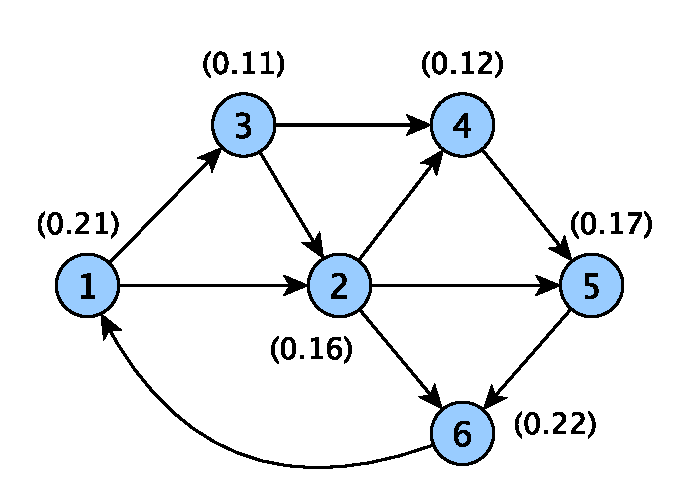
\includegraphics[width=0.5\textwidth]{figures/pagerank_example.pdf}
\caption{An example graph for PageRank}
\label{pagerank:example}
\end{figure}

PageRank is a link analysis algorithm that assigns a score to every vertex
measuring the relative importance of vertices within the set of all
vertices. PageRank~\cite{pagerank} was first used by Google to measure the
importance of website pages where the World Wide Web was modeled as a directed
graph. Figure~\ref{pagerank:example} shows an example graph with the PageRank
value of each vertex. The intuition behind the algorithm is that the number and
quality of links to a vertex determine the authoritativeness of the vertex,
which is reflected in the PageRank scores as shown in the figure.

The pagerank module in MADlib implements the model of a random surfer who
follows the edges of a graph to traverse it, and jumps to a random vertex
after several clicks. The random surfer is modeled using a damping factor
that represents the probability with which the surfer will continue to follow
links in the graph rather than jumping to a random vertex. MADlib's pagerank
module outputs a probability distribution that represents the likelihood that
the random surfer arrives at a particular vertex in the graph.

PageRank is an iterative algorithm where the PageRank scores of vertices from
the previous iteration are used to compute the new PageRank scores. The
PageRank score of a vertex $v$, at the $i^{th}$ iteration, denoted by $PR(v_i)$
is computed as:

\begin{equation}
PR(v_i) = \frac{1-d}{N} + d \sum_{u \in M(v)}(\frac{PR(u_{i-1})}{L(u)})
\label{eq:pagerank}
\end{equation}

where $N$ is the number of vertices in the graph, $d$ is the damping factor,
$M(v)$ represents the set of vertices that have an edge to vertex $v$,
$L(u)$ represents the out-degree of vertex $u$, i.e., the number of
out-going edges from vertex $u$, and $PR(u_{i-1})$ represents the PageRank
score of vertex $u$ in the $(i-1)^{st}$ iteration.

$\frac{1-d}{N}$ represents the tiny probability with which the surfer
would randomly jump to vertex $v$, rather than arriving at $v$ following
links in the graph. This ensures that there is some probability of visiting
every vertex in the graph even if they do not have any incoming edges. Note
that the PageRank score computed for a vertex $v$ using~\ref{eq:pagerank}
in the $i^{th}$ iteration is not updated until the new score is computed for
all the vertices in the graph. The computation terminates either when the
PageRank score of no vertex changes beyond a threshold across two consecutive
iterations, or when a pre-set number of iterations are completed.

\subsection{Implementation Details} \label{sec:pagerank:implementation}

In this section, we discuss the MADlib implementation of PageRank in depth.
We maintain two tables at every iteration: $previous$ and $cur$. The
$previous$ table maintains the PageRank scores of all vertices computed in
the previous iteration, while $cur$ maintains the updated scores of all
vertices in the current iteration.

\begin{algorithm}[PageRank$(V,E)$] \label{alg:pagerank:high}
\begin{algorithmic}[1]
    \State Create $previous$ table with a default PageRank score of
            $\frac{1}{N}$ for every vertex
    \Repeat
        \State Create empty table $cur$.
        \State Update $cur$ using PageRank scores of vertices in $previous$
        \State Update PageRank scores of vertices without incoming edges
        \State Drop $previous$ and rename $cur$ to $previous$
    \Until {PageRank scores have converged or \emph{max} iterations have elapsed}
\end{algorithmic}
\end{algorithm}

The implementation consists of updating the PageRank scores of all vertices
at every iteration, using the PageRank scores of vertices from the previous
iteration. The PageRank score of every vertex is initialized to $\frac{1}{N}$
where $N$ is the total number of vertices in the graph. The out-degree of
every vertex in the graph (represented by $L(u)$ in eq.~\ref{eq:pagerank}),
is captured in table $out\_cnts$. The following query is used to create and
update the PageRank scores in $cur$ table using the PageRank scores in
$previous$ table.

\begin{algorithm}[Update PageRank scores$(previous,out\_cnts,d,N)$]
\label{alg:pagerank:update}
\begin{lstlisting}
CREATE TABLE cur AS
    SELECT edge_table.dest AS id,
        SUM(previous1.pagerank/out_cnts.cnt)*d + (1-d)/N AS pagerank
    FROM edge_table
        INNER JOIN previous ON edge_table.dest = previous.id
        INNER JOIN out_cnts ON edge_table.src = out_cnts.id
        INNER JOIN previous AS previous1 ON edge_table.src = previous1.id
    GROUP BY edge_table.dest

-- Update PageRank scores of vertices without any incoming edges:
INSERT INTO cur
    SELECT id, (1-d)/N AS pagerank
    FROM previous
    WHERE id NOT IN (
        SELECT id
        FROM cur
    )
\end{lstlisting}
\end{algorithm}

The PageRank computation is terminated either when a fixed number of iterations
are completed, or when the PageRank scores of all vertices have converged. The
PageRank score of a vertex is deemed converged if the absolute difference in
its PageRank scores from $previous$ and $cur$ is less than a specified threshold.
The following query is used to find all the vertices whose PageRank scores have
not converged yet.

\begin{algorithm}[Update PageRank scores$(previous,cur,threshold)$]
\label{alg:pagerank:update}
\begin{lstlisting}
SELECT id
FROM cur
INNER JOIN previous ON cur.id = previous.id
WHERE ABS(previous.pagerank - cur.pagerank) > threshold
\end{lstlisting}
\end{algorithm}

\subsection{Best Practices} \label{sec:pagerank:bestpractices}

The pagerank module in MADlib has a few optional parameters: damping factor
$d$, number of iterations $max$, and the threshold for convergence $threshold$.
The default values for these parameters when not specified by the user are
$0.85$, $100$ and $\frac{1}{N*1000}$ respectively.

The damping factor denotes the probability with which the surfer uses the edges
to traverse the graph. If set to $0$, it implies that the only way a surfer
would visit a vertex in the graph is by randomly jumping to it. If set to
$1$, it implies that the only way the surfer can reach a vertex is by following
the edges in the graph, thus precluding the surfer from reaching a vertex
that has no incoming edges. It is common practice to set damping factor
to $0.85$~\cite{pagerank}, and the maximum number of iterations to $100$.
The convergence test for PageRank in MADlib checks for the delta between
the PageRank scores of a vertex across two consecutive iterations. Since
the initial value of the PageRank score is set to $\frac{1}{N}$, the delta
will be small in the initial iterations when $N$ is large (say over 100
million). We thus set the threshold to $\frac{1}{N*1000}$, and it is to be
noted that this is not based on any experimental study. Users of MADlib are
encouraged to consider this factor when setting a value for threshold, since
a high $threshold$ value would lead to early termination of PageRank
computation, thus resulting in incorrect PageRank values.


\section{Weakly Connected Components} \label{sec:graph:wcc}
\begin{figure}[h]
    \centering
    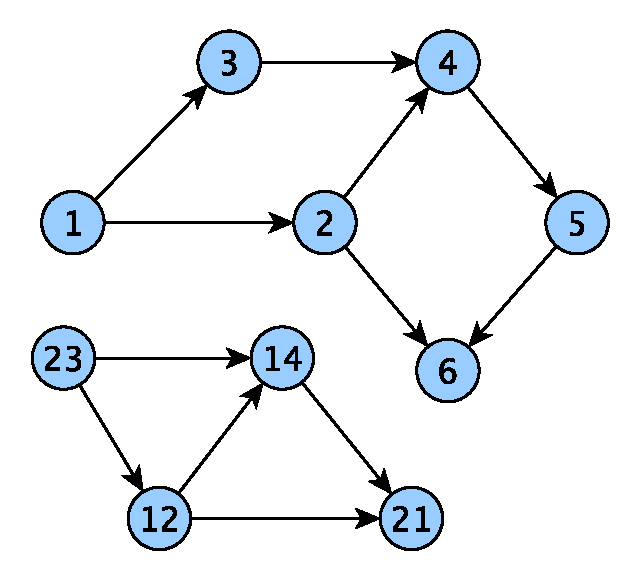
\includegraphics[width=0.5\textwidth]{figures/wcc_example.pdf}
\caption{An example disconnected directed graph}
\label{wcc:example}
\end{figure}

Given a directed graph $G$, a weakly connected component is a subgraph
$G_{sub}$ of $G$, such that there exists a path from every vertex in $G_{sub}$
to every other vertex in $G_{sub}$, ignoring the direction of the edges.

The weakly connected component module implemented in MADlib is based on
GRAIL~\cite{grail}. All vertices are initialized with their own vertex
ID as the component ID, and are considered to be active. In every iteration,
each active vertex's component ID is updated with the smallest component ID
value of all its neighbors. Any vertex whose component ID is not updated in
the current iteration is deemed as an inactive vertex for the next iteration.
Execution continues until there are no active vertices left. Since each vertex
is initialized with its own ID as the component ID, and updated based on
neighboring nodes' component IDs, the final component ID of a component will
be equal to the smallest vertex ID in the corresponding subgraph.
Figure~\ref{wcc:example} shows an example directed graph with two disconnected
subgraphs. The subgraph containing vertices $1$, $2$, $3$, $4$, $5$ and $6$
forms a weakly connected component, and is assigned component ID 1, while the
subgraph containing vertices $12$, $14$, $21$ and $23$ forms the second component
and is assigned component ID 12.

\subsection{Implementation Details} \label{sec:wcc:implementation}

In this section, we discuss the MADlib implementation of weakly connected
components in depth. We maintain the following tables at every iteration:
$oldupdate$, $message$ and $newupdate$. In $newupdate$, the component ID
of each vertex is initialized to infinity, while the component ID of vertices
in the $message$ table is initialized to their corresponding vertex ID.

\begin{algorithm}[Weakly Connected Components$(V,E)$] \label{alg:wcc:high}
\begin{algorithmic}[1]
    \State Create $newupdate$ table with a default component ID of
            $infinity$ for every vertex
    \State Create $message$ table with a default component ID of the
            corresponding $id$ (vertex ID) for every vertex
    \Repeat
        \State Update the $oldupdate$ table
        \State Update $toupdate$ table with active vertices
        \State Update the $newupdate$ table
        \State Update $message$ table with potential new component IDs for each vertex
    \Until {There are no active vertices in $toupdate$ table}
\end{algorithmic}
\end{algorithm}

The $message$ table contains the component IDs associated with all its
immediate neighbors. At each iteration, $oldupdate$ is updated with the
minimum of all the associated component IDs found for a vertex in $message$.

\begin{algorithm}[Update oldupdate table]
\begin{lstlisting}
SELECT id, MIN(message.component_id) as component_id
FROM message
GROUP BY id
\end{lstlisting}
\end{algorithm}

Table $toupdate$ records all vertices whose component IDs must be updated,
and are thus marked active.

\begin{algorithm}[Update toupdate table with active vertices]
\begin{lstlisting}
-- Find vertices whose component ID must be updated
CREATE TABLE toupdate AS
SELECT id, component_id
FROM oldupdate, newupdate
WHERE oldupdate.id = newupdate.id AND
        oldupdate.component_id < newupdate.component_id

-- Update the component IDs
UPDATE newupdate SET
component_id = toupdate.component_id
FROM toupdate
WHERE newupdate.id = toupdate.id
\end{lstlisting}
\end{algorithm}

Finally, the $message$ table is updated with potential new
component IDs for active vertices using the following query:

\begin{algorithm}[Update oldupdate table]
\begin{lstlisting}
CREATE TEMP TABLE message AS
SELECT id, MIN(component_id) AS component_id
FROM (
    SELECT edge.src AS id,
        toupdate.component_id
    FROM toupdate, edge
    WHERE edge.dest = toupdate.id
    UNION ALL
    SELECT edge.dest AS id,
        toupdate.component_id
    FROM toupdate, edge
    WHERE edge.src = toupdate.id
) AS t
GROUP BY id
\end{lstlisting}
\end{algorithm}

At the end of the computation, $newupdate$ will have the component ID
associated with each vertex in $G$. The component ID of all the vertices
in a component is equal to the smallest vertex ID in the corresponding
subgraph.

\section{Breadth-first Search} \label{sec:graph:bfs}

Given a graph $G$ and a user-specified origin vertex $src$, this algorithm
searches and discovers connected nodes in a graph in breadth-first order
\cite{bfs_wikipedia}. The graph can be treated as either directed or
undirected based on a parameter specified when calling the function.
There is also a parameter to control the number of hops (edges) to traverse
from the source vertex. If not specified, all nodes accessible from the
source node will be discovered.

\subsection{Implementation Details}
\begin{algorithm}[Breadth First Search$(V, E, src)$] \label{alg:bfs:high}
\begin{algorithmic}[1]
    \State Set $dist \leftarrow 0$
    \State Create $message$ table with $src$ vertex, $NULL$ parent, and $dist$
    \State Copy $message$ table to output table $out$
    \Repeat
        \State Create $toupdate$ table using $out$ and $message$ tables
        \State $dist \leftarrow dist + 1$
        \State Update $message$ table with newly found candidate vertices, parent and $dist$
        \State Copy $message$ table to $out$
    \Until {There are no candidate vertices remaining in $message$ table}
\end{algorithmic}
\end{algorithm}

The implementation details are similar to SSSP, albeit simpler. We only have to
track the number of hops and not the sum of weights, but other requirements and
restrictions such as finding the parent, distinct updates, etc. are common in
both cases. The output table is initialized only to the $src$ vertex to begin
with. A $message$ table is also maintained that contains the list of vertices
to traverse and explore in the next iteration, which is also initialized with
the $src$ vertex. BFS then runs iteratively until no more candidate vertices
remain in the $message$ table, as outlined in~\ref{alg:bfs:high}.

At every iteration, $toupdate$ table is updated with vertices that are neighbors
of vertices in the $message$ table, that are not already visited in the past
(one scan of the $out$ table reveals all the vertices that have already been
visited in the past). All such newly found neighboring vertices in the current
iteration will have one or more parents, based on how many vertices in the
$message$ table have a direct edge to them. Each such vertex in the $message$
table is marked as the parent of such newly found neighboring vertices in
the $toupdate$ table.

The $message$ table is then cleared and updated with the contents of $toupdate$
table, except that for each new neighboring vertex considered, only one of the
parents is recorded as its parent (the node with the smallest id among all
parent nodes). The content of this updated $message$ is then copied
to the $out$ table, and this process continues until $message$ table is empty.

% Licensed to the Apache Software Foundation (ASF) under one
% or more contributor license agreements.  See the NOTICE file
% distributed with this work for additional information
% regarding copyright ownership.  The ASF licenses this file
% to you under the Apache License, Version 2.0 (the
% "License"); you may not use this file except in compliance
% with the License.  You may obtain a copy of the License at

%   http://www.apache.org/licenses/LICENSE-2.0

% Unless required by applicable law or agreed to in writing,
% software distributed under the License is distributed on an
% "AS IS" BASIS, WITHOUT WARRANTIES OR CONDITIONS OF ANY
% KIND, either express or implied.  See the License for the
% specific language governing permissions and limitations
% under the License.

% When using TeXShop on the Mac, let it know the root document.
% The following must be one of the first 20 lines.
% !TEX root = ../design.tex

\chapter{Neural Network}

\begin{moduleinfo}
\item[Authors] {Xixuan Feng}
\end{moduleinfo}

% Abstract. What is the problem we want to solve?
This module implements artificial neural network \cite{ann_wiki}.

\section{Multilayer Perceptron}
Multilayer perceptron is arguably the most popular model among many neural network models \cite{mlp_wiki}.
Here, we learn the coefficients by minimizing a least square objective function (\cite{bertsekas1999nonlinear}, example 1.5.3).

% Background. Why can we solve the problem with gradient-based methods?
\subsection{Solving as a Convex Program}
Although the objective function is not necessarily convex, gradient descent or incremental gradient descent are still commonly-used algorithms to learn the coefficients.
To clarify, gradient-based methods are not different from the famous backpropagation, which is essentially a way to compute the gradient value.

\subsection{Formal Description}
Having the convex programming framework, the main tasks of implementing a learner include:
(a) choose a subset of algorithms;
(b) implement the related computation logic for the objective function, e.g., gradient.

For multilayer perceptron, we choose incremental gradient descent (IGD).
In the remaining part of this section, we will give a formal description of the derivation of objective function and its gradient.

\paragraph{Objective function.}
We mostly follow the notations in example 1.5.3 from Bertsekas \cite{bertsekas1999nonlinear}, for a multilayer perceptron that has $N$ layers (stages), and the $k$th stage has $n_k$ activation units ($\phi : \mathbb{R} \to \mathbb{R}$), the objective function is given as
\[f_{(y, z)}(u) = \frac{1}{2} \|h(u, y) - z\|_2^2,\]
where $y \in \mathbb{R}^{n_0}$ is the input vector, $z \in \mathbb{R}^{n_N}$ is the output vector,
\footnote{Of course, the objective function can be defined over a set of input-output vector pairs, which is simply given as the addition of the above $f$.}
and the coefficients are given as
\[u = \{ u_{k-1}^{sj} \; | \; k = 1,...,N, \: s = 0,...,n_{k-1}, \: j = 1,...,n_k\}\]
This still leaves $h : \mathbb{R}^{n_0} \to \mathbb{R}^{n_N}$ as an open item.
Let $x_k \in \mathbb{R}^{n_k}, k = 1,...,N$ be the output vector of the $k$th layer. Then we define $h(u, y) = x_N$, based on setting $x_0 = y$ and the $j$th component of $x_k$ is given in an iterative fashion as
\footnote{$x_k^0 \equiv 1$ is used to simplified the notations, and $x_k^0$ is not a component of $x_k$, for any $k = 0,...,N$.}
\[\begin{alignedat}{5}
    x_k^j = \phi \left( \sum_{s=0}^{n_{k-1}} x_{k-1}^s u_{k-1}^{sj} \right), &\quad k = 1,...,N, \; j = 1,...,n_k
\end{alignedat}\]

\paragraph{Gradient of the End Layer.}
Let's first handle $u_{N-1}^{st}, s = 0,...,n_{N-1}, t = 1,...,n_N$.
Let $z^t$ denote the $t$th component of $z \in \mathbb{R}^{n_N}$, and $h^t$ the $t$th component of output of $h$.
\[\begin{aligned}
    \frac{\partial f}{\partial u_{N-1}^{st}}
    &= \left( h^t(u, y) - z^t \right) \cdot \frac{\partial h^t(u, y)}{\partial u_{N-1}^{st}} \\
    &= \left( x_N^t - z^t \right) \cdot \frac{\partial x_N^t}{\partial u_{N-1}^{st}} \\
    &= \left( x_N^t - z^t \right) \cdot \frac{\partial \phi \left( \sum_{s=0}^{n_{N-1}} x_{N-1}^s u_{N-1}^{st} \right)}{\partial u_{N-1}^{st}} \\
    &= \left( x_N^t - z^t \right) \cdot \phi' \left( \sum_{s=0}^{n_{N-1}} x_{N-1}^s u_{N-1}^{st} \right) \cdot x_{N-1}^s \\
\end{aligned}\]
To ease the notation, let the input vector of the $j$th activation unit of the $(k+1)$th layer be
\[\mathit{net}_k^j =\sum_{s=0}^{n_{k-1}} x_{k-1}^s u_{k-1}^{sj},\]
where $k = 1,...,N, \; j = 1,...,n_k$, and note that $x_k^j =\phi(\mathit{net}_k^j)$. Finally, the gradient
\[\frac{\partial f}{\partial u_{N-1}^{st}} = \left( x_N^t - z^t \right) \cdot \phi' ( \mathit{net}_N^t ) \cdot x_{N-1}^s\]
For any $s = 0,...,n_{N-1}, t =1,...,n_N$, we are given $z^t$, and $x_N^t, \mathit{net}_N^t, x_{N-1}^s$ can be computed by forward iterating the network layer by layer (also called the feed-forward pass). Therefore, we now know how to compute the coefficients for the end layer $u_{N-1}^{st}, s = 0,...,n_{N-1}, t =1,...,n_N$.

\subsubsection{Backpropagation}
For inner (hidden) layers, it is more difficult to compute the partial derivative over the input of activation units (i.e., $\mathit{net}_k, k = 1,...,N-1$).
That said, $\frac{\partial f}{\partial \mathit{net}_N^t} = (x_N^t - z^t) \phi'(\mathit{net}_N^t)$ is easy, where $t = 1,...,n_N$, but $\frac{\partial f}{\partial \mathit{net}_k^j}$ is hard, where $k = 1,...,N-1, j = 1,..,n_k$.
This hard-to-compute statistic is referred to as \textit{delta error}, and let $\delta_k^j = \frac{\partial f}{\partial \mathit{net}_k^j}$, where $k = 1,...,N-1, j = 1,..,n_k$.
If this is solved, the gradient can be easily computed as follow
\[\frac{\partial f}{\partial u_{k-1}^{sj}} = \boxed{\frac{\partial f}{\partial \mathit{net}_k^j}} \cdot \frac{\partial \mathit{net}_k^j}{\partial u_{k-1}^{sj}} = \boxed{\delta_k^j} x_{k-1}^s,\]
where $k = 1,...,N-1, s = 0,...,n_{k-1}, j = 1,..,n_k$.
To solve this, we introduce the popular backpropagation below.

\paragraph{Error Back Propagation.}
Since we know how to compute $\delta_N^t, t = 1,...,n_N$, we try to compute $\delta_{k}^j, j = 1,...,n_{k}$, given $\delta_{k+1}^t, t = 1,...,n_{k+1}$, for any $k = 1,...,N-1$.
First,
\[
    \delta_{k}^j
    = \frac{\partial f}{\partial \mathit{net}_{k}^j}
    = \frac{\partial f}{\partial x_{k}^j} \cdot \frac{\partial x_{k}^j}{\partial \mathit{net}_{k}^j}
    = \frac{\partial f}{\partial x_{k}^j} \cdot \phi'(\mathit{net}_{k}^j)
\]
And here comes the only equation that is needed but the author, I (Aaron), do not understand but it looks reasonable and repeats in different online notes \cite{mlp_gradient_wisc},
\[\begin{alignedat}{5}
    \frac{\partial f}{\partial x_{k}^j} = \sum_{t=1}^{n_{k+1}} \left( \frac{\partial f}{\partial \mathit{net}_{k+1}^t} \cdot \frac{\partial \mathit{net}_{k+1}^t}{\partial x_{k}^j} \right),
    &\quad k = 1,...,N-1, \: j = 1,...,n_{k}
\end{alignedat}\]
Assuming the above equation is true, we can solve delta error backward iteratively
\[\begin{aligned}
    \delta_{k}^j
    &= \frac{\partial f}{\partial x_{k}^j} \cdot \phi'(\mathit{net}_{k}^j) \\
    &= \sum_{t=1}^{n_{k+1}} \left( \frac{\partial f}{\partial \mathit{net}_{k+1}^t} \cdot \frac{\partial \mathit{net}_{k+1}^t}{\partial x_{k}^j} \right) \cdot \phi'(\mathit{net}_{k}^j) \\
    &= \sum_{t=1}^{n_{k+1}} \left( \delta_{k+1}^t \cdot \frac{\partial \left( \sum_{s=0}^{n_{k}} x_{k}^s u_{k}^{st} \right) }{\partial x_{k}^j} \right) \cdot \phi'(\mathit{net}_{k}^j) \\
    &= \sum_{t=1}^{n_{k+1}} \left( \delta_{k+1}^t \cdot u_{k}^{jt} \right) \cdot \phi'(\mathit{net}_{k}^j) \\
\end{aligned}\]
To sum up, we need the following equation for error back propagation
\[\boxed{\delta_{k}^j = \sum_{t=1}^{n_{k+1}} \left( \delta_{k+1}^t \cdot u_{k}^{jt} \right) \cdot \phi'(\mathit{net}_{k}^j)}\]
where $k = 1,...,N-1$, and $j = 1,...,n_{k}$.

\subsubsection{The $\mathit{Gradient}$ Function}
\begin{algorithm}[mlp-gradient$(u, y, z)$] \label{alg:mlp-gradient}
\alginput{Coefficients $u = \{ u_{k-1}^{sj} \; | \; k = 1,...,N, \: s = 0,...,n_{k-1}, \: j = 1,...,n_k\}$,\\
start vector $y \in \mathbb{R}^{n_0}$,\\
end vector $z \in \mathbb{R}^{n_N}$,\\
activation unit $\phi : \mathbb{R} \to \mathbb{R}$}
\algoutput{Gradient value $\nabla f(u)$ that consists of components $\nabla f(u)_{k-1}^{sj} = \frac{\partial f}{\partial u_{k-1}^{sj}}$}
\begin{algorithmic}[1]
    \State $(\mathit{net}, x) \set$ \texttt{feed-forward}$(u, y, \phi)$
    \State $\delta_N \set$ \texttt{end-layer-delta-error}$(\mathit{net}, x, z, \phi')$
    \State $\delta \set$ \texttt{error-back-propagation}$(\delta_N, \mathit{net}, u, \phi')$
    \For{$k = 1,...,N$}
        \For{$s = 0,...,n_{k-1}$}
            \For{$j = 1,...,n_k$}
                \State $\nabla f(u)_{k-1}^{sj} \set \delta_k^j x_{k-1}^s$
                \Comment{Can be put together with the computation of delta $\delta$}
            \EndFor
        \EndFor
    \EndFor
    \State \Return $\nabla f(u)$
\end{algorithmic}
\end{algorithm}

\paragraph{Activation Units $\phi$.}
Common examples of activation units are
\[\begin{alignedat}{3}
\phi(\xi) &= \frac{1}{1 + e^{-\xi}}, &\quad \text{ (logistic function),}\\
\phi(\xi) &= \frac{e^{\xi} - e^{-\xi}}{e^{\xi} + e^{-\xi}}, &\quad \text{ (hyperbolic tangent function)}\\
\end{alignedat}\]

\begin{algorithm}[feed-forward$(u, y, \phi)$] \label{alg:feed-forward}
\alginput{Coefficients $u = \{ u_{k-1}^{sj} \; | \; k = 1,...,N, \: s = 0,...,n_{k-1}, \: j = 1,...,n_k\}$,\\
input vector $y \in \mathbb{R}^{n_0}$,\\
activation unit $\phi : \mathbb{R} \to \mathbb{R}$}
\algoutput{Input vectors $\mathit{net} = \{\mathit{net}_k^j \; | \; k = 1,...,N, \: j = 1,...,n_k\}$,\\
output vectors $x = \{x_k^j \; | \; k = 0,...,N, \: j = 0,...,n_k\}$}
\begin{algorithmic}[1]
    \For{$k = 0,...,N$}
        \State $x_k^0 \set 1$
    \EndFor
    \State $x_0 \set y$ \Comment{For all components $x_0^j, y^j, \; j = 1,...,n_0$}
    \For{$k = 1,...,N$}
        \For{$j = 1,...,n_k$}
            \State $\mathit{net}_k^j \set 0$
            \For{$s = 0,...,n_{k-1}$}
                \State $\mathit{net}_k^j \set \mathit{net}_k^j + x_{k-1}^s u_{k-1}^{sj}$
            \EndFor
            \State $x_k^j = \phi(\mathit{net}_k^j)$
        \EndFor
    \EndFor
    \State \Return $(\mathit{net}, x)$
\end{algorithmic}
\end{algorithm}

\begin{algorithm}[end-layer-delta-error$(\mathit{net}, x, z, \phi')$] \label{alg:end-layer-delta-error}
\alginput{Input vectors $\mathit{net} = \{\mathit{net}_k^j \; | \; k = 1,...,N, \: j = 1,...,n_k\}$,\\
output vectors $x = \{x_k^j \; | \; k = 0,...,N, \: j = 0,...,n_k\}$,\\
end vector $z \in \mathbb{R}^{n_N}$,\\
derivative of activation unit $\phi' : \mathbb{R} \to \mathbb{R}$}
\algoutput{End layer delta $\delta_N = \{\delta_N^t \; | \; t = 1,...,n_N\}$}
\begin{algorithmic}[1]
    \For{$t = 1,...,n_N$}
            \State $\delta_N^t \set (x_N^t - z^t) \phi'(\mathit{net}_N^t)$
    \EndFor
    \State \Return $\delta_N$
\end{algorithmic}
\end{algorithm}

\begin{algorithm}[error-back-propagation$(\delta_N, \mathit{net}, u, \phi')$] \label{alg:error-back-propagation}
\alginput{End layer delta $\delta_N = \{\delta_N^t \; | \; t = 1,...,n_N\}$,\\
input vectors $\mathit{net} = \{\mathit{net}_k^j \; | \; k = 1,...,N, \: j = 1,...,n_k\}$,\\
coefficients $u = \{ u_{k-1}^{sj} \; | \; k = 1,...,N, \: s = 0,...,n_{k-1}, \: j = 1,...,n_k\}$,\\
derivative of activation unit $\phi' : \mathbb{R} \to \mathbb{R}$}
\algoutput{Delta $\delta = \{\delta_k^j \; | \; k = 1,...,N, \: j = 1,...,n_k\}$}
\begin{algorithmic}[1]
    \For{$k = N-1,...,1$}
        \For{$j = 0,...,n_k$}
            \State $\delta_k^j \set 0$
            \For{$t = 1,...,n_{k+1}$}
                \State $\delta_k^j \set \delta_k^j + \delta_{k+1}^t u_k^{jt}$
            \EndFor
            \State $\delta_k^j \set \delta_k^j \phi'(\mathit{net}_k^j)$
        \EndFor
    \EndFor
    \State \Return $\delta$
\end{algorithmic}
\end{algorithm}

\printbibliography

\end{document}
